% Options for packages loaded elsewhere
% Options for packages loaded elsewhere
\PassOptionsToPackage{unicode}{hyperref}
\PassOptionsToPackage{hyphens}{url}
\PassOptionsToPackage{dvipsnames,svgnames,x11names}{xcolor}
%
\documentclass[
  a4paper,
]{book}
\usepackage{xcolor}
\usepackage[top=2.5cm,bottom=2.5cm,left=2.5cm,right=2.5cm]{geometry}
\usepackage{amsmath,amssymb}
\setcounter{secnumdepth}{5}
\usepackage{iftex}
\ifPDFTeX
  \usepackage[T1]{fontenc}
  \usepackage[utf8]{inputenc}
  \usepackage{textcomp} % provide euro and other symbols
\else % if luatex or xetex
  \usepackage{unicode-math} % this also loads fontspec
  \defaultfontfeatures{Scale=MatchLowercase}
  \defaultfontfeatures[\rmfamily]{Ligatures=TeX,Scale=1}
\fi
\usepackage{lmodern}
\ifPDFTeX\else
  % xetex/luatex font selection
\fi
% Use upquote if available, for straight quotes in verbatim environments
\IfFileExists{upquote.sty}{\usepackage{upquote}}{}
\IfFileExists{microtype.sty}{% use microtype if available
  \usepackage[]{microtype}
  \UseMicrotypeSet[protrusion]{basicmath} % disable protrusion for tt fonts
}{}
\makeatletter
\@ifundefined{KOMAClassName}{% if non-KOMA class
  \IfFileExists{parskip.sty}{%
    \usepackage{parskip}
  }{% else
    \setlength{\parindent}{0pt}
    \setlength{\parskip}{6pt plus 2pt minus 1pt}}
}{% if KOMA class
  \KOMAoptions{parskip=half}}
\makeatother
% Make \paragraph and \subparagraph free-standing
\makeatletter
\ifx\paragraph\undefined\else
  \let\oldparagraph\paragraph
  \renewcommand{\paragraph}{
    \@ifstar
      \xxxParagraphStar
      \xxxParagraphNoStar
  }
  \newcommand{\xxxParagraphStar}[1]{\oldparagraph*{#1}\mbox{}}
  \newcommand{\xxxParagraphNoStar}[1]{\oldparagraph{#1}\mbox{}}
\fi
\ifx\subparagraph\undefined\else
  \let\oldsubparagraph\subparagraph
  \renewcommand{\subparagraph}{
    \@ifstar
      \xxxSubParagraphStar
      \xxxSubParagraphNoStar
  }
  \newcommand{\xxxSubParagraphStar}[1]{\oldsubparagraph*{#1}\mbox{}}
  \newcommand{\xxxSubParagraphNoStar}[1]{\oldsubparagraph{#1}\mbox{}}
\fi
\makeatother


\usepackage{longtable,booktabs,array}
\newcounter{none} % for unnumbered tables
\usepackage{calc} % for calculating minipage widths
% Correct order of tables after \paragraph or \subparagraph
\usepackage{etoolbox}
\makeatletter
\patchcmd\longtable{\par}{\if@noskipsec\mbox{}\fi\par}{}{}
\makeatother
% Allow footnotes in longtable head/foot
\IfFileExists{footnotehyper.sty}{\usepackage{footnotehyper}}{\usepackage{footnote}}
\makesavenoteenv{longtable}
\usepackage{graphicx}
\makeatletter
\newsavebox\pandoc@box
\newcommand*\pandocbounded[1]{% scales image to fit in text height/width
  \sbox\pandoc@box{#1}%
  \Gscale@div\@tempa{\textheight}{\dimexpr\ht\pandoc@box+\dp\pandoc@box\relax}%
  \Gscale@div\@tempb{\linewidth}{\wd\pandoc@box}%
  \ifdim\@tempb\p@<\@tempa\p@\let\@tempa\@tempb\fi% select the smaller of both
  \ifdim\@tempa\p@<\p@\scalebox{\@tempa}{\usebox\pandoc@box}%
  \else\usebox{\pandoc@box}%
  \fi%
}
% Set default figure placement to htbp
\def\fps@figure{htbp}
\makeatother


% definitions for citeproc citations
\NewDocumentCommand\citeproctext{}{}
\NewDocumentCommand\citeproc{mm}{%
  \begingroup\def\citeproctext{#2}\cite{#1}\endgroup}
\makeatletter
 % allow citations to break across lines
 \let\@cite@ofmt\@firstofone
 % avoid brackets around text for \cite:
 \def\@biblabel#1{}
 \def\@cite#1#2{{#1\if@tempswa , #2\fi}}
\makeatother
\newlength{\cslhangindent}
\setlength{\cslhangindent}{1.5em}
\newlength{\csllabelwidth}
\setlength{\csllabelwidth}{3em}
\newenvironment{CSLReferences}[2] % #1 hanging-indent, #2 entry-spacing
 {\begin{list}{}{%
  \setlength{\itemindent}{0pt}
  \setlength{\leftmargin}{0pt}
  \setlength{\parsep}{0pt}
  % turn on hanging indent if param 1 is 1
  \ifodd #1
   \setlength{\leftmargin}{\cslhangindent}
   \setlength{\itemindent}{-1\cslhangindent}
  \fi
  % set entry spacing
  \setlength{\itemsep}{#2\baselineskip}}}
 {\end{list}}
\usepackage{calc}
\newcommand{\CSLBlock}[1]{\hfill\break\parbox[t]{\linewidth}{\strut\ignorespaces#1\strut}}
\newcommand{\CSLLeftMargin}[1]{\parbox[t]{\csllabelwidth}{\strut#1\strut}}
\newcommand{\CSLRightInline}[1]{\parbox[t]{\linewidth - \csllabelwidth}{\strut#1\strut}}
\newcommand{\CSLIndent}[1]{\hspace{\cslhangindent}#1}



\setlength{\emergencystretch}{3em} % prevent overfull lines

\providecommand{\tightlist}{%
  \setlength{\itemsep}{0pt}\setlength{\parskip}{0pt}}



 


\usepackage{xcolor}
\usepackage{centernot}
\definecolor{isublue}{RGB}{30,56,100}
\definecolor{accent}{RGB}{46,117,182}
\definecolor{darkgrey}{RGB}{80,80,80}
\renewcommand{\maketitle}{}
\newcommand{\doop}{\operatorname{do}}
\newcommand{\indep}{\perp\!\!\!\perp}
\newcommand{\nindep}{\centernot{\indep}}
\newcommand{\E}{\mathbb{E}}
\newcommand{\Gcal}{\mathcal{G}}
\newcommand{\Pa}{\mathrm{Pa}}
\newcommand{\De}{\mathrm{De}}
\newcommand{\An}{\mathrm{An}}
\newcommand{\Nd}{\mathrm{Nd}}
\newcommand{\pto}{\overset{p}{\to}}
\newcommand{\expit}{\operatorname{expit}}
\AtBeginDocument{%
  \begin{titlepage}
    \centering
    \vspace*{3cm}
    {\Huge\bfseries\color{isublue}
      Theory and Methods in Causal Inference}\\[1.2cm]
    {\LARGE\color{accent} Lecture Notes}\\[0.8cm]
    \color{accent}\rule{0.6\textwidth}{1.2pt}\\[0.8cm]
    {\large Jae Kwang Kim \\[0.3cm]
      Department of Statistics\\[0.3cm]
      Iowa State University}\\[2cm]
    {\normalsize STAT 5900B}\\[0.8cm]
    {\normalsize\color{darkgrey} Last updated: \today}\\[0.3cm]
    \vfill
  \end{titlepage}
  \tableofcontents
  \newpage
}
\makeatletter
\@ifpackageloaded{tcolorbox}{}{\usepackage[skins,breakable]{tcolorbox}}
\@ifpackageloaded{fontawesome5}{}{\usepackage{fontawesome5}}
\definecolor{quarto-callout-color}{HTML}{909090}
\definecolor{quarto-callout-note-color}{HTML}{0758E5}
\definecolor{quarto-callout-important-color}{HTML}{CC1914}
\definecolor{quarto-callout-warning-color}{HTML}{EB9113}
\definecolor{quarto-callout-tip-color}{HTML}{00A047}
\definecolor{quarto-callout-caution-color}{HTML}{FC5300}
\definecolor{quarto-callout-color-frame}{HTML}{acacac}
\definecolor{quarto-callout-note-color-frame}{HTML}{4582ec}
\definecolor{quarto-callout-important-color-frame}{HTML}{d9534f}
\definecolor{quarto-callout-warning-color-frame}{HTML}{f0ad4e}
\definecolor{quarto-callout-tip-color-frame}{HTML}{02b875}
\definecolor{quarto-callout-caution-color-frame}{HTML}{fd7e14}
\makeatother
\makeatletter
\@ifpackageloaded{bookmark}{}{\usepackage{bookmark}}
\makeatother
\makeatletter
\@ifpackageloaded{caption}{}{\usepackage{caption}}
\AtBeginDocument{%
\ifdefined\contentsname
  \renewcommand*\contentsname{Table of contents}
\else
  \newcommand\contentsname{Table of contents}
\fi
\ifdefined\listfigurename
  \renewcommand*\listfigurename{List of Figures}
\else
  \newcommand\listfigurename{List of Figures}
\fi
\ifdefined\listtablename
  \renewcommand*\listtablename{List of Tables}
\else
  \newcommand\listtablename{List of Tables}
\fi
\ifdefined\figurename
  \renewcommand*\figurename{Figure}
\else
  \newcommand\figurename{Figure}
\fi
\ifdefined\tablename
  \renewcommand*\tablename{Table}
\else
  \newcommand\tablename{Table}
\fi
}
\@ifpackageloaded{float}{}{\usepackage{float}}
\floatstyle{ruled}
\@ifundefined{c@chapter}{\newfloat{codelisting}{h}{lop}}{\newfloat{codelisting}{h}{lop}[chapter]}
\floatname{codelisting}{Listing}
\newcommand*\listoflistings{\listof{codelisting}{List of Listings}}
\makeatother
\makeatletter
\makeatother
\makeatletter
\@ifpackageloaded{caption}{}{\usepackage{caption}}
\@ifpackageloaded{subcaption}{}{\usepackage{subcaption}}
\makeatother
\usepackage{bookmark}
\IfFileExists{xurl.sty}{\usepackage{xurl}}{} % add URL line breaks if available
\urlstyle{same}
\hypersetup{
  pdftitle={Theory and Methods in Causal Inference},
  pdfauthor={Jae-kwang Kim},
  colorlinks=true,
  linkcolor={Maroon},
  filecolor={Maroon},
  citecolor={Blue},
  urlcolor={Blue},
  pdfcreator={LaTeX via pandoc}}


\title{Theory and Methods in Causal Inference}
\author{Jae-kwang Kim}
\date{2026-04-14}
\begin{document}
\frontmatter
\maketitle


\mainmatter
\bookmarksetup{startatroot}

\chapter*{Preface}\label{preface}
\addcontentsline{toc}{chapter}{Preface}

\markboth{Preface}{Preface}

These lecture notes accompany the graduate course \textbf{STAT 5900B:
Theory and Methods in Causal Inference} at the Department of Statistics,
Iowa State University.

The course targets graduate students in statistics. It assumes
familiarity with probability theory, mathematical statistics, and linear
models at the level of a graduate sequence, but no prior exposure to
causal inference.

📄 \href{Theory-and-Methods-in-Causal-Inference.pdf}{Download full PDF}

\section*{Organization}\label{organization}
\addcontentsline{toc}{section}{Organization}

\markright{Organization}

The notes are organized in four parts.

\textbf{Part I --- Foundations} (Chapters 1--4) builds the graphical and
conceptual foundation: the causal trinity (SEM, DAG, potential
outcomes), DAGs and d-separation, the do-calculus and identification
criteria, and the connection between potential outcomes and the
do-calculus.

\textbf{Part II --- Identification} (Chapters 5--8) bridges the
graphical framework and observed data: randomization and back-door
adjustment, propensity score methods, instrumental variables, and
mediation and front-door identification.

\textbf{Part III --- Estimation} (Chapters 9--12) covers semiparametric
efficiency theory: estimating equations and influence functions, doubly
robust estimation, flexible nuisance estimation with cross-fitting, and
estimation under instrumental variables.

\textbf{Part IV --- Policy Learning and Sequential Decision Making}
(Chapters 13--15) covers policy evaluation, optimal policy learning, and
dynamic treatment regimes.

\section*{Notation}\label{notation}
\addcontentsline{toc}{section}{Notation}

\markright{Notation}

Throughout these notes:

\begin{itemize}
\tightlist
\item
  \(\doop(T = t)\) denotes the do-operator (intervention).
\item
  \(Y(t)\) denotes the potential outcome under \(T = t\).
\item
  \(\E[\,\cdot\,]\) denotes expectation; \(\indep\) denotes conditional
  independence.
\item
  \(\mathcal{G}\) denotes a DAG; \(\mathcal{G}_T\) denotes the mutilated
  graph after intervening on \(T\).
\end{itemize}

\bookmarksetup{startatroot}

\chapter{Introduction}\label{introduction}

\begin{tcolorbox}[enhanced jigsaw, arc=.35mm, bottomrule=.15mm, bottomtitle=1mm, breakable, colback=white, colbacktitle=quarto-callout-note-color!10!white, colframe=quarto-callout-note-color-frame, coltitle=black, left=2mm, leftrule=.75mm, opacityback=0, opacitybacktitle=0.6, rightrule=.15mm, title={Learning Objectives}, titlerule=0mm, toprule=.15mm, toptitle=1mm]

By the end of this chapter, students should be able to:

\begin{enumerate}
\def\labelenumi{\arabic{enumi}.}
\tightlist
\item
  Articulate the distinction between an interventional distribution
  \(f(y \mid \doop(T{=}t))\) and an observational conditional
  distribution \(f(y \mid T{=}t)\), and explain why they differ whenever
  \(T\) is endogenous.
\item
  Describe the same causal question in all three languages --- SEM, DAG
  graph surgery, and potential outcomes --- and begin to translate
  between them.
\item
  Derive the two densities explicitly in the Gaussian linear confounded
  model, and identify the endogeneity bias
  \(\alpha\gamma\sigma_U^2/\sigma_T^2\) as the gap between them.
\item
  State the two-step paradigm (identification then estimation) and
  locate each step in the causal inference pipeline.
\end{enumerate}

\end{tcolorbox}

This chapter is an orientation, not a complete treatment. It introduces
four ideas --- the interventional/observational distinction, the causal
trinity, the Gaussian confounded model as a running example, and the
identification-versus-estimation paradigm --- that will be developed
rigorously in Chapters 2--4 and beyond.

\section{Motivation: Why Causal Inference Is
Hard}\label{motivation-why-causal-inference-is-hard}

Causal inference studies when and how the observational distribution can
be used to recover the distribution that would arise under
interventions.

\subsection{The Central Question}\label{the-central-question}

Causal inference is concerned with a deceptively simple question: what
would happen to \(Y\) if we were to \emph{set} \(T = t\)? This is
fundamentally different from the question that standard statistical
procedures answer: what is the distribution of \(Y\) among units
\emph{observed} to have \(T = t\)?

\begin{tcolorbox}[enhanced jigsaw, arc=.35mm, bottomrule=.15mm, bottomtitle=1mm, breakable, colback=white, colbacktitle=quarto-callout-note-color!10!white, colframe=quarto-callout-note-color-frame, coltitle=black, left=2mm, leftrule=.75mm, opacityback=0, opacitybacktitle=0.6, rightrule=.15mm, title={Definition: Interventional vs.~Observational Distribution}, titlerule=0mm, toprule=.15mm, toptitle=1mm]

\begin{itemize}
\tightlist
\item
  The \emph{interventional distribution} \(f(y \mid \doop(T{=}t))\) is
  the distribution of \(Y\) in a hypothetical world where \(T\) has been
  \emph{externally set} to \(t\), regardless of the usual
  data-generating mechanism for \(T\).
\item
  The \emph{observational conditional distribution} \(f(y \mid T{=}t)\)
  is the distribution of \(Y\) among the subpopulation of units for whom
  \(T = t\) was \emph{observed} to hold.
\end{itemize}

These two distributions coincide only when \(T\) is randomized
(exogenous). In all other cases they differ, and the difference is
\emph{endogeneity bias}.

\end{tcolorbox}

\begin{tcolorbox}[enhanced jigsaw, arc=.35mm, bottomrule=.15mm, bottomtitle=1mm, breakable, colback=white, colbacktitle=quarto-callout-note-color!10!white, colframe=quarto-callout-note-color-frame, coltitle=black, left=2mm, leftrule=.75mm, opacityback=0, opacitybacktitle=0.6, rightrule=.15mm, title={Definition: Exogeneity and Endogeneity}, titlerule=0mm, toprule=.15mm, toptitle=1mm]

Suppose the outcome is generated by the structural equation
\(Y = f_Y(T, X, U)\), where \(T\) is the treatment, \(X\) are observed
covariates, and \(U\) represents unobserved common causes of \(T\) and
\(Y\) (confounders).

\begin{itemize}
\tightlist
\item
  The treatment \(T\) is \emph{exogenous given \(X\)} if
  \(T \indep U \mid X\).
\item
  The treatment \(T\) is \emph{endogenous given \(X\)} if
  \(T \nindep U \mid X\), so that some unobserved variable \(U\) affects
  both \(T\) and \(Y\).
\end{itemize}

\end{tcolorbox}

\begin{tcolorbox}[enhanced jigsaw, arc=.35mm, bottomrule=.15mm, bottomtitle=1mm, breakable, colback=white, colbacktitle=quarto-callout-note-color!10!white, colframe=quarto-callout-note-color-frame, coltitle=black, left=2mm, leftrule=.75mm, opacityback=0, opacitybacktitle=0.6, rightrule=.15mm, title={Example: Drug Trial with Unmeasured Severity}, titlerule=0mm, toprule=.15mm, toptitle=1mm]

Does a new drug (\(T=1\)) reduce blood pressure (\(Y\))? Suppose sicker
patients are more likely to take the drug, so that unmeasured severity
\(U\) is a common cause of \(T\) and \(Y\). Then:

\begin{itemize}
\tightlist
\item
  \emph{Observational study}: \(\E[Y \mid T{=}1] > \E[Y \mid T{=}0]\).
  Drug users have higher blood pressure on average. A naïve analyst
  concludes the drug is harmful.
\item
  \emph{Randomized trial}:
  \(\E[Y \mid \doop(T{=}1)] < \E[Y \mid \doop(T{=}0)]\). Forcing
  everyone to take the drug reduces blood pressure. The drug is
  beneficial.
\end{itemize}

Same data. Different questions. Opposite answers. The entire discrepancy
is caused by the back-door path \(T \leftarrow U \to Y\), which the
observational quantity \(\E[Y \mid T{=}1]\) cannot remove.

\end{tcolorbox}

\begin{tcolorbox}[enhanced jigsaw, arc=.35mm, bottomrule=.15mm, bottomtitle=1mm, breakable, colback=white, colbacktitle=quarto-callout-warning-color!10!white, colframe=quarto-callout-warning-color-frame, coltitle=black, left=2mm, leftrule=.75mm, opacityback=0, opacitybacktitle=0.6, rightrule=.15mm, title={The Fundamental Problem of Causal Inference}, titlerule=0mm, toprule=.15mm, toptitle=1mm]

We observe \(f(y \mid T{=}t)\) directly from data. We want
\(f(y \mid \doop(T{=}t))\). The goal of \emph{identification theory} is
to find conditions under which the former can be used to recover the
latter.

\end{tcolorbox}

\section{The Causal Trinity: Three Languages for One
Idea}\label{the-causal-trinity-three-languages-for-one-idea}

The same causal question --- what happens when we set \(T = t\)? --- can
be expressed in three distinct but equivalent languages. Collectively,
we call these the \textbf{causal trinity}: the \emph{structural equation
model} (SEM), the \emph{directed acyclic graph} (DAG) with graph
surgery, and the \emph{potential outcomes} framework.
Figure~\ref{fig-trinity} depicts their relationships.

\begin{figure}

\centering{

\pandocbounded{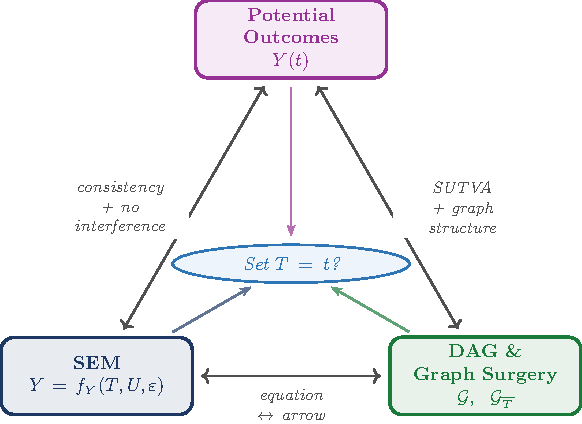
\includegraphics[keepaspectratio]{chapter_01_files/figure-pdf/fig-trinity-1.pdf}}

}

\caption{\label{fig-trinity}The \textbf{causal trinity}: three languages
that express the same causal question from different vantage points.
Potential outcomes define \emph{what} we want to estimate; the DAG with
graph surgery specifies \emph{how} to identify it; the SEM provides the
\emph{generative mechanism} for likelihood construction.}

\end{figure}%

\subsection{Language 1: Structural Equation
Models}\label{language-1-structural-equation-models}

\begin{tcolorbox}[enhanced jigsaw, arc=.35mm, bottomrule=.15mm, bottomtitle=1mm, breakable, colback=white, colbacktitle=quarto-callout-note-color!10!white, colframe=quarto-callout-note-color-frame, coltitle=black, left=2mm, leftrule=.75mm, opacityback=0, opacitybacktitle=0.6, rightrule=.15mm, title={Definition: Structural Equation Model (SEM)}, titlerule=0mm, toprule=.15mm, toptitle=1mm]

A recursive SEM over variables \((U, T, Y)\) is a system
\[U \sim p(u), \qquad T = f_T(U, \delta), \qquad Y = f_Y(T, U, \varepsilon),\]
where \(\delta\) and \(\varepsilon\) are mutually independent exogenous
disturbances and \(U\) is a confounding factor.

\end{tcolorbox}

\begin{tcolorbox}[enhanced jigsaw, arc=.35mm, bottomrule=.15mm, bottomtitle=1mm, breakable, colback=white, colbacktitle=quarto-callout-note-color!10!white, colframe=quarto-callout-note-color-frame, coltitle=black, left=2mm, leftrule=.75mm, opacityback=0, opacitybacktitle=0.6, rightrule=.15mm, title={Remark: Error Independence in the NPSEM-IE}, titlerule=0mm, toprule=.15mm, toptitle=1mm]

The assumption that \(\delta\) and \(\varepsilon\) are mutually
independent is a substantive restriction. Because \(U\) is unobserved
and enters both \(f_T\) and \(f_Y\), error independence does not remove
the dependence between \(T\) and \(Y(t)\) induced by \(U\); it restricts
only the additional channel of dependence running through the
equation-specific errors. Richardson and Robins (2014) call SEMs with
this structure \emph{Nonparametric Structural Equation Models with
Independent Errors} (NPSEM-IEs).

These notes adopt the NPSEM-IE framework throughout: error independence
ensures the DAG's Markov condition holds, making the Markov
factorization of the joint density immediate.

\end{tcolorbox}

\textbf{Observational regime.} \(T\) is determined by \(f_T\); because
\(U\) enters both \(f_T\) and \(f_Y\), we have
\(\mathrm{Cov}(T,\varepsilon) \neq 0\) in general: this is endogeneity.

\textbf{Interventional regime.} The do-operator replaces the equation
for \(T\) with a constant \(t\), yielding the \emph{mutilated system}:
\[U \sim p(u), \qquad T = t \text{ (fixed)}, \qquad Y = f_Y(t, U, \varepsilon).\]
We define the \emph{potential outcome} as
\(Y(t) \coloneqq f_Y(t, U, \varepsilon)\); by construction,
\(Y(t) \sim f(y \mid \doop(T{=}t))\).

\subsection{Language 2: Directed Acyclic
Graphs}\label{language-2-directed-acyclic-graphs}

\begin{tcolorbox}[enhanced jigsaw, arc=.35mm, bottomrule=.15mm, bottomtitle=1mm, breakable, colback=white, colbacktitle=quarto-callout-note-color!10!white, colframe=quarto-callout-note-color-frame, coltitle=black, left=2mm, leftrule=.75mm, opacityback=0, opacitybacktitle=0.6, rightrule=.15mm, title={Definition: Graph Surgery}, titlerule=0mm, toprule=.15mm, toptitle=1mm]

In the observational DAG, arrows into \(T\) encode the mechanisms that
determine \(T\). Under \(\doop(T{=}t)\), all arrows into \(T\) are
\emph{deleted}. The resulting mutilated graph \(\Gcal_T\) has no
back-door paths from \(T\) to \(Y\): the causal effect flows only along
the direct path \(T \to Y\).

\end{tcolorbox}

\subsection{Language 3: Potential
Outcomes}\label{language-3-potential-outcomes}

\begin{tcolorbox}[enhanced jigsaw, arc=.35mm, bottomrule=.15mm, bottomtitle=1mm, breakable, colback=white, colbacktitle=quarto-callout-note-color!10!white, colframe=quarto-callout-note-color-frame, coltitle=black, left=2mm, leftrule=.75mm, opacityback=0, opacitybacktitle=0.6, rightrule=.15mm, title={Definition: Potential Outcome}, titlerule=0mm, toprule=.15mm, toptitle=1mm]

(Rubin 1974) In the SEM framework, \(Y(t) = f_Y(t, U, \varepsilon)\) is
the solution for \(Y\) in the mutilated system; it is the outcome that
\emph{would have been observed} had \(T\) been set to \(t\), possibly
contrary to fact.

\textbf{SUTVA} (stable unit treatment value assumption):
\(Y_i = Y_i(T_i)\), i.e., the observed outcome for unit \(i\) equals the
potential outcome at the actual treatment received. This rules out
interference between units and multiple versions of treatment.

\end{tcolorbox}

\subsection{Roadmap: How the Trinity Organizes These
Notes}\label{roadmap-how-the-trinity-organizes-these-notes}

\textbf{Part I --- Foundations: the language of DAGs.} DAGs and the
do-operator are the primary language here because they make the
interventional/observational distinction \emph{syntactically explicit}:
confounding is visible as an open back-door path, and identifying
assumptions are visible as graph criteria.

\textbf{Part II --- Identification: bridging DAGs and observed data.}
Ignorability (\(Y(t) \indep T \mid X\)) is the potential-outcomes
counterpart of the back-door criterion; the propensity score
\(\pi(X) = P(T{=}1 \mid X)\) operationalizes it in observed data.

\textbf{Part III --- Estimation: semiparametric and machine-learning
methods.} The semiparametric efficiency framework --- efficient
influence functions, doubly robust estimators, double machine learning
--- is largely language-neutral.

\subsection{Historical Roots of the Causal Trinity}\label{sec-history}

\begin{figure}

\centering{

\pandocbounded{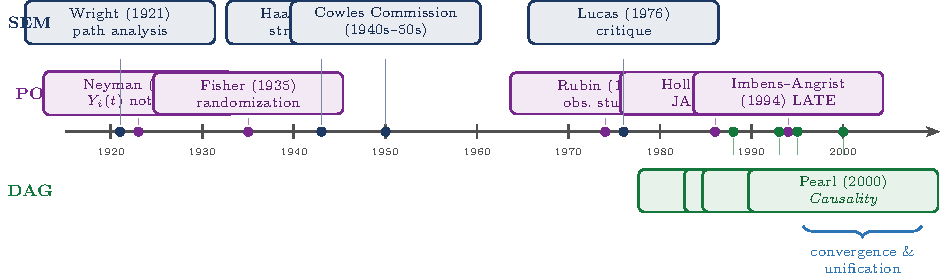
\includegraphics[keepaspectratio]{chapter_01_files/figure-pdf/fig-timeline-1.pdf}}

}

\caption{\label{fig-timeline}Key milestones in the three schools of
causal inference. SEM (top, blue) originates in genetics and
econometrics; PO (middle, purple) in experimental statistics; DAG
(bottom, green) in computer science and philosophy.}

\end{figure}%

\section{The Core Distinction}\label{sec-core}

We work within the SEM, now augmented with an observed exogenous
variable \(X\):

\begin{equation}\protect\phantomsection\label{eq-sem-core}{T = f_T(X, U, \delta), \qquad Y = f_Y(T, X, U, \varepsilon).}\end{equation}

The single most important inequality of this course is:

\begin{equation}\protect\phantomsection\label{eq-core}{\underbrace{f\!\left(y \mid x,\, \doop(T{=}t)\right)}_{\text{interventional}} \;\neq\; \underbrace{f\!\left(y \mid x,\, T{=}t\right)}_{\text{observational}} \qquad \text{whenever } T \text{ is endogenous.}}\end{equation}

\begin{tcolorbox}[enhanced jigsaw, arc=.35mm, bottomrule=.15mm, bottomtitle=1mm, breakable, colback=white, colbacktitle=quarto-callout-note-color!10!white, colframe=quarto-callout-note-color-frame, coltitle=black, left=2mm, leftrule=.75mm, opacityback=0, opacitybacktitle=0.6, rightrule=.15mm, title={Definition: Conditional Exchangeability}, titlerule=0mm, toprule=.15mm, toptitle=1mm]

Given observed covariates \(X\) and confounders \(U\), the treatment
assignment is \emph{conditionally exchangeable with the intervention} if
\(Y(t) \indep T \mid X,\, U\), or equivalently,
\[f(y \mid x,\, T{=}t,\, U{=}u) \;=\; f(y \mid x,\, \doop(T{=}t),\, U{=}u).\]
This says that once we condition on all common causes \((X, U)\) of
\(T\) and \(Y\), observing \(T{=}t\) and intervening to set \(T{=}t\)
produce the same distribution of \(Y\).

\end{tcolorbox}

\begin{tcolorbox}[enhanced jigsaw, arc=.35mm, bottomrule=.15mm, bottomtitle=1mm, breakable, colback=white, colbacktitle=quarto-callout-note-color!10!white, colframe=quarto-callout-note-color-frame, coltitle=black, left=2mm, leftrule=.75mm, opacityback=0, opacitybacktitle=0.6, rightrule=.15mm, title={Definition: Positivity}, titlerule=0mm, toprule=.15mm, toptitle=1mm]

The treatment assignment satisfies \emph{positivity} if, for all \(t\)
in the support of \(T\) and almost all \((x, u)\):
\[p(T{=}t \mid X{=}x,\, U{=}u) \;>\; 0.\]

\end{tcolorbox}

\begin{tcolorbox}[enhanced jigsaw, arc=.35mm, bottomrule=.15mm, bottomtitle=1mm, breakable, colback=white, colbacktitle=quarto-callout-tip-color!10!white, colframe=quarto-callout-tip-color-frame, coltitle=black, left=2mm, leftrule=.75mm, opacityback=0, opacitybacktitle=0.6, rightrule=.15mm, title={Proposition: Back-Door Adjustment Formula}, titlerule=0mm, toprule=.15mm, toptitle=1mm]

Under conditional exchangeability and positivity,
\[f(y \mid x,\, \doop(T{=}t)) \;=\; \int f(y \mid x,\, T{=}t,\, U{=}u)\; p(u \mid x)\; du.\]

\end{tcolorbox}

\begin{tcolorbox}[enhanced jigsaw, arc=.35mm, bottomrule=.15mm, bottomtitle=1mm, breakable, colback=white, colbacktitle=quarto-callout-note-color!10!white, colframe=quarto-callout-note-color-frame, coltitle=black, left=2mm, leftrule=.75mm, opacityback=0, opacitybacktitle=0.6, rightrule=.15mm, title={Proof}, titlerule=0mm, toprule=.15mm, toptitle=1mm]

By positivity, \(f(y \mid x,\, T{=}t,\, U{=}u)\) is well-defined. By the
law of total probability:
\[f(y \mid x,\, \doop(T{=}t)) = \int f(y \mid x,\, U{=}u,\, \doop(T{=}t))\; p(u \mid x)\; du.\]
The weight is \(p(u \mid x)\), not \(p(u \mid x, T{=}t)\), because under
\(\doop(T{=}t)\) the treatment carries no information about \(U\). By
conditional exchangeability,
\(f(y \mid x,\, U{=}u,\, \doop(T{=}t)) = f(y \mid x,\, T{=}t,\, U{=}u)\).
\(\square\)

\end{tcolorbox}

\begin{tcolorbox}[enhanced jigsaw, arc=.35mm, bottomrule=.15mm, bottomtitle=1mm, breakable, colback=white, colbacktitle=quarto-callout-note-color!10!white, colframe=quarto-callout-note-color-frame, coltitle=black, left=2mm, leftrule=.75mm, opacityback=0, opacitybacktitle=0.6, rightrule=.15mm, title={Remark: Confounding Discrepancy}, titlerule=0mm, toprule=.15mm, toptitle=1mm]

What OLS estimates is the observational density, not the interventional
density:
\[f(y \mid x,\, T{=}t) = \int f(y \mid x,\, T{=}t,\, U{=}u)\; p(u \mid x,\, T{=}t)\; du.\]
The kernel is the same as in Equation~\ref{eq-backdoor-cont}, but
averaged over the \emph{selection-distorted} weight
\(p(u \mid x, T{=}t)\). Because \(U\) and \(T\) are dependent through
the back-door path, \(p(u \mid x, T{=}t) \neq p(u \mid x)\), and the gap
is non-zero whenever \(T\) is endogenous.

\end{tcolorbox}

\subsection{Two Scenarios: Observed vs.~Unobserved
Confounder}\label{two-scenarios-observed-vs.-unobserved-confounder}

{\def\LTcaptype{none} % do not increment counter
\begin{longtable}[]{@{}
  >{\raggedright\arraybackslash}p{(\linewidth - 4\tabcolsep) * \real{0.3333}}
  >{\raggedright\arraybackslash}p{(\linewidth - 4\tabcolsep) * \real{0.3333}}
  >{\raggedright\arraybackslash}p{(\linewidth - 4\tabcolsep) * \real{0.3333}}@{}}
\toprule\noalign{}
\begin{minipage}[b]{\linewidth}\raggedright
\end{minipage} & \begin{minipage}[b]{\linewidth}\raggedright
\textbf{Scenario 1: \(U\) observed}
\end{minipage} & \begin{minipage}[b]{\linewidth}\raggedright
\textbf{Scenario 2: \(U\) unobserved}
\end{minipage} \\
\midrule\noalign{}
\endhead
\bottomrule\noalign{}
\endlastfoot
Confounding type & No unmeasured confounding & Unmeasured confounding \\
Back-door formula usable? & Yes & No: \(U\) latent \\
Identification route & Back-door adjustment / standardization & IV,
front-door, \ldots{} \\
Key assumption & Unconfoundedness: \(U \indep T \mid X\) & Exclusion
restriction, monotonicity, \ldots{} \\
Chapters in this course & Chapters 2--6 & Chapter 7 \\
\end{longtable}
}

\textbf{Scenario 1: \(U\) is observed.} The back-door adjustment formula
Equation~\ref{eq-backdoor-cont} is usable from data:

\begin{equation}\protect\phantomsection\label{eq-backdoor-cont}{f(y \mid x,\, \doop(T{=}t)) = \int f(y \mid x,\, T{=}t,\, U{=}u)\; p(u \mid x)\; du.}\end{equation}

A special case is \emph{unconfoundedness}: if \(U \indep T \mid X\)
already holds observationally, Equation~\ref{eq-backdoor-cont} reduces
to the familiar regression \(\E[Y \mid X{=}x, T{=}t]\).

\textbf{Scenario 2: \(U\) is unobserved.}
Equation~\ref{eq-backdoor-cont} is not usable. Additional structure
beyond \((Y, T, X)\) must be imposed: \textbf{instrumental variables}
(Chapter 7), the \textbf{front-door criterion} (Chapter 3), or
\textbf{sensitivity analysis}.

\section{The Gaussian Linear Confounded Model}\label{sec-gaussian}

\subsection{Setup}\label{setup}

\begin{tcolorbox}[enhanced jigsaw, arc=.35mm, bottomrule=.15mm, bottomtitle=1mm, breakable, colback=white, colbacktitle=quarto-callout-note-color!10!white, colframe=quarto-callout-note-color-frame, coltitle=black, left=2mm, leftrule=.75mm, opacityback=0, opacitybacktitle=0.6, rightrule=.15mm, title={Example: Gaussian Linear Confounded Model}, titlerule=0mm, toprule=.15mm, toptitle=1mm]

The structural equations are

\begin{equation}\protect\phantomsection\label{eq-iv}{Y = \beta T + \gamma U + \varepsilon, \qquad T = \alpha U + \delta,}\end{equation}

where \(U\) is an unobserved confounder and the three primitive
variables are mutually independent:
\(U \sim \mathcal{N}(0,\sigma_U^2)\),
\(\varepsilon \sim \mathcal{N}(0,\sigma_\varepsilon^2)\),
\(\delta \sim \mathcal{N}(0,\sigma_\delta^2)\).

Here \(\beta\) is the causal effect of \(T\) on \(Y\), \(\gamma\) is the
direct effect of \(U\) on \(Y\), and \(\alpha\) is the direct effect of
\(U\) on \(T\).

\end{tcolorbox}

The endogeneity of \(T\) is immediate:
\(\mathrm{Cov}(T,\, \gamma U + \varepsilon) = \gamma\alpha\sigma_U^2 \neq 0\)
when \(\alpha \neq 0\) and \(\gamma \neq 0\). Consequently, OLS
regressing \(Y\) on \(T\) does not estimate \(\beta\).

\begin{figure}

\centering{

\pandocbounded{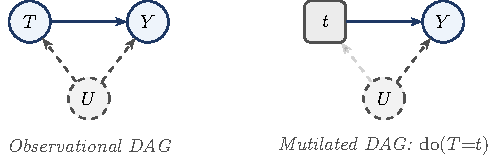
\includegraphics[keepaspectratio]{chapter_01_files/figure-pdf/fig-surgery-1.pdf}}

}

\caption{\label{fig-surgery}Graph surgery on the Gaussian confounded
model. The faded arrow in the mutilated DAG has been severed by the
intervention \(\doop(T{=}t)\). The back-door path
\(T \leftarrow U \to Y\) is eliminated; only the causal path \(T \to Y\)
remains active.}

\end{figure}%

\subsection{Two Explicit Densities}\label{two-explicit-densities}

Write \(\sigma_T^2 = \alpha^2\sigma_U^2 + \sigma_\delta^2\) for the
marginal variance of \(T\).

\textbf{Interventional density.} Set \(T = t\) externally. \(U\) is
drawn from its marginal \(\mathcal{N}(0,\sigma_U^2)\) independently.
Hence

\begin{equation}\protect\phantomsection\label{eq-int}{f\!\left(y \mid \doop(T{=}t)\right) = \mathcal{N}\!\left(\beta t,\;\; \gamma^2\sigma_U^2 + \sigma_\varepsilon^2\right).}\end{equation}

\textbf{Observational density.} Since \((Y, T)\) is jointly normal with
\(\mathrm{Cov}(Y, T) = \beta\sigma_T^2 + \gamma\alpha\sigma_U^2\), the
conditional normal formula gives:

\begin{equation}\protect\phantomsection\label{eq-obs}{f\!\left(y \mid T{=}t\right) = \mathcal{N}\!\left(\left(\beta + \frac{\gamma\alpha\sigma_U^2}{\sigma_T^2}\right)t,\;\; \frac{\gamma^2\sigma_U^2\sigma_\delta^2}{\sigma_T^2} + \sigma_\varepsilon^2\right).}\end{equation}

\subsection{The Endogeneity Gap}\label{the-endogeneity-gap}

{\def\LTcaptype{none} % do not increment counter
\begin{longtable}[]{@{}
  >{\raggedright\arraybackslash}p{(\linewidth - 4\tabcolsep) * \real{0.3333}}
  >{\raggedright\arraybackslash}p{(\linewidth - 4\tabcolsep) * \real{0.3333}}
  >{\raggedright\arraybackslash}p{(\linewidth - 4\tabcolsep) * \real{0.3333}}@{}}
\toprule\noalign{}
\begin{minipage}[b]{\linewidth}\raggedright
\end{minipage} & \begin{minipage}[b]{\linewidth}\raggedright
\textbf{Interventional}
\end{minipage} & \begin{minipage}[b]{\linewidth}\raggedright
\textbf{Observational}
\end{minipage} \\
\midrule\noalign{}
\endhead
\bottomrule\noalign{}
\endlastfoot
Mean & \(\beta t\) &
\(\left(\beta + \frac{\gamma\alpha\sigma_U^2}{\sigma_T^2}\right)t\) \\
Variance & \(\gamma^2\sigma_U^2 + \sigma_\varepsilon^2\) &
\(\frac{\gamma^2\sigma_U^2\sigma_\delta^2}{\sigma_T^2} + \sigma_\varepsilon^2\) \\
Residual & \((\gamma U{+}\varepsilon) \indep T\) &
\((\gamma U{+}\varepsilon)\) correlated with \(T\) \\
Identified by & RCT (or IV, Chapter 7) & OLS \\
\end{longtable}
}

The \emph{endogeneity bias} of OLS is
\(\gamma\alpha\sigma_U^2/\sigma_T^2\). Numerically, with
\(\alpha = \gamma = 1\) and \(\sigma_U^2 = \sigma_\delta^2 = 1\): bias
\(= 1/2 = 0.5\).

\subsection{Lab: Simulating the Two
Densities}\label{lab-simulating-the-two-densities}

The analytical results were verified by simulation using
\(n = 10{,}000\) draws with parameters \(\beta = 2\), \(\alpha = 1\),
\(\gamma = 1\), \(\sigma_U = \sigma_\varepsilon = \sigma_\delta = 1\).

\textbf{Experiment 1: OLS bias.}

{\def\LTcaptype{none} % do not increment counter
\begin{longtable}[]{@{}
  >{\raggedright\arraybackslash}p{(\linewidth - 6\tabcolsep) * \real{0.2500}}
  >{\raggedright\arraybackslash}p{(\linewidth - 6\tabcolsep) * \real{0.2500}}
  >{\raggedright\arraybackslash}p{(\linewidth - 6\tabcolsep) * \real{0.2500}}
  >{\raggedright\arraybackslash}p{(\linewidth - 6\tabcolsep) * \real{0.2500}}@{}}
\toprule\noalign{}
\begin{minipage}[b]{\linewidth}\raggedright
\end{minipage} & \begin{minipage}[b]{\linewidth}\raggedright
\textbf{Simulated}
\end{minipage} & \begin{minipage}[b]{\linewidth}\raggedright
\textbf{Theory}
\end{minipage} & \begin{minipage}[b]{\linewidth}\raggedright
\textbf{Formula}
\end{minipage} \\
\midrule\noalign{}
\endhead
\bottomrule\noalign{}
\endlastfoot
OLS slope & 2.5147 & 2.5000 &
\(\beta + \gamma\alpha\sigma_U^2/\sigma_T^2\) \\
True \(\beta\) & --- & 2.0000 & \(\beta\) \\
Bias & 0.5147 & 0.5000 & \(\gamma\alpha\sigma_U^2/\sigma_T^2\) \\
\end{longtable}
}

\textbf{Experiment 2: Two-sample comparison at \(t_0 = 1\).}

{\def\LTcaptype{none} % do not increment counter
\begin{longtable}[]{@{}
  >{\raggedright\arraybackslash}p{(\linewidth - 8\tabcolsep) * \real{0.2000}}
  >{\raggedright\arraybackslash}p{(\linewidth - 8\tabcolsep) * \real{0.2000}}
  >{\raggedright\arraybackslash}p{(\linewidth - 8\tabcolsep) * \real{0.2000}}
  >{\raggedright\arraybackslash}p{(\linewidth - 8\tabcolsep) * \real{0.2000}}
  >{\raggedright\arraybackslash}p{(\linewidth - 8\tabcolsep) * \real{0.2000}}@{}}
\toprule\noalign{}
\begin{minipage}[b]{\linewidth}\raggedright
\end{minipage} & \begin{minipage}[b]{\linewidth}\raggedright
\textbf{Mean (Simulated)}
\end{minipage} & \begin{minipage}[b]{\linewidth}\raggedright
\textbf{Mean (Theory)}
\end{minipage} & \begin{minipage}[b]{\linewidth}\raggedright
\textbf{SD (Simulated)}
\end{minipage} & \begin{minipage}[b]{\linewidth}\raggedright
\textbf{SD (Theory)}
\end{minipage} \\
\midrule\noalign{}
\endhead
\bottomrule\noalign{}
\endlastfoot
\(\E[Y \mid T{=}1]\) & 2.497 & 2.500 & 1.229 & \(\sqrt{1.5} = 1.225\) \\
\(\E[Y \mid \doop(T{=}1)]\) & 2.001 & 2.000 & 1.428 &
\(\sqrt{2} = 1.414\) \\
\end{longtable}
}

\textbf{Experiment 3: Density overlay for varying \(\alpha\).}
Figure~\ref{fig-density} shows the interventional density (solid) and
the observational density Equation~\ref{eq-obs} (dashed), both evaluated
at \(t_0 = 1\), for \(\alpha \in \{0, 0.3, 0.7, 1.0\}\).

\begin{figure}

\centering{

\pandocbounded{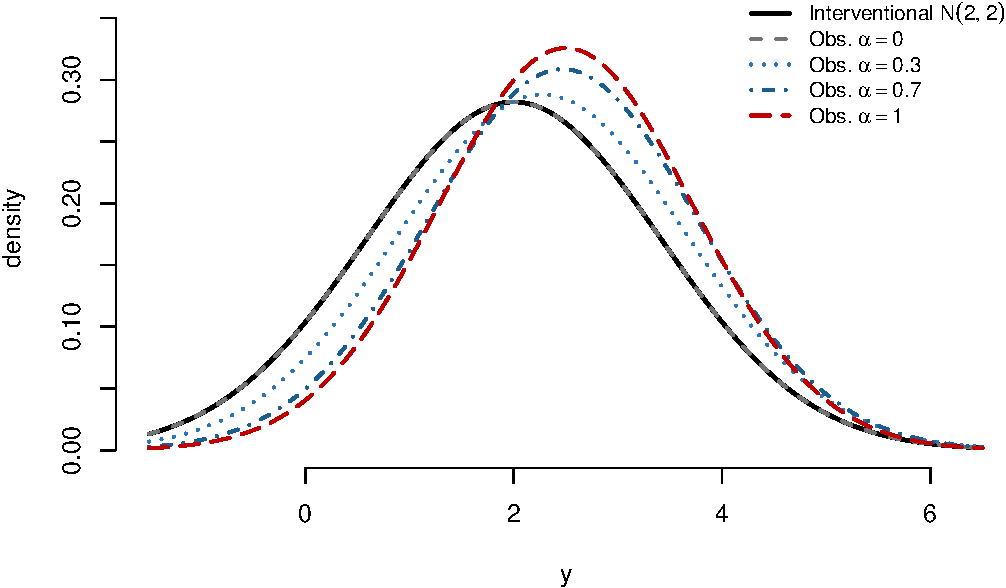
\includegraphics[keepaspectratio]{chapter_01_files/figure-pdf/fig-density-1.pdf}}

}

\caption{\label{fig-density}Interventional density \(\mathcal{N}(2,2)\)
(solid black) versus observational density for
\(\alpha \in \{0, 0.3, 0.7, 1.0\}\) (dashed), evaluated at \(t_0 = 1\).
As \(\alpha\) increases, the observational curve shifts rightward
(growing bias) and narrows (reduced variance).}

\end{figure}%

\section{The Two-Step Paradigm}\label{sec-two-step}

Causal inference is a two-step discipline. The two steps are logically
distinct and require different tools.

\subsection{Step 1: Identification}\label{step-1-identification}

\begin{tcolorbox}[enhanced jigsaw, arc=.35mm, bottomrule=.15mm, bottomtitle=1mm, breakable, colback=white, colbacktitle=quarto-callout-note-color!10!white, colframe=quarto-callout-note-color-frame, coltitle=black, left=2mm, leftrule=.75mm, opacityback=0, opacitybacktitle=0.6, rightrule=.15mm, title={Definition: Identification}, titlerule=0mm, toprule=.15mm, toptitle=1mm]

A causal quantity \(P(y \mid \doop(T{=}t))\) is \emph{identified} from
the observational distribution \(P\) if there exists a functional
\(\Psi\) such that \(P(y \mid \doop(T{=}t)) = \Psi(P)\), and \(\Psi(P)\)
depends only on the observable joint distribution.

\end{tcolorbox}

Identification is a purely mathematical question about the structure of
the causal model: given the assumed graph and assumptions, can the
interventional density be expressed as a function of the observed-data
distribution? It does not depend on sample size.

The main tools are the back-door criterion (Chapters 2--3, applied in
Chapters 5--6), the front-door criterion (Chapter 3), the three rules of
the do-calculus (Chapter 3), and IV assumptions (Chapter 7).

\subsection{Step 2: Estimation}\label{step-2-estimation}

Once \(\Psi(P)\) has been identified, the statistical problem is to
estimate \(\Psi(P)\) from \(n\) observations \(O_1,\dots,O_n\) as
efficiently as possible. The main tools are efficient influence
functions (EIF), inverse probability weighting (IPW), doubly robust
estimators, and double machine learning (DML), all covered in Part III.

\subsection{A Worked Example: Flu Vaccination and
Infection}\label{sec-simpson}

\textbf{Scenario.} A public health agency observes 1,000 individuals
over one flu season. Each person either received a flu vaccine (\(T=1\))
or did not (\(T=0\)), and either became infected (\(Y=1\)) or did not
(\(Y=0\)). Age group \(X\) (elderly \(= E\), young \(= Y\)) is recorded
for all individuals. Elderly people are more likely to be vaccinated and
more susceptible to infection, so \(X\) confounds the relationship
between \(T\) and \(Y\).

\begin{figure}

\centering{

\pandocbounded{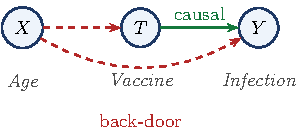
\includegraphics[keepaspectratio]{chapter_01_files/figure-pdf/fig-vaccination-1.pdf}}

}

\caption{\label{fig-vaccination}Causal DAG for the vaccination example.
The green arrow is the causal path \(T \to Y\). The red dashed arrows
form the back-door path \(T \leftarrow X \to Y\).}

\end{figure}%

\textbf{Observed data.}

{\def\LTcaptype{none} % do not increment counter
\begin{longtable}[]{@{}llllll@{}}
\toprule\noalign{}
& \textbf{Vaccinated (\(T=1\))} & & \textbf{Unvaccinated (\(T=0\))} & &
Total \\
\midrule\noalign{}
\endhead
\bottomrule\noalign{}
\endlastfoot
& \(n\) & Infected & \(n\) & Infected & \\
Elderly (\(X=E\)) & 360 & 108 (30\%) & 40 & 20 (50\%) & 400 \\
Young (\(X=Y\)) & 60 & 3 (5\%) & 540 & 54 (10\%) & 600 \\
\textbf{Total} & 420 & 111 (26.4\%) & 580 & 74 (12.8\%) & 1,000 \\
\end{longtable}
}

\textbf{Simpson's paradox.}

{\def\LTcaptype{none} % do not increment counter
\begin{longtable}[]{@{}
  >{\raggedright\arraybackslash}p{(\linewidth - 8\tabcolsep) * \real{0.2000}}
  >{\raggedright\arraybackslash}p{(\linewidth - 8\tabcolsep) * \real{0.2000}}
  >{\raggedright\arraybackslash}p{(\linewidth - 8\tabcolsep) * \real{0.2000}}
  >{\raggedright\arraybackslash}p{(\linewidth - 8\tabcolsep) * \real{0.2000}}
  >{\raggedright\arraybackslash}p{(\linewidth - 8\tabcolsep) * \real{0.2000}}@{}}
\toprule\noalign{}
\begin{minipage}[b]{\linewidth}\raggedright
\textbf{Stratum}
\end{minipage} & \begin{minipage}[b]{\linewidth}\raggedright
\textbf{Vaccinated}
\end{minipage} & \begin{minipage}[b]{\linewidth}\raggedright
\textbf{Unvaccinated}
\end{minipage} & \begin{minipage}[b]{\linewidth}\raggedright
\textbf{Difference}
\end{minipage} & \begin{minipage}[b]{\linewidth}\raggedright
\textbf{Conclusion}
\end{minipage} \\
\midrule\noalign{}
\endhead
\bottomrule\noalign{}
\endlastfoot
Elderly (\(X=E\)) & 30\% & 50\% & \(-20\) pp & vaccine helps \\
Young (\(X=Y\)) & 5\% & 10\% & \(-5\) pp & vaccine helps \\
\textbf{Aggregate (raw)} & \textbf{26.4\%} & \textbf{12.8\%} & \(+13.6\)
pp & \textbf{vaccine harms??} \\
\end{longtable}
}

Within every stratum the vaccine reduces infection. The reversal occurs
because the vaccinated group is disproportionately elderly (86\%
vs.~7\%).

\textbf{Step 1: Identification.} The set \(\{X\}\) satisfies the
back-door criterion. By the back-door formula:

\begin{equation}\protect\phantomsection\label{eq-backdoor}{P\!\left(Y{=}1 \mid \doop(T{=}t)\right) = \sum_{x \in \{E,Y\}} P(Y{=}1 \mid T{=}t, X{=}x)\,P(X{=}x).}\end{equation}

\textbf{Step 2: Estimation.}
\[\hat{P}(Y{=}1 \mid \doop(T{=}1)) = 0.30 \times 0.4 + 0.05 \times 0.6 = 0.15,\]
\[\hat{P}(Y{=}1 \mid \doop(T{=}0)) = 0.50 \times 0.4 + 0.10 \times 0.6 = 0.26.\]
The estimated causal risk difference is
\(\hat{\Delta}_{\mathrm{causal}} = 0.15 - 0.26 = -0.11\): the vaccine
causally reduces infection probability by 11 percentage points.

\begin{tcolorbox}[enhanced jigsaw, arc=.35mm, bottomrule=.15mm, bottomtitle=1mm, breakable, colback=white, colbacktitle=quarto-callout-note-color!10!white, colframe=quarto-callout-note-color-frame, coltitle=black, left=2mm, leftrule=.75mm, opacityback=0, opacitybacktitle=0.6, rightrule=.15mm, title={The Two Steps, Concretely}, titlerule=0mm, toprule=.15mm, toptitle=1mm]

\textbf{Step 1 (identification)} established --- from the DAG alone ---
that the back-door formula Equation~\ref{eq-backdoor} expresses the
causal quantity as a functional of observable data. \textbf{Step 2
(estimation)} replaced the population probabilities with sample
proportions.

These two steps are logically separate: Step 1 is a mathematical
argument about the causal model that does not depend on sample size;
Step 2 is a statistical argument about finite-sample estimation that
does not depend on the causal model.

\end{tcolorbox}

\section{Summary}\label{summary}

\begin{enumerate}
\def\labelenumi{\arabic{enumi}.}
\item
  \textbf{Interventional vs.~observational distribution.} Causal
  inference answers questions about interventions
  \(f(y \mid \doop(T{=}t))\), not about observations
  \(f(y \mid T{=}t)\). These two distributions coincide only under
  exogeneity; whenever \(T\) is endogenous they differ, and the
  difference is endogeneity bias.
\item
  \textbf{The causal trinity.} The same causal question can be expressed
  in three languages --- SEM (equation surgery), DAG (graph surgery),
  and potential outcomes (\(Y(t)\)). In the SEM framework, \(Y(t)\) is
  defined as the solution for \(Y\) in the mutilated system, so
  \(Y(t) \sim f(y \mid \doop(T{=}t))\) by construction. Fluency in all
  three is essential for modern causal reasoning.
\item
  \textbf{Endogeneity bias in the Gaussian confounded model.} In the
  Gaussian linear confounded model, the coefficient of \(T\) in the
  observational mean \(\E[Y \mid T{=}t]\) differs from the causal
  coefficient \(\beta\) by \(\gamma\alpha\sigma_U^2/\sigma_T^2\), where
  \(\sigma_T^2 = \alpha^2\sigma_U^2 + \sigma_\delta^2\). This is the
  omitted-variable bias.
\item
  \textbf{Two-step paradigm.} Causal inference is a two-step discipline:
  \emph{identification} (expressing \(\Psi(P)\) as a functional of
  observable data, a mathematical question about the causal model)
  followed by \emph{estimation} (constructing \(\hat{\Psi}_n\)
  efficiently from \(n\) observations, a statistical question about
  finite samples). The two steps are logically independent.
\end{enumerate}

\emph{Causal inference is the study of when the observational
distribution contains enough information to recover the interventional
distribution.} Everything in this course --- the back-door criterion,
do-calculus, instrumental variables, doubly robust estimation --- is an
answer to that question in a particular setting.

\section{Problems}\label{problems}

\textbf{1. Do-notation fundamentals.} For each statement below, decide
whether it refers to an interventional or an observational distribution,
and rewrite it unambiguously using do-notation where appropriate.

\begin{enumerate}
\def\labelenumi{(\alph{enumi})}
\tightlist
\item
  ``The probability that a patient recovers given that they took the
  drug.''
\item
  ``The probability that a patient would recover if we prescribed the
  drug to everyone.''
\item
  ``Among students who attended tutoring, the average exam score was
  85.''
\item
  ``If we enrolled all students in tutoring, the average exam score
  would be 85.''
\end{enumerate}

\textbf{2. Deriving the observational density.} In the Gaussian
confounded model, verify Equation~\ref{eq-obs} by carrying out the
following steps. Let
\(\sigma_T^2 = \alpha^2\sigma_U^2 + \sigma_\delta^2\).

\begin{enumerate}
\def\labelenumi{(\alph{enumi})}
\tightlist
\item
  Show that \((Y, T)\) is jointly normal by writing both as linear
  combinations of the independent normals \((U, \varepsilon, \delta)\).
\item
  Compute \(\mathrm{Cov}(Y, T)\) and \(\mathrm{Var}(T)\).
\item
  Apply the conditional normal formula to derive \(\E[Y \mid T{=}t]\)
  and \(\mathrm{Var}[Y \mid T{=}t]\), and hence verify
  Equation~\ref{eq-obs}.
\item
  Show that the OLS probability limit is
  \(\beta + \gamma\alpha\sigma_U^2/\sigma_T^2\), and interpret this as
  an omitted-variable bias formula.
\end{enumerate}

\textbf{3. The causal trinity.} Consider the following verbal causal
claim: ``Aspirin (\(T\)) reduces the risk of heart attack (\(Y\))
because it inhibits platelet aggregation (\(M\)), but patients with
pre-existing cardiovascular disease (\(U\), unobserved) are both more
likely to take aspirin and more likely to have a heart attack.''

\begin{enumerate}
\def\labelenumi{(\alph{enumi})}
\tightlist
\item
  Draw the causal DAG implied by this description.
\item
  Write down the recursive SEM with appropriate structural functions
  \(f_T\), \(f_M\), \(f_Y\).
\item
  State the SUTVA assumption and discuss whether it is plausible in this
  setting.
\item
  Explain why \(\E[Y \mid T{=}1] - \E[Y \mid T{=}0]\) does not identify
  the causal effect
  \(\E[Y \mid \doop(T{=}1)] - \E[Y \mid \doop(T{=}0)]\) in this DAG.
\end{enumerate}

\bookmarksetup{startatroot}

\chapter{DAGs and d-Separation}\label{dags-and-d-separation}

\begin{tcolorbox}[enhanced jigsaw, arc=.35mm, bottomrule=.15mm, bottomtitle=1mm, breakable, colback=white, colbacktitle=quarto-callout-note-color!10!white, colframe=quarto-callout-note-color-frame, coltitle=black, left=2mm, leftrule=.75mm, opacityback=0, opacitybacktitle=0.6, rightrule=.15mm, title={Learning Objectives}, titlerule=0mm, toprule=.15mm, toptitle=1mm]

By the end of this chapter, students should be able to:

\begin{enumerate}
\def\labelenumi{\arabic{enumi}.}
\tightlist
\item
  Construct a DAG from a verbal description of a causal model and
  identify parents, descendants, ancestors, and non-descendants of any
  node.
\item
  Classify every intermediate node on a path as a chain, fork, or
  collider, and apply the blocking rule for each.
\item
  Apply the d-separation criterion to determine all conditional
  independence relationships implied by a DAG.
\item
  Recognize and avoid collider bias, including the case where a
  descendant of a collider is conditioned upon.
\item
  State the Markov factorization and use it to write the joint density
  of a DAG in terms of local conditional densities.
\item
  Interpret d-separation results as conditional independence assumptions
  on observed variables, and recognize their role as the graphical
  expression of causal assumptions.
\end{enumerate}

\end{tcolorbox}

\section{Directed Acyclic Graphs}\label{directed-acyclic-graphs}

DAGs allow us to translate qualitative causal assumptions into
quantitative statistical restrictions. This single idea underlies
everything in this chapter: once we draw a graph encoding what we
believe about the causal structure of a problem, the graph tells us
exactly which variables are independent, which are confounded, and what
we need to condition on to identify a causal effect.

\begin{tcolorbox}[enhanced jigsaw, arc=.35mm, bottomrule=.15mm, bottomtitle=1mm, breakable, colback=white, colbacktitle=quarto-callout-note-color!10!white, colframe=quarto-callout-note-color-frame, coltitle=black, left=2mm, leftrule=.75mm, opacityback=0, opacitybacktitle=0.6, rightrule=.15mm, title={Remark}, titlerule=0mm, toprule=.15mm, toptitle=1mm]

In this chapter, the word \emph{graph} does not mean a plot of data or a
graph of a function. It means a collection of nodes and edges used to
represent relationships among variables. Our objective is to understand
how such graphs encode statistical structure --- especially conditional
independence, confounding, and path blocking --- and how this graphical
structure will later support causal identification.

\end{tcolorbox}

\subsection{Basic Definition}\label{basic-definition}

\begin{tcolorbox}[enhanced jigsaw, arc=.35mm, bottomrule=.15mm, bottomtitle=1mm, breakable, colback=white, colbacktitle=quarto-callout-note-color!10!white, colframe=quarto-callout-note-color-frame, coltitle=black, left=2mm, leftrule=.75mm, opacityback=0, opacitybacktitle=0.6, rightrule=.15mm, title={Definition: Directed Acyclic Graph}, titlerule=0mm, toprule=.15mm, toptitle=1mm]

A \emph{directed acyclic graph} (DAG) \(\Gcal = (V, E)\) consists of a
finite set of nodes \(V\) and a set of directed edges
\(E \subseteq V \times V\) such that there is no directed cycle: no node
\(V_i\) has a directed path to itself.

\end{tcolorbox}

In a causal DAG each node represents a variable and each directed edge
\(A \to B\) encodes ``\(A\) is a direct cause of \(B\), given all other
variables in the model.'' The acyclicity condition is essential: it
guarantees that the variables can be ordered topologically so that the
joint density admits the recursive factorization
\[p(v_1,\dots,v_k) = \prod_{i=1}^{k} p(v_i \mid \Pa(v_i)).\]

\subsection{Structural Relationships}\label{structural-relationships}

\begin{tcolorbox}[enhanced jigsaw, arc=.35mm, bottomrule=.15mm, bottomtitle=1mm, breakable, colback=white, colbacktitle=quarto-callout-note-color!10!white, colframe=quarto-callout-note-color-frame, coltitle=black, left=2mm, leftrule=.75mm, opacityback=0, opacitybacktitle=0.6, rightrule=.15mm, title={Definition: Structural Relationships in a DAG}, titlerule=0mm, toprule=.15mm, toptitle=1mm]

For a node \(v \in \mathcal{V}\) in \(\Gcal = (\mathcal{V}, E)\):

\begin{itemize}
\tightlist
\item
  \(\Pa(v) = \{w \in \mathcal{V} : w \to v \in E\}\) are the
  \emph{parents} of \(v\).
\item
  \(\De(v)\) = all nodes reachable from \(v\) by directed paths are the
  \emph{descendants} of \(v\).
\item
  \(\An(v)\) = all nodes with a directed path to \(v\) are the
  \emph{ancestors} of \(v\).
\item
  \(\Nd(v) = \mathcal{V} \setminus (\De(v) \cup \{v\})\) are the
  \emph{non-descendants} of \(v\).
\end{itemize}

Note that \(\Nd(v)\) includes the parents of \(v\); when stating the
local Markov property in Section~\ref{sec-markov}, we will exclude the
parents explicitly.

\end{tcolorbox}

\begin{tcolorbox}[enhanced jigsaw, arc=.35mm, bottomrule=.15mm, bottomtitle=1mm, breakable, colback=white, colbacktitle=quarto-callout-note-color!10!white, colframe=quarto-callout-note-color-frame, coltitle=black, left=2mm, leftrule=.75mm, opacityback=0, opacitybacktitle=0.6, rightrule=.15mm, title={Quick Terminology Summary}, titlerule=0mm, toprule=.15mm, toptitle=1mm]

A \emph{node} represents a variable, and an \emph{edge} represents a
relationship between two variables. If \(A \to B\), then \(A\) is a
\emph{parent} of \(B\) and \(B\) is a \emph{child} of \(A\). Two nodes
are \emph{adjacent} if they are connected by an edge. A \emph{path} is
any sequence of connected nodes, regardless of arrow direction; a
\emph{directed path} is a path whose arrows all point in the same
direction. A \emph{directed acyclic graph} (DAG) is a directed graph
with no directed cycles.

\end{tcolorbox}

\begin{tcolorbox}[enhanced jigsaw, arc=.35mm, bottomrule=.15mm, bottomtitle=1mm, breakable, colback=white, colbacktitle=quarto-callout-note-color!10!white, colframe=quarto-callout-note-color-frame, coltitle=black, left=2mm, leftrule=.75mm, opacityback=0, opacitybacktitle=0.6, rightrule=.15mm, title={Example: Education, Earnings, and Family Background}, titlerule=0mm, toprule=.15mm, toptitle=1mm]

Consider the causal story: education (\(E\)) affects earnings (\(Y\));
family background (\(B\)) is a common cause of both; and neighborhood
(\(N\)) affects education but has no direct effect on earnings.

\pandocbounded{
\includegraphics[keepaspectratio]{chapter_02_files/figure-pdf/unnamed-chunk-1-1.pdf}}

The Markov factorization is
\(p(n,b,e,y) = p(n)\,p(b)\,p(e\mid n,b)\,p(y\mid e,b)\). Reading off
structural relationships: \(\Pa(E) = \{N,B\}\), \(\Pa(Y) = \{E,B\}\),
\(\Pa(N)=\Pa(B)=\varnothing\). The descendants of \(N\) are \(\{E,Y\}\);
\(B\) and \(N\) are non-descendants of each other.

\end{tcolorbox}

\begin{tcolorbox}[enhanced jigsaw, arc=.35mm, bottomrule=.15mm, bottomtitle=1mm, breakable, colback=white, colbacktitle=quarto-callout-note-color!10!white, colframe=quarto-callout-note-color-frame, coltitle=black, left=2mm, leftrule=.75mm, opacityback=0, opacitybacktitle=0.6, rightrule=.15mm, title={Example: The IV DAG}, titlerule=0mm, toprule=.15mm, toptitle=1mm]

The canonical instrumental variable model involves four nodes: \(Z\)
(instrument), \(T\) (treatment), \(Y\) (outcome), and \(U\) (unobserved
confounder).

\pandocbounded{
\includegraphics[keepaspectratio]{chapter_02_files/figure-pdf/unnamed-chunk-2-1.pdf}}

\(\Pa(T) = \{Z,U\}\), \(\Pa(Y) = \{T,U\}\),
\(\Pa(Z) = \Pa(U) = \varnothing\). The descendants of \(Z\) are
\(\{T, Y\}\); \(U\) and \(Z\) are non-descendants of each other.

\end{tcolorbox}

\begin{tcolorbox}[enhanced jigsaw, arc=.35mm, bottomrule=.15mm, bottomtitle=1mm, breakable, colback=white, colbacktitle=quarto-callout-note-color!10!white, colframe=quarto-callout-note-color-frame, coltitle=black, left=2mm, leftrule=.75mm, opacityback=0, opacitybacktitle=0.6, rightrule=.15mm, title={Example: The Mediation DAG}, titlerule=0mm, toprule=.15mm, toptitle=1mm]

In a mediation model, treatment \(T\) affects outcome \(Y\) both
directly and through an intermediate variable \(M\) (the mediator). An
unobserved confounder \(U\) creates a back-door path
\(T \leftarrow U \rightarrow Y\), making \(T\) endogenous. The mediator
\(M\) is itself unconfounded.

\pandocbounded{
\includegraphics[keepaspectratio]{chapter_02_files/figure-pdf/unnamed-chunk-3-1.pdf}}

\(\Pa(T) = \{U\}\), \(\Pa(M) = \{T\}\), \(\Pa(Y) = \{M, T, U\}\),
\(\Pa(U) = \varnothing\). The total effect of \(T\) on \(Y\) travels
along two paths: the direct path \(T \to Y\) and the indirect path
\(T \to M \to Y\). Because there is a direct path \(T \to Y\) bypassing
\(M\), the front-door criterion does not apply here.

\end{tcolorbox}

\section{Paths, Blocking, and
d-Separation}\label{paths-blocking-and-d-separation}

A DAG encodes direct causal relationships through its edges, but
variables can also be statistically related through longer routes that
mix directed and reversed edges. The concept of a \emph{path} formalises
these routes, and the question of whether a path transmits or blocks
statistical dependence --- depending on which variables are conditioned
upon --- is precisely what d-separation answers. The key insight is that
conditioning can both \emph{close} channels that were open (by blocking
a chain or fork) and \emph{open} channels that were closed (by
activating a collider). Figure~\ref{fig-chain-fork-collider} illustrates
all three cases.

\subsection{Path Structures}\label{path-structures}

\begin{tcolorbox}[enhanced jigsaw, arc=.35mm, bottomrule=.15mm, bottomtitle=1mm, breakable, colback=white, colbacktitle=quarto-callout-note-color!10!white, colframe=quarto-callout-note-color-frame, coltitle=black, left=2mm, leftrule=.75mm, opacityback=0, opacitybacktitle=0.6, rightrule=.15mm, title={Definition: Path}, titlerule=0mm, toprule=.15mm, toptitle=1mm]

A \emph{path} between nodes \(X\) and \(Y\) in \(\Gcal\) is any sequence
of distinct nodes \(X = V_0, V_1, \dots, V_k = Y\) such that each
consecutive pair is connected by an edge in either direction.

\end{tcolorbox}

Every intermediate node \(V_m\) on a path plays one of three structural
roles. In a \textbf{chain} (\(V_{m-1} \to V_m \to V_{m+1}\)), \(V_m\) is
a causal intermediary through which influence is transmitted. In a
\textbf{fork} (\(V_{m-1} \leftarrow V_m \to V_{m+1}\)), \(V_m\) is a
common cause that creates confounding between the two endpoints. In a
\textbf{collider} (\(V_{m-1} \to V_m \leftarrow V_{m+1}\)), both arrows
point \emph{into} \(V_m\); this is the crucial asymmetric case whose
behavior under conditioning is the opposite of the other two.

\begin{figure}

\centering{

\pandocbounded{
\includegraphics[keepaspectratio]{chapter_02_files/figure-pdf/fig-chain-fork-collider-1.pdf}}

}

\caption{\label{fig-chain-fork-collider}The three fundamental path
structures in a DAG. Chains and forks are \emph{open by default} and are
blocked by conditioning on \(M\). Colliders are \emph{closed by default}
and are opened by conditioning on \(M\) (or any descendant of \(M\)).}

\end{figure}%

\subsection{Blocking Rules}\label{blocking-rules}

{\def\LTcaptype{none} % do not increment counter
\begin{longtable}[]{@{}
  >{\raggedright\arraybackslash}p{(\linewidth - 6\tabcolsep) * \real{0.2500}}
  >{\raggedright\arraybackslash}p{(\linewidth - 6\tabcolsep) * \real{0.2500}}
  >{\raggedright\arraybackslash}p{(\linewidth - 6\tabcolsep) * \real{0.2500}}
  >{\raggedright\arraybackslash}p{(\linewidth - 6\tabcolsep) * \real{0.2500}}@{}}
\toprule\noalign{}
\begin{minipage}[b]{\linewidth}\raggedright
\textbf{Structure}
\end{minipage} & \begin{minipage}[b]{\linewidth}\raggedright
\textbf{Pattern}
\end{minipage} & \begin{minipage}[b]{\linewidth}\raggedright
\textbf{Effect of conditioning}
\end{minipage} & \begin{minipage}[b]{\linewidth}\raggedright
\textbf{Key intuition}
\end{minipage} \\
\midrule\noalign{}
\endhead
\bottomrule\noalign{}
\endlastfoot
Chain & \(A \to M \to B\) & Blocks the path & Causal transmission \\
Fork & \(A \leftarrow M \to B\) & Blocks the path & Common cause \\
Collider & \(A \to M \leftarrow B\) & \textbf{Opens} the path & Common
effect \\
\end{longtable}
}

The critical asymmetry --- colliders are \emph{closed by default} and
\emph{opened} by conditioning, while chains and forks are \emph{open by
default} and \emph{closed} by conditioning --- is what makes collider
bias so easy to overlook in practice.

\textbf{Chain: Smoking \(\to\) Tar \(\to\) Cancer.} Let \(A\) = smoking,
\(M\) = tar deposits, \(B\) = lung cancer. Marginally, heavy smokers
have elevated cancer rates --- the path is open. Conditioning on tar
level blocks the path: once tar level is fixed, the causal channel is
fully accounted for.

\textbf{Fork: Poverty \(\to\) Poor Diet; Poverty \(\to\) Lack of
Exercise.} Let \(M\) = poverty, \(A\) = poor diet, \(B\) = lack of
exercise. Unconditionally, diet quality and exercise are correlated
through poverty. Conditioning on income level removes this spurious
association.

\textbf{Collider: Accident \(\to\) Hospitalization \(\leftarrow\)
Cancer.} Let \(A\) = traffic accident, \(B\) = cancer, \(M\) =
hospitalization. In the general population, \(A \indep B\). But among
hospitalized patients --- conditioning on \(M\) --- the two become
negatively associated. This is Berkson's bias (Berkson 1946).

\begin{tcolorbox}[enhanced jigsaw, arc=.35mm, bottomrule=.15mm, bottomtitle=1mm, breakable, colback=white, colbacktitle=quarto-callout-note-color!10!white, colframe=quarto-callout-note-color-frame, coltitle=black, left=2mm, leftrule=.75mm, opacityback=0, opacitybacktitle=0.6, rightrule=.15mm, title={Three-Node Motifs at a Glance}, titlerule=0mm, toprule=.15mm, toptitle=1mm]

In a \emph{chain} \(A \to M \to B\), conditioning on \(M\) blocks the
path. In a \emph{fork} \(A \leftarrow M \to B\), conditioning on \(M\)
removes the spurious association. In a \emph{collider}
\(A \to M \leftarrow B\), the path is blocked by default, but
conditioning on \(M\) --- or on any descendant of \(M\) --- opens the
path and induces association. These three motifs are the local building
blocks of d-separation in arbitrary DAGs.

\end{tcolorbox}

\subsection{The d-Separation
Criterion}\label{the-d-separation-criterion}

\begin{tcolorbox}[enhanced jigsaw, arc=.35mm, bottomrule=.15mm, bottomtitle=1mm, breakable, colback=white, colbacktitle=quarto-callout-note-color!10!white, colframe=quarto-callout-note-color-frame, coltitle=black, left=2mm, leftrule=.75mm, opacityback=0, opacitybacktitle=0.6, rightrule=.15mm, title={Definition: d-Blocking and d-Separation}, titlerule=0mm, toprule=.15mm, toptitle=1mm]

A path \(\pi\) is \emph{d-blocked} by a set \(\mathbf{S}\) if:

\begin{enumerate}
\def\labelenumi{\arabic{enumi}.}
\tightlist
\item
  \(\pi\) contains a chain \(A \to M \to B\) or fork
  \(A \leftarrow M \to B\) with \(M \in \mathbf{S}\); or
\item
  \(\pi\) contains a collider \(A \to C \leftarrow B\) with
  \(C \notin \mathbf{S}\) and no descendant of \(C\) is in
  \(\mathbf{S}\).
\end{enumerate}

Nodes \(X\) and \(Y\) are \emph{d-separated} by \(\mathbf{S}\), written
\((X \indep Y \mid \mathbf{S})_{\Gcal}\), if every path between \(X\)
and \(Y\) in \(\Gcal\) is d-blocked by \(\mathbf{S}\).

\end{tcolorbox}

\begin{tcolorbox}[enhanced jigsaw, arc=.35mm, bottomrule=.15mm, bottomtitle=1mm, breakable, colback=white, colbacktitle=quarto-callout-note-color!10!white, colframe=quarto-callout-note-color-frame, coltitle=black, left=2mm, leftrule=.75mm, opacityback=0, opacitybacktitle=0.6, rightrule=.15mm, title={Example: Applying the d-Separation Definition to the Three Toy Settings}, titlerule=0mm, toprule=.15mm, toptitle=1mm]

\textbf{(i) Chain.} \(A\) = smoking, \(M\) = tar, \(B\) = cancer. Only
path: \(A \to M \to B\).

\begin{itemize}
\tightlist
\item
  \(\mathbf{S} = \varnothing\): not d-blocked.
  \(\Rightarrow A \nindep B\).
\item
  \(\mathbf{S} = \{M\}\): clause (1) applies.
  \(\Rightarrow A \indep B \mid M\).
\end{itemize}

\textbf{(ii) Fork.} \(M\) = poverty, \(A\) = poor diet, \(B\) = lack of
exercise. Only path: \(A \leftarrow M \to B\).

\begin{itemize}
\tightlist
\item
  \(\mathbf{S} = \varnothing\): not d-blocked.
  \(\Rightarrow A \nindep B\).
\item
  \(\mathbf{S} = \{M\}\): clause (1) applies.
  \(\Rightarrow A \indep B \mid M\).
\end{itemize}

\textbf{(iii) Collider.} \(A\) = accident, \(M\) = hospitalization,
\(B\) = cancer. Only path: \(A \to M \leftarrow B\).

\begin{itemize}
\tightlist
\item
  \(\mathbf{S} = \varnothing\): collider \(M \notin \mathbf{S}\), clause
  (2) applies. \(\Rightarrow A \indep B\).
\item
  \(\mathbf{S} = \{M\}\): clause (2) no longer blocks.
  \(\Rightarrow A \nindep B \mid M\) (Berkson's bias).
\end{itemize}

\end{tcolorbox}

\begin{tcolorbox}[enhanced jigsaw, arc=.35mm, bottomrule=.15mm, bottomtitle=1mm, breakable, colback=white, colbacktitle=quarto-callout-note-color!10!white, colframe=quarto-callout-note-color-frame, coltitle=black, left=2mm, leftrule=.75mm, opacityback=0, opacitybacktitle=0.6, rightrule=.15mm, title={Example: A Direct Probability Proof for the Chain}, titlerule=0mm, toprule=.15mm, toptitle=1mm]

Consider the chain \(X_1 \to X_2 \to X_3\). By the Markov factorization,
\(p(x_1, x_2, x_3) = p(x_1)\,p(x_2 \mid x_1)\,p(x_3 \mid x_2)\).
Conditioning on \(X_2 = x_2\):
\[p(x_1, x_3 \mid x_2) = \frac{p(x_1)\,p(x_2 \mid x_1)\,p(x_3 \mid x_2)}{p(x_2)} = p(x_1 \mid x_2)\,p(x_3 \mid x_2).\]
Hence \(X_1 \indep X_3 \mid X_2\). The fork case follows by an identical
calculation.

\end{tcolorbox}

\begin{tcolorbox}[enhanced jigsaw, arc=.35mm, bottomrule=.15mm, bottomtitle=1mm, breakable, colback=white, colbacktitle=quarto-callout-tip-color!10!white, colframe=quarto-callout-tip-color-frame, coltitle=black, left=2mm, leftrule=.75mm, opacityback=0, opacitybacktitle=0.6, rightrule=.15mm, title={Theorem: Verma \& Pearl (1988)}, titlerule=0mm, toprule=.15mm, toptitle=1mm]

(Pearl 2009, Theorem 1.2.4) If \((X \indep Y \mid \mathbf{S})_{\Gcal}\),
then \(X \indep Y \mid \mathbf{S}\) in every distribution that is Markov
with respect to \(\Gcal\).

\end{tcolorbox}

\begin{tcolorbox}[enhanced jigsaw, arc=.35mm, bottomrule=.15mm, bottomtitle=1mm, breakable, colback=white, colbacktitle=quarto-callout-note-color!10!white, colframe=quarto-callout-note-color-frame, coltitle=black, left=2mm, leftrule=.75mm, opacityback=0, opacitybacktitle=0.6, rightrule=.15mm, title={Remark: Soundness, Not Converse}, titlerule=0mm, toprule=.15mm, toptitle=1mm]

Theorem 2.1 (Verma \& Pearl) states that d-separation implies
conditional independence for every distribution Markov with respect to
\(\Gcal\). The converse need not hold without additional assumptions
such as \emph{faithfulness}.

\end{tcolorbox}

Table~\ref{tbl-markov-implications} summarizes the Markov factorization
and its independence implication for each of the three path structures.

\begin{longtable}[]{@{}
  >{\raggedright\arraybackslash}p{(\linewidth - 4\tabcolsep) * \real{0.3333}}
  >{\raggedright\arraybackslash}p{(\linewidth - 4\tabcolsep) * \real{0.3333}}
  >{\raggedright\arraybackslash}p{(\linewidth - 4\tabcolsep) * \real{0.3333}}@{}}
\caption{Markov factorization and d-separation result for each path
structure.}\label{tbl-markov-implications}\tabularnewline
\toprule\noalign{}
\begin{minipage}[b]{\linewidth}\raggedright
\textbf{Structure}
\end{minipage} & \begin{minipage}[b]{\linewidth}\raggedright
\textbf{Markov factorization} \(p(a,m,b)\)
\end{minipage} & \begin{minipage}[b]{\linewidth}\raggedright
\textbf{d-separation}
\end{minipage} \\
\midrule\noalign{}
\endfirsthead
\toprule\noalign{}
\begin{minipage}[b]{\linewidth}\raggedright
\textbf{Structure}
\end{minipage} & \begin{minipage}[b]{\linewidth}\raggedright
\textbf{Markov factorization} \(p(a,m,b)\)
\end{minipage} & \begin{minipage}[b]{\linewidth}\raggedright
\textbf{d-separation}
\end{minipage} \\
\midrule\noalign{}
\endhead
\bottomrule\noalign{}
\endlastfoot
Chain \(A\!\to\!M\!\to\!B\) & \(p(a)\,p(m\mid a)\,p(b\mid m)\) &
\((A\indep B\mid M)_{\Gcal}\) \\
Fork \(A\!\leftarrow\!M\!\to\!B\) & \(p(m)\,p(a\mid m)\,p(b\mid m)\) &
\((A\indep B\mid M)_{\Gcal}\) \\
Collider \(A\!\to\!M\!\leftarrow\!B\) & \(p(a)\,p(b)\,p(m\mid a,b)\) &
\((A\indep B)_{\Gcal}\) \\
\end{longtable}

\subsection{Practical Ways to Check
d-Separation}\label{practical-ways-to-check-d-separation}

\textbf{Bayes-Ball Intuition.} Imagine releasing a ball from \(X\)
asking whether it can reach \(Y\), given that nodes in \(\mathbf{S}\)
are observed. At a chain or fork node not in \(\mathbf{S}\): ball passes
through. At a chain or fork node in \(\mathbf{S}\): ball stops. At a
collider not in \(\mathbf{S}\) (and no descendant in \(\mathbf{S}\)):
ball stops. At a collider in \(\mathbf{S}\) (or with a descendant in
\(\mathbf{S}\)): ball passes through (Shachter 1998).

\textbf{Moral Graph Transformation.} (1) Restrict to the ancestral set
\(\An(X \cup Y \cup \mathbf{S})\). (2) Moralise: for every collider
\(A \to C \leftarrow B\), add an undirected edge \(A - B\). (3) Remove
all edge directions. (4) Delete all nodes in \(\mathbf{S}\). If \(X\)
and \(Y\) are disconnected, then
\((X \indep Y \mid \mathbf{S})_{\Gcal}\) (Lauritzen 1996, Ch. 3).

\begin{tcolorbox}[enhanced jigsaw, arc=.35mm, bottomrule=.15mm, bottomtitle=1mm, breakable, colback=white, colbacktitle=quarto-callout-note-color!10!white, colframe=quarto-callout-note-color-frame, coltitle=black, left=2mm, leftrule=.75mm, opacityback=0, opacitybacktitle=0.6, rightrule=.15mm, title={Example: Checking d-Separation in a Four-Node DAG}, titlerule=0mm, toprule=.15mm, toptitle=1mm]

Consider the DAG with edges \(Z \to T\), \(U \to T\), \(T \to Y\),
\(U \to Y\).

\pandocbounded{
\includegraphics[keepaspectratio]{chapter_02_files/figure-pdf/unnamed-chunk-4-1.pdf}}

\textbf{Query 1.} Is \((Z \indep U)_{\Gcal}\)? The only path
\(Z \to T \leftarrow U\) has \(T\) as a collider with
\(T \notin \varnothing\) --- blocked. \((Z \indep U)_{\Gcal}\).

\textbf{Query 2.} Is \((Z \indep U \mid T)_{\Gcal}\)? Now
\(T \in \mathbf{S}\): the collider is observed, the path is open.
\(Z \nindep U \mid T\).

Comparing the two queries: \(Z\) and \(U\) are marginally independent
but become dependent once we condition on \(T\). This is Berkson's bias.

\end{tcolorbox}

\begin{tcolorbox}[enhanced jigsaw, arc=.35mm, bottomrule=.15mm, bottomtitle=1mm, breakable, colback=white, colbacktitle=quarto-callout-note-color!10!white, colframe=quarto-callout-note-color-frame, coltitle=black, left=2mm, leftrule=.75mm, opacityback=0, opacitybacktitle=0.6, rightrule=.15mm, title={Example: Practice DAG --- Eight-Node Graph}, titlerule=0mm, toprule=.15mm, toptitle=1mm]

Consider the DAG with nodes \(W\), \(X_1\), \(T\), \(M_1\), \(M_2\),
\(Y\), \(C\), \(D\) and edges \(W \to X_1\), \(W \to T\), \(W \to Y\),
\(T \to M_1\), \(M_1 \to Y\), \(M_1 \to M_2\), \(X_1 \to C\),
\(M_2 \to C\), \(C \to D\).

\pandocbounded{
\includegraphics[keepaspectratio]{chapter_02_files/figure-pdf/unnamed-chunk-5-1.pdf}}

\textbf{(1)} Is \(X_1 \indep Y\)? No.~Two open paths:
\(X_1 \leftarrow W \to Y\) and \(X_1 \leftarrow W \to T \to M_1 \to Y\).

\textbf{(2)} Is \(X_1 \indep Y \mid W\)? Yes. Both open paths pass
through the fork \(W\); conditioning on \(W\) blocks them.

\textbf{(3)} Is \(T \indep M_2 \mid M_1\)? Yes. The path
\(T \to M_1 \to M_2\) is blocked by \(M_1\); all other paths are also
blocked.

\textbf{(4)} Does conditioning on \(C\) create collider bias? Yes. \(C\)
is a collider on \(X_1 \to C \leftarrow M_2\). Conditioning on \(C\)
opens this path, inducing a spurious association between \(X_1\) and
\(M_2\).

\textbf{(5)} Does conditioning on \(D\) open the path
\(X_1 \to C \leftarrow M_2\)? Yes. \(D\) is a descendant of \(C\). By
clause (2) of Definition 2.1, the collider at \(C\) is activated.

\end{tcolorbox}

\section{Collider Bias and the IV DAG}\label{sec-collider}

\subsection{Berkson's Bias}\label{berksons-bias}

\begin{tcolorbox}[enhanced jigsaw, arc=.35mm, bottomrule=.15mm, bottomtitle=1mm, breakable, colback=white, colbacktitle=quarto-callout-note-color!10!white, colframe=quarto-callout-note-color-frame, coltitle=black, left=2mm, leftrule=.75mm, opacityback=0, opacitybacktitle=0.6, rightrule=.15mm, title={Definition: Collider Bias}, titlerule=0mm, toprule=.15mm, toptitle=1mm]

\emph{Collider bias} is the spurious association induced between two
variables when one conditions on their common effect (a collider), or on
a descendant of that collider. In a path \(A \to C \leftarrow B\), the
variables \(A\) and \(B\) may be marginally independent, but
conditioning on \(C\) --- or on any descendant of \(C\) --- can make
them statistically dependent.

\end{tcolorbox}

\begin{tcolorbox}[enhanced jigsaw, arc=.35mm, bottomrule=.15mm, bottomtitle=1mm, breakable, colback=white, colbacktitle=quarto-callout-warning-color!10!white, colframe=quarto-callout-warning-color-frame, coltitle=black, left=2mm, leftrule=.75mm, opacityback=0, opacitybacktitle=0.6, rightrule=.15mm, title={Collider Bias vs.~Confounding}, titlerule=0mm, toprule=.15mm, toptitle=1mm]

Unlike confounding, which is \emph{removed} by conditioning on a common
cause, collider bias is \emph{created} by conditioning on a common
effect. This is why conditioning on more variables is not always safer
in causal analysis: adding a collider or a descendant of a collider to
the adjustment set introduces bias rather than reducing it.

\end{tcolorbox}

\begin{tcolorbox}[enhanced jigsaw, arc=.35mm, bottomrule=.15mm, bottomtitle=1mm, breakable, colback=white, colbacktitle=quarto-callout-note-color!10!white, colframe=quarto-callout-note-color-frame, coltitle=black, left=2mm, leftrule=.75mm, opacityback=0, opacitybacktitle=0.6, rightrule=.15mm, title={Example: Collider Bias in the IV DAG}, titlerule=0mm, toprule=.15mm, toptitle=1mm]

In the IV DAG, \(T\) is a collider on the path \(Z \to T \leftarrow U\).
Marginally, \(Z \indep U\) (the instrument is exogenous). However,
\[Z \indep U \qquad \text{but} \qquad Z \nindep U \mid T.\] Conditioning
on \(T\) --- restricting to the treated subpopulation --- makes the
instrument \(Z\) appear associated with \(U\), invalidating the IV
argument within that stratum.

\end{tcolorbox}

\begin{tcolorbox}[enhanced jigsaw, arc=.35mm, bottomrule=.15mm, bottomtitle=1mm, breakable, colback=white, colbacktitle=quarto-callout-note-color!10!white, colframe=quarto-callout-note-color-frame, coltitle=black, left=2mm, leftrule=.75mm, opacityback=0, opacitybacktitle=0.6, rightrule=.15mm, title={Example: Collider Bias through Selection: Talent and Wealth}, titlerule=0mm, toprule=.15mm, toptitle=1mm]

Suppose both talent (\(A\)) and wealth (\(B\)) increase the probability
of admission to an elite school, so admission (\(S\)) is a collider:
\(A \to S \leftarrow B\).

\pandocbounded{
\includegraphics[keepaspectratio]{chapter_02_files/figure-pdf/unnamed-chunk-6-1.pdf}}

In the general population, \(A \indep B\). But among admitted students
--- conditioning on \(S\) --- lower talent makes higher wealth more
likely, and vice versa. This is collider bias: restricting to admitted
students is precisely conditioning on a common effect.

\end{tcolorbox}

\subsection{Full d-Separation Analysis of the IV
DAG}\label{full-d-separation-analysis-of-the-iv-dag}

We work through the IV DAG with edges \(Z \to T\), \(T \to Y\),
\(U \to T\), \(U \to Y\), where \(U\) is unobserved.

{\def\LTcaptype{none} % do not increment counter
\begin{longtable}[]{@{}
  >{\raggedright\arraybackslash}p{(\linewidth - 6\tabcolsep) * \real{0.2500}}
  >{\raggedright\arraybackslash}p{(\linewidth - 6\tabcolsep) * \real{0.2500}}
  >{\raggedright\arraybackslash}p{(\linewidth - 6\tabcolsep) * \real{0.2500}}
  >{\raggedright\arraybackslash}p{(\linewidth - 6\tabcolsep) * \real{0.2500}}@{}}
\toprule\noalign{}
\begin{minipage}[b]{\linewidth}\raggedright
\textbf{Endpoints}
\end{minipage} & \begin{minipage}[b]{\linewidth}\raggedright
\textbf{Path}
\end{minipage} & \begin{minipage}[b]{\linewidth}\raggedright
\textbf{Type}
\end{minipage} & \begin{minipage}[b]{\linewidth}\raggedright
\textbf{Why}
\end{minipage} \\
\midrule\noalign{}
\endhead
\bottomrule\noalign{}
\endlastfoot
\(Z \leftrightarrow Y\) & \(Z \to T \to Y\) & \emph{Causal} & Directed
from \(Z\) to \(Y\); carries the IV signal \\
\(Z \leftrightarrow Y\) & \(Z \to T \leftarrow U \to Y\) &
\emph{Associational} & Collider at \(T\); activates back-door via
\(U\) \\
\(Z \leftrightarrow U\) & \(Z \to T \leftarrow U\) &
\emph{Associational} & Collider at \(T\); dormant unless \(T\)
conditioned on \\
\end{longtable}
}

\textbf{Question 1.} Is \(Z \indep Y\)? There are two paths. The
directed path \(Z \to T \to Y\) is open, since it is a chain and we are
not conditioning on \(T\). The path \(Z \to T \leftarrow U \to Y\)
contains a collider at \(T\); since we are not conditioning on \(T\),
that path is blocked. Because the causal path remains open,
\(Z \nindep Y\).

\textbf{Question 2.} Is \(Z \indep Y \mid T\)? The causal path
\(Z \to T \to Y\) is blocked because conditioning on \(T\) blocks the
chain. The path \(Z \to T \leftarrow U \to Y\) contains a collider at
\(T\), and conditioning on \(T\) opens it. Hence \(Z \nindep Y \mid T\).
The residual association is entirely spurious --- a collider artefact,
not a causal effect.

\textbf{Question 3.} Is \(Z \indep Y \mid \{T, U\}\)? The causal path is
blocked by \(T\). The path \(Z \to T \leftarrow U \to Y\) has its
collider at \(T\) opened by conditioning on \(T\), but then blocked at
\(U\) because we also condition on \(U\). Hence
\(Z \indep Y \mid \{T, U\}\).

\textbf{Question 4.} Is \(Z \indep U\)? The only path
\(Z \to T \leftarrow U\) contains a collider at \(T\). Since we are not
conditioning on \(T\) or any descendant of \(T\), the path is blocked.
Hence \(Z \indep U\). This is \emph{exogeneity}.

The four questions give a complete graphical account of the three IV
assumptions. Question 1 establishes \emph{relevance}; Question 4
establishes \emph{exogeneity}; Question 3 establishes the
\emph{exclusion restriction}. Question 2 is the warning: conditioning on
\(T\) alone simultaneously closes the causal channel and opens the
confounded channel.

\section{The Markov Property and Factorization}\label{sec-markov}

\begin{tcolorbox}[enhanced jigsaw, arc=.35mm, bottomrule=.15mm, bottomtitle=1mm, breakable, colback=white, colbacktitle=quarto-callout-tip-color!10!white, colframe=quarto-callout-tip-color-frame, coltitle=black, left=2mm, leftrule=.75mm, opacityback=0, opacitybacktitle=0.6, rightrule=.15mm, title={Proposition: Conditional Independence in the Three-Node Chain}, titlerule=0mm, toprule=.15mm, toptitle=1mm]

Let \(X_1 \to X_2 \to X_3\) be a chain with Markov factorization
\(p(x_1, x_2, x_3) = p(x_1)\,p(x_2 \mid x_1)\,p(x_3 \mid x_2)\). Then
\(X_1 \indep X_3 \mid X_2\). The analogous result for the fork
\(X_1 \leftarrow X_2 \to X_3\) is left as an exercise.

\end{tcolorbox}

\begin{tcolorbox}[enhanced jigsaw, arc=.35mm, bottomrule=.15mm, bottomtitle=1mm, breakable, colback=white, colbacktitle=quarto-callout-note-color!10!white, colframe=quarto-callout-note-color-frame, coltitle=black, left=2mm, leftrule=.75mm, opacityback=0, opacitybacktitle=0.6, rightrule=.15mm, title={Definition: Local Markov Property}, titlerule=0mm, toprule=.15mm, toptitle=1mm]

A distribution \(P\) satisfies the \emph{local Markov property} with
respect to \(\Gcal\) if, for every node \(V_i \in \mathcal{V}\):
\[V_i \indep \bigl(\Nd(V_i) \setminus \Pa(V_i)\bigr) \mid \Pa(V_i).\]
That is, once we condition on the direct causes of a node, that node is
independent of all variables that are neither its descendants nor its
parents.

\end{tcolorbox}

\begin{tcolorbox}[enhanced jigsaw, arc=.35mm, bottomrule=.15mm, bottomtitle=1mm, breakable, colback=white, colbacktitle=quarto-callout-note-color!10!white, colframe=quarto-callout-note-color-frame, coltitle=black, left=2mm, leftrule=.75mm, opacityback=0, opacitybacktitle=0.6, rightrule=.15mm, title={Remark}, titlerule=0mm, toprule=.15mm, toptitle=1mm]

The \emph{global Markov property} is the statement that every
d-separation in \(\Gcal\) implies a conditional independence in \(P\)
--- precisely the content of Theorem 2.1 (Verma \& Pearl). For DAGs, the
local and global Markov properties are equivalent (Lauritzen 1996,
Proposition 3.27).

\end{tcolorbox}

An immediate consequence is the \emph{Markov factorization}:
\begin{equation}\protect\phantomsection\label{eq-markov}{p(v_1, \dots, v_k) \;=\; \prod_{i=1}^{k} p\!\left(v_i \mid \Pa(v_i)\right).}\end{equation}

\begin{tcolorbox}[enhanced jigsaw, arc=.35mm, bottomrule=.15mm, bottomtitle=1mm, breakable, colback=white, colbacktitle=quarto-callout-note-color!10!white, colframe=quarto-callout-note-color-frame, coltitle=black, left=2mm, leftrule=.75mm, opacityback=0, opacitybacktitle=0.6, rightrule=.15mm, title={Example: Markov Factorization in the Education Example}, titlerule=0mm, toprule=.15mm, toptitle=1mm]

For the DAG with edges \(N \to E\), \(B \to E\), \(B \to Y\),
\(E \to Y\):
\[p(n, b, e, y) = p(n)\,p(b)\,p(e \mid n, b)\,p(y \mid e, b).\] A
regression of \(Y\) on \(E\) alone is confounded by \(B\). Conditioning
on \(B\) blocks the back-door path \(E \leftarrow B \to Y\) and
identifies \(P(y \mid \doop(E{=}e))\) via the back-door formula (Chapter
3).

\end{tcolorbox}

\begin{tcolorbox}[enhanced jigsaw, arc=.35mm, bottomrule=.15mm, bottomtitle=1mm, breakable, colback=white, colbacktitle=quarto-callout-note-color!10!white, colframe=quarto-callout-note-color-frame, coltitle=black, left=2mm, leftrule=.75mm, opacityback=0, opacitybacktitle=0.6, rightrule=.15mm, title={Example: Markov Factorization in the IV DAG}, titlerule=0mm, toprule=.15mm, toptitle=1mm]

Including the latent \(U\):
\(p(z, t, y, u) = p(z)\,p(u)\,p(t \mid z, u)\,p(y \mid t, u)\). Since
\(U\) is unobserved, the observable factorization is obtained by
marginalizing:
\[p(z, t, y) = \int p(z)\,p(u)\,p(t \mid z, u)\,p(y \mid t, u)\,\mathrm{d}u.\]
This cannot be simplified to \(p(z)\,p(t\mid z)\,p(y\mid t)\) when \(U\)
is a common cause of \(T\) and \(Y\): this is precisely the endogeneity
problem.

\end{tcolorbox}

\section{Worked Example: The Education--Earnings
DAG}\label{sec-education}

This section is the template for how we will use DAGs throughout the
course: specify the DAG, read off the factorization, use d-separation to
identify implied conditional independences, and interpret the result in
causal terms.

\textbf{The causal story.} Education (\(E\)) affects earnings (\(Y\));
family background (\(B\)) is a common cause of both; neighborhood
(\(N\)) affects education but has no direct effect on earnings. All four
variables are observed; there are no latent confounders.

\pandocbounded{
\includegraphics[keepaspectratio]{chapter_02_files/figure-pdf/unnamed-chunk-7-1.pdf}}

\textbf{Step 1 --- Markov factorization.}
\(\Pa(N) = \Pa(B) = \varnothing\), \(\Pa(E) = \{N, B\}\),
\(\Pa(Y) = \{E, B\}\).
\[p(n, b, e, y) \;=\; p(n)\,p(b)\,p(e \mid n, b)\,p(y \mid e, b).\]

\textbf{Step 2 --- d-Separation.} Two paths between \(N\) and \(Y\):
Path 1: \(N \to E \to Y\) (chain). Path 2:
\(N \to E \leftarrow B \to Y\) (collider at \(E\)).

\begin{itemize}
\tightlist
\item
  \emph{Query (i):} \((N \indep Y)_{\Gcal}\)? Path 1 is a chain with
  nothing conditioned on --- open. \(N \nindep Y\).
\item
  \emph{Query (ii):} \((N \indep Y \mid E)_{\Gcal}\)? Path 1 blocked by
  \(E\); Path 2 collider \(E\) opened, path continues through \(B\)
  which is open. \(N \nindep Y \mid E\). This is a collider trap:
  conditioning on \(E\) opens a spurious association between \(N\) and
  \(Y\) through \(B\).
\item
  \emph{Query (iii):} \((N \indep Y \mid \{E, B\})_{\Gcal}\)? Path 1
  blocked by \(E\); Path 2 opened at \(E\) but blocked at \(B\).
  \((N \indep Y \mid E, B)_{\Gcal}\).
\item
  \emph{Query (iv):} \((N \indep B)_{\Gcal}\)? Only path
  \(N \to E \leftarrow B\) has collider \(E\) with
  \(E \notin \varnothing\) --- blocked. \(N \indep B\).
\end{itemize}

\textbf{Step 3 --- Conditional Independence.} By Theorem 2.1 (Verma \&
Pearl): \(N \indep B\), \(N \indep Y \mid E, B\), \(N \nindep Y\),
\(N \nindep Y \mid E\).

\textbf{Step 4 --- Identification.} The only back-door path is
\(E \leftarrow B \to Y\). With \(\mathbf{S} = \{B\}\):
\[P(y \mid \doop(E{=}e)) \;=\; \sum_{b} P(y \mid e, b)\,P(b).\]

\section{The Big Picture}\label{the-big-picture}

\begin{figure}

\centering{

\pandocbounded{
\includegraphics[keepaspectratio]{chapter_02_files/figure-pdf/fig-big-picture-1.pdf}}

}

\caption{\label{fig-big-picture}The four-step pipeline from causal
assumptions to identification formula.}

\end{figure}%

The logical chain in compact form:
\[\text{structural assumptions} \;\Longrightarrow\; \text{DAG} \;\Longrightarrow\; \text{d-separation} \;\Longrightarrow\; \text{CI under the Markov property} \;\Longrightarrow\; \text{identification formulas}.\]

\section{Summary}\label{summary-1}

\begin{enumerate}
\def\labelenumi{\arabic{enumi}.}
\item
  \textbf{DAGs as causal structure.} A DAG is a directed acyclic graph
  whose nodes represent variables and whose directed edges represent
  direct causal relationships. Once a DAG is specified, it encodes which
  variables are causally connected, which are potential confounders, and
  which may block or open paths.
\item
  \textbf{Three-node motifs.} Every path is built from three local
  structures: chains, forks, and colliders. Chains and forks are open by
  default and blocked by conditioning on the middle node. Colliders are
  blocked by default and opened by conditioning on the collider or one
  of its descendants.
\item
  \textbf{d-Separation and conditional independence.} The d-separation
  criterion is a graphical rule: \(X\) and \(Y\) are d-separated by
  \(\mathbf{S}\) exactly when every path between them is blocked by
  \(\mathbf{S}\). Under the Markov property, this implies the
  corresponding conditional independence. Some such implications may be
  assessed empirically, but agreement with data does not by itself
  verify the graph.
\item
  \textbf{Markov factorization.} The local Markov property yields
  \[p(v_1,\dots,v_k) \;=\; \prod_{i=1}^{k} p\!\left(v_i \mid \Pa(v_i)\right),\]
  which expresses the joint distribution in terms of local conditional
  distributions.
\item
  \textbf{Collider bias.} Conditioning on a collider --- or on a
  descendant of a collider --- can induce a spurious association between
  otherwise independent variables (Berkson 1946). This is the
  \emph{opposite} of confounding adjustment: conditioning on a common
  cause removes spurious association, whereas conditioning on a common
  effect creates it.
\item
  \textbf{A practical workflow.} To analyze a DAG, proceed in four
  steps: identify the graph structure, determine which paths are open or
  blocked, translate d-separation statements into conditional
  independences under the Markov property, and interpret those
  independences in light of the causal question.
\end{enumerate}

\section{Problems}\label{problems-1}

\textbf{1. Warm-up: a single collider.} Consider the DAG
\(X \to Y \leftarrow Z\), where \(X\) and \(Z\) have no other
connections.

\begin{enumerate}
\def\labelenumi{(\alph{enumi})}
\tightlist
\item
  Identify the structural role of \(Y\) on the path
  \(X \to Y \leftarrow Z\).
\item
  Is \(X \indep Z\)? Apply the d-separation criterion and state which
  blocking rule applies.
\item
  Is \(X \indep Z \mid Y\)? Explain what happens to the path when \(Y\)
  is conditioned on.
\end{enumerate}

\textbf{2. d-Separation practice.} Consider the DAG: \(A \to B \to D\),
\(A \to C \to D\), \(B \to E\), \(C \to E\).

\begin{enumerate}
\def\labelenumi{(\alph{enumi})}
\tightlist
\item
  List all paths between \(A\) and \(E\). (\emph{Hint}: there are four
  paths; two pass through \(D\).)
\item
  For each path, identify the role of each intermediate node.
\item
  Does \(\{B, C\}\) d-separate \(A\) and \(E\)?
\item
  Does \(\{D\}\) d-separate \(B\) and \(C\)? What type of node is \(D\)
  on the path \(B \to D \leftarrow C\)?
\end{enumerate}

\textbf{3. Markov factorization and collider activation.} Consider the
DAG with edges \(A \to E\), \(A \to W\), \(F \to E\), \(E \to W\), where
\(A\) = ability, \(F\) = family income, \(E\) = education, \(W\) =
wages.

\begin{enumerate}
\def\labelenumi{(\alph{enumi})}
\tightlist
\item
  Write down the Markov factorization \(p(a, f, e, w)\).
\item
  Is \((F \indep W)_{\Gcal}\)? List all paths between \(F\) and \(W\).
\item
  Is \((F \indep W \mid E)_{\Gcal}\)? Identify the role of \(E\) on each
  path.
\item
  A researcher regresses \(W\) on \(E\) and \(F\), omitting \(A\). Is
  the coefficient on \(E\) a causal effect?
\end{enumerate}

\textbf{4. Theorem for the collider.} Consider the collider
\(A \to M \leftarrow B\) with Markov factorization
\(p(a, m, b) = p(a)\,p(b)\,p(m \mid a, b)\).

\begin{enumerate}
\def\labelenumi{(\alph{enumi})}
\tightlist
\item
  By marginalizing over \(M\), show that \(A \indep B\) in the joint
  distribution.
\item
  Show that conditioning on \(M\) breaks this independence.
\item
  Explain why parts (a) and (b) together are consistent with Theorem 2.1
  (Verma \& Pearl).
\end{enumerate}

\textbf{5. Terminology check.} Consider the DAG with edges \(U \to X\),
\(U \to Z\), \(X \to W\), \(Z \to W\), \(W \to Y\).

\begin{enumerate}
\def\labelenumi{(\alph{enumi})}
\tightlist
\item
  Identify the parents, children, ancestors, descendants, and
  non-descendants of node \(W\).
\item
  List all pairs of adjacent nodes.
\item
  Which pairs of nodes are connected by a directed path?
\item
  Write the Markov factorization \(p(u, x, z, w, y)\).
\end{enumerate}

\textbf{6. Markov factorization and local Markov property.} Consider the
DAG with edges \(X_1 \to X_2\), \(X_1 \to X_3\), \(X_2 \to X_4\),
\(X_3 \to X_4\).

\begin{enumerate}
\def\labelenumi{(\alph{enumi})}
\tightlist
\item
  Write the joint density \(p(x_1, x_2, x_3, x_4)\) implied by the
  Markov factorization.
\item
  State the local Markov property for each of the four nodes.
\item
  Is \((X_2 \indep X_3)_{\Gcal}\)? Is
  \((X_2 \indep X_3 \mid X_1)_{\Gcal}\)?
\end{enumerate}

\textbf{7. Toy proof: conditional independence in the fork.} Consider
the fork \(X_1 \leftarrow X_2 \to X_3\) with Markov factorization
\(p(x_1, x_2, x_3) = p(x_2)\,p(x_1 \mid x_2)\,p(x_3 \mid x_2)\).

\begin{enumerate}
\def\labelenumi{(\alph{enumi})}
\tightlist
\item
  Show directly that \(X_1 \indep X_3 \mid X_2\).
\item
  Is \(X_1 \indep X_3\) marginally? Justify both graphically and
  algebraically.
\item
  Explain why conditioning on the common cause \(X_2\) removes the
  association.
\end{enumerate}

\textbf{8. d-Separation in the practice DAG.} Refer to the eight-node
DAG in the eight-node example above. For each query, state whether it is
true or false and justify by listing all relevant paths.

\begin{enumerate}
\def\labelenumi{(\alph{enumi})}
\tightlist
\item
  \(X_1 \indep Y\)
\item
  \(X_1 \indep Y \mid W\)
\item
  \(T \indep M_2 \mid M_1\)
\item
  Does conditioning on \(C\) induce collider bias between \(X_1\) and
  \(M_2\)?
\item
  Does conditioning on \(D\) open the path \(X_1 \to C \leftarrow M_2\)?
  State which clause of Definition 2.1 applies.
\end{enumerate}

\bookmarksetup{startatroot}

\chapter{The Do-Calculus and Identification
Criteria}\label{the-do-calculus-and-identification-criteria}

\begin{tcolorbox}[enhanced jigsaw, arc=.35mm, bottomrule=.15mm, bottomtitle=1mm, breakable, colback=white, colbacktitle=quarto-callout-note-color!10!white, colframe=quarto-callout-note-color-frame, coltitle=black, left=2mm, leftrule=.75mm, opacityback=0, opacitybacktitle=0.6, rightrule=.15mm, title={Learning Objectives}, titlerule=0mm, toprule=.15mm, toptitle=1mm]

By the end of this chapter, students should be able to:

\begin{enumerate}
\def\labelenumi{\arabic{enumi}.}
\tightlist
\item
  Define the two intervention graph operations \(\Gcal_{\overline{X}}\)
  and \(\Gcal_{\underline{X}}\) and explain their causal interpretation.
\item
  Apply the back-door criterion to determine whether a set
  \(\mathbf{S}\) identifies a causal effect, and write the back-door
  adjustment formula.
\item
  Apply the front-door criterion in graphs where the confounder is
  unobserved but a suitable mediator exists.
\item
  State all three rules of do-calculus, identify the graph condition
  that licenses each rule, and use them to prove the back-door and
  front-door formulas.
\item
  State the completeness theorem of Shpitser and Pearl (2006) and
  explain its practical implication: if the do-calculus cannot identify
  a quantity from the observational distribution relative to the assumed
  graph, then no purely observational method can do so without
  additional assumptions or new data.
\end{enumerate}

\end{tcolorbox}

\begin{tcolorbox}[enhanced jigsaw, arc=.35mm, bottomrule=.15mm, bottomtitle=1mm, breakable, colback=white, colbacktitle=quarto-callout-note-color!10!white, colframe=quarto-callout-note-color-frame, coltitle=black, left=2mm, leftrule=.75mm, opacityback=0, opacitybacktitle=0.6, rightrule=.15mm, title={How to Read This Chapter}, titlerule=0mm, toprule=.15mm, toptitle=1mm]

This chapter has two pedagogical layers. Sections 3.1--3.3 develop the
two most important concrete identification criteria --- back-door and
front-door adjustment --- using intervention graphs and direct graphical
reasoning. These sections are the core material for a first reading.

Sections 3.4--3.5 then place these criteria inside the more general
theory of the do-calculus and identifiability. These later sections are
conceptually important, but they are more abstract and may be read as a
second pass after the concrete criteria are understood.

\end{tcolorbox}

\section{From d-Separation to Intervention: Intervention
Graphs}\label{sec-mutilated}

In Chapter 2 we learned to read conditional independence from a DAG
using d-separation. This chapter takes the next step: translating the
graphical language into \emph{identification formulas} --- expressions
that write the interventional distribution \(P(y \mid \doop(T{=}t))\)
entirely in terms of quantities observable from data.

\subsection{What Does Intervention
Mean?}\label{what-does-intervention-mean}

Before introducing any graph machinery, it is worth being precise about
what the \(\doop(\cdot)\) operator means and why it is not the same as
conditioning.

\textbf{Conditioning versus intervening.} The conditional distribution
\(P(Y \mid T{=}t)\) describes the subpopulation of units for whom \(T\)
was \emph{observed} to equal \(t\). Because treatment assignment may be
influenced by confounders, this subpopulation is not representative of
the full population. The interventional distribution
\(P(Y \mid \doop(T{=}t))\), by contrast, describes the population that
would result if \(T\) were \emph{externally set} to \(t\) for everyone
--- removing the natural process that determines \(T\) and replacing it
with the forced value. The two distributions coincide only when \(T\)
has no unmeasured common causes with \(Y\).

A simple illustration: suppose temperature \(Z\) causes both ice-cream
sales \(T\) and crime \(Y\).

\begin{itemize}
\tightlist
\item
  \(P(Y \mid T{=}t)\) is the crime rate on days when ice-cream sales
  happen to equal \(t\) --- high sales happen on hot days, which also
  drive higher crime, so the correlation is confounded by \(Z\).
\item
  \(P(Y \mid \doop(T{=}t))\) is the crime rate we would observe if we
  \emph{fixed} sales at level \(t\) by decree. Forcing sales does not
  change the temperature, so crime remains driven only by \(Z\), not by
  the sales level we mandated. If \(T\) has no direct causal path to
  \(Y\), then \(P(Y \mid \doop(T{=}t)) = P(Y)\) for all \(t\).
\end{itemize}

\textbf{The structural basis of the do-operator.} In the SEM framework
of Chapter 1, every variable is generated by a structural equation. For
the treatment node: \[T \;=\; f_T\!\bigl(\Pa(T),\, U_T\bigr),\] where
\(\Pa(T)\) are the causal parents of \(T\) and \(U_T\) is exogenous
noise. An \emph{intervention} \(\doop(T{=}t)\) \textbf{replaces this
entire equation} with the constant \(T = t\). The replacement has two
consequences: (1) \(T\) is no longer influenced by its parents --- its
dependence on \(\Pa(T)\) and \(U_T\) is severed; (2) all other
structural equations remain unchanged.

\textbf{Graph surgery as the graphical realization.} Because \(\Pa(T)\)
no longer affects \(T\) after the intervention, every arrow pointing
\emph{into} \(T\) in the DAG becomes meaningless and should be removed.
The resulting graph --- the \emph{intervention graph}
\(\Gcal_{\overline{T}}\) --- represents the post-intervention world.
D-separation in \(\Gcal_{\overline{T}}\) therefore encodes conditional
independence in \(P(\,\cdot \mid \doop(T{=}t))\), not in the original
observational distribution \(P\).

\subsection{The Two Graph Operations}\label{sec-operations}

\begin{tcolorbox}[enhanced jigsaw, arc=.35mm, bottomrule=.15mm, bottomtitle=1mm, breakable, colback=white, colbacktitle=quarto-callout-note-color!10!white, colframe=quarto-callout-note-color-frame, coltitle=black, left=2mm, leftrule=.75mm, opacityback=0, opacitybacktitle=0.6, rightrule=.15mm, title={Definition: Intervention Graphs \(\Gcal_{\overline{X}}\) and
\(\Gcal_{\underline{X}}\)}, titlerule=0mm, toprule=.15mm, toptitle=1mm]

Let \(\Gcal = (\mathcal{V}, \mathcal{E})\) be a DAG and
\(X \subseteq \mathcal{V}\) a set of nodes.

\begin{itemize}
\tightlist
\item
  \(\Gcal_{\overline{X}}\) (\emph{intervention graph}, or
  \emph{mutilated graph}) is obtained by \emph{deleting all edges into}
  \(X\): remove every arrow \(V \to X_i\) for all \(X_i \in X\). This
  represents the intervention \(\doop(X{=}x)\), which replaces the
  structural equation for \(X\) by the constant \(x\), thereby severing
  \(X\)'s dependence on all its former parents.
\item
  \(\Gcal_{\underline{X}}\) (\emph{auxiliary observation graph}) is
  obtained by \emph{deleting all edges out of} \(X\): remove every arrow
  \(X_i \to V\) for all \(X_i \in X\). This is a \emph{technical device}
  used in Rule 1 of the do-calculus to determine when an observation on
  \(X\) can be inserted into or removed from a probability expression.
  It does \emph{not} represent a probabilistic model of conditioning on
  \(X\).
\end{itemize}

\end{tcolorbox}

\textbf{Mnemonic.}
\[\Gcal_{\overline{X}}: \text{cut \emph{incoming} arrows into } X, \qquad \Gcal_{\underline{X}}: \text{cut \emph{outgoing} arrows from } X.\]

Figure~\ref{fig-mutilations} illustrates both operations on the IV DAG
\(\{Z \to T,\; T \to Y,\; U \to T,\; U \to Y\}\).

\begin{figure}

\centering{

\pandocbounded{
\includegraphics[keepaspectratio]{chapter_03_files/figure-pdf/fig-mutilations-1.pdf}}

}

\caption{\label{fig-mutilations}The two graph operations on the IV DAG.
Faded arrows have been removed. \(\Gcal_{\overline{T}}\) models external
intervention \(\doop(T{=}t)\): the back-door path
\(T\leftarrow U \to Y\) is severed. \(\Gcal_{\underline{T}}\)
deactivates \(T\)'s influence on its descendants, used by Rule 1 to add
or delete \(T\) from a conditioning set.}

\end{figure}%

\begin{tcolorbox}[enhanced jigsaw, arc=.35mm, bottomrule=.15mm, bottomtitle=1mm, breakable, colback=white, colbacktitle=quarto-callout-note-color!10!white, colframe=quarto-callout-note-color-frame, coltitle=black, left=2mm, leftrule=.75mm, opacityback=0, opacitybacktitle=0.6, rightrule=.15mm, title={The Intervention Principle}, titlerule=0mm, toprule=.15mm, toptitle=1mm]

In the original DAG \(\Gcal\), the node \(T\) is determined by its
parents \(\Pa(T)\) via the structural equation
\(T = f_T(\Pa(T), \varepsilon_T)\). Intervening on \(T\) removes the
structural mechanism that normally determines \(T\); therefore the
parents of \(T\) no longer influence it. The intervention
\(\doop(T{=}t)\) \emph{replaces this equation} with the constant
\(T = t\), making \(T\) independent of all its former parents.
Graphically, this severs every arrow into \(T\). The remaining structure
of the graph is unchanged.

A d-separation statement in \(\Gcal_{\overline{T}}\) is therefore a
conditional independence statement in the \emph{post-intervention}
distribution \(P(\,\cdot \mid \doop(T{=}t))\), not in the observational
distribution \(P\).

\end{tcolorbox}

\section{The Back-Door Criterion}\label{sec-backdoor}

The back-door criterion is the most widely used identification strategy.
It gives a simple graphical condition under which conditioning on an
observed set \(\mathbf{S}\) is sufficient to identify the causal effect
of \(T\) on \(Y\).

\subsection{Motivation: When the Confounder Is
Unobserved}\label{motivation-when-the-confounder-is-unobserved}

If all common causes of \(T\) and \(Y\) were observed, identification
would be trivial: adjust for all of them. The interesting case is when
some confounders are \emph{unobserved}, yet an observed set
\(\mathbf{S}\) can still block every spurious path.

Consider the following DAG. A drug \(T\) affects recovery \(Y\).
Socioeconomic status \(U\) is an unobserved confounder (\(U \to T\),
\(U \to Y\)), but \(U\) also affects an observed proxy \(W\)
(\(U \to W\)), which in turn affects \(Y\) (\(W \to Y\)).

\pandocbounded{
\includegraphics[keepaspectratio]{chapter_03_files/figure-pdf/unnamed-chunk-1-1.pdf}}

The only back-door path is \(T \leftarrow U \to W \to Y\). Although
\(U\) is unobserved, \(W\) sits on this path and \emph{is} observed.
Conditioning on \(W\) blocks the path at the chain node \(W\), and \(W\)
is not a descendant of \(T\), so \(\mathbf{S} = \{W\}\) satisfies the
back-door criterion. The key insight: the criterion does not require
adjusting for the confounders themselves, only for an observed set that
\emph{intercepts} every back-door path.

\subsection{Definition and Theorem}\label{definition-and-theorem}

\begin{tcolorbox}[enhanced jigsaw, arc=.35mm, bottomrule=.15mm, bottomtitle=1mm, breakable, colback=white, colbacktitle=quarto-callout-note-color!10!white, colframe=quarto-callout-note-color-frame, coltitle=black, left=2mm, leftrule=.75mm, opacityback=0, opacitybacktitle=0.6, rightrule=.15mm, title={Definition: Back-Door Criterion}, titlerule=0mm, toprule=.15mm, toptitle=1mm]

A set of observed variables \(\mathbf{S}\) satisfies the \emph{back-door
criterion} for the causal effect of \(T\) on \(Y\) in \(\Gcal\) if:

\begin{enumerate}
\def\labelenumi{\arabic{enumi}.}
\tightlist
\item
  No node in \(\mathbf{S}\) is a descendant of \(T\).
\item
  \(\mathbf{S}\) blocks every \emph{back-door path} from \(T\) to \(Y\),
  i.e., every path that begins with an arrow pointing \emph{into} \(T\).
\end{enumerate}

\end{tcolorbox}

\begin{tcolorbox}[enhanced jigsaw, arc=.35mm, bottomrule=.15mm, bottomtitle=1mm, breakable, colback=white, colbacktitle=quarto-callout-note-color!10!white, colframe=quarto-callout-note-color-frame, coltitle=black, left=2mm, leftrule=.75mm, opacityback=0, opacitybacktitle=0.6, rightrule=.15mm, title={Remark}, titlerule=0mm, toprule=.15mm, toptitle=1mm]

The terminology reflects the geometry of the graph relative to \(T\). A
\emph{back-door path} enters \(T\) from behind --- it begins with an
arrow pointing \emph{into} \(T\) --- and represents a confounding route
through which \(T\) and \(Y\) become spuriously associated without any
causal mechanism from \(T\) to \(Y\). The front-door criterion (Section
Section~\ref{sec-frontdoor}) is named for the complementary idea: it
identifies the causal effect by intercepting the \emph{front-door}
(causal) paths at a mediator \(M\), rather than blocking the back-door
(confounding) paths directly.

Condition 2 is equivalent to requiring
\((Y \indep T \mid \mathbf{S})_{\Gcal_{\underline{T}}}\): \(\mathbf{S}\)
d-separates \(T\) and \(Y\) in the graph \(\Gcal_{\underline{T}}\),
obtained by \emph{deleting all arrows out of} \(T\).

\end{tcolorbox}

\begin{tcolorbox}[enhanced jigsaw, arc=.35mm, bottomrule=.15mm, bottomtitle=1mm, breakable, colback=white, colbacktitle=quarto-callout-note-color!10!white, colframe=quarto-callout-note-color-frame, coltitle=black, left=2mm, leftrule=.75mm, opacityback=0, opacitybacktitle=0.6, rightrule=.15mm, title={Example: A Single Confounder}, titlerule=0mm, toprule=.15mm, toptitle=1mm]

Consider the DAG \(T \leftarrow C \to Y\) with \(T \to Y\), where \(C\)
is an observed confounder. Does \(\mathbf{S} = \{C\}\) satisfy the
back-door criterion?

\begin{enumerate}
\def\labelenumi{\arabic{enumi}.}
\tightlist
\item
  \(C\) is not a descendant of \(T\). ✓
\item
  \(\{C\}\) blocks \(T \leftarrow C \to Y\) (fork at \(C\)). ✓
\end{enumerate}

The back-door formula gives:
\(P(y \mid \doop(T{=}t)) = \sum_c P(y \mid t, c)\,P(c).\)

\end{tcolorbox}

\begin{tcolorbox}[enhanced jigsaw, arc=.35mm, bottomrule=.15mm, bottomtitle=1mm, breakable, colback=white, colbacktitle=quarto-callout-note-color!10!white, colframe=quarto-callout-note-color-frame, coltitle=black, left=2mm, leftrule=.75mm, opacityback=0, opacitybacktitle=0.6, rightrule=.15mm, title={Example: Two Back-Door Paths --- Both Must Be Blocked}, titlerule=0mm, toprule=.15mm, toptitle=1mm]

Consider treatment \(T\), outcome \(Y\), observed variables \(C_1\) and
\(C_2\), and an unobserved confounder \(U\) with edges \(C_1 \to T\),
\(C_1 \to Y\), \(U \to T\), \(U \to C_2\), \(C_2 \to Y\), \(T \to Y\).

There are exactly two back-door paths: (1) \(T \leftarrow C_1 \to Y\)
and (2) \(T \leftarrow U \to C_2 \to Y\).

\begin{itemize}
\tightlist
\item
  \(\mathbf{S} = \{C_1\}\): blocks path 1 but leaves path 2 open.
  \textbf{Fails.}
\item
  \(\mathbf{S} = \{C_2\}\): blocks path 2 but leaves path 1 open.
  \textbf{Fails.}
\item
  \(\mathbf{S} = \{C_1, C_2\}\): \(C_1\) blocks path 1; \(C_2\) blocks
  path 2. \textbf{Succeeds.}
\end{itemize}

\[P(y \mid \doop(T{=}t)) \;=\; \sum_{c_1,\,c_2} P(y \mid t,\,c_1,\,c_2)\,P(c_1,\,c_2).\]

The unobserved \(U\) never appears in the formula: what matters is that
\(C_2\) sits on the back-door path and is observed.

\end{tcolorbox}

\begin{tcolorbox}[enhanced jigsaw, arc=.35mm, bottomrule=.15mm, bottomtitle=1mm, breakable, colback=white, colbacktitle=quarto-callout-warning-color!10!white, colframe=quarto-callout-warning-color-frame, coltitle=black, left=2mm, leftrule=.75mm, opacityback=0, opacitybacktitle=0.6, rightrule=.15mm, title={Why Condition 1 Is Essential: A Worked Counterexample}, titlerule=0mm, toprule=.15mm, toptitle=1mm]

Consider a drug \(T\) that affects recovery \(Y\) via direct effect
\(T \to Y\) and indirect effect \(T \to M \to Y\), with unobserved
confounder \(U \to T\), \(U \to Y\). If we naively try
\(\mathbf{S} = \{M\}\):

\begin{enumerate}
\def\labelenumi{\arabic{enumi}.}
\tightlist
\item
  It violates Condition 1: \(M\) is a descendant of \(T\).
\item
  It \emph{blocks causal information}: the stratum-specific association
  \(P(y \mid t, m)\) holds \(M\) fixed, so it cannot see the effect of
  \(T\) that flows through \(M\). The result estimates the direct effect
  \(T \to Y\) only, not the total causal effect.
\end{enumerate}

\end{tcolorbox}

\begin{tcolorbox}[enhanced jigsaw, arc=.35mm, bottomrule=.15mm, bottomtitle=1mm, breakable, colback=white, colbacktitle=quarto-callout-warning-color!10!white, colframe=quarto-callout-warning-color-frame, coltitle=black, left=2mm, leftrule=.75mm, opacityback=0, opacitybacktitle=0.6, rightrule=.15mm, title={Why Condition 2 Can Be Violated by a Collider: M-Bias}, titlerule=0mm, toprule=.15mm, toptitle=1mm]

Consider the DAG with \(T \to Y\), \(U_1 \to T\), \(U_1 \to C\),
\(U_2 \to C\), \(U_2 \to Y\), where \(U_1, U_2\) are unobserved and
\(C\) is observed. The only back-door path is
\(T \leftarrow U_1 \to C \leftarrow U_2 \to Y\). Node \(C\) is a
\emph{collider} on this path, which is blocked by default:
\(P(y \mid \doop(t)) = P(y \mid t)\).

Now suppose a researcher naively includes \(C\) in the adjustment set.
Adding \(C\) to \(\mathbf{S}\) \emph{activates} the collider, opening
the back-door path. The set \(\{C\}\) fails Condition 2: it creates a
back-door path rather than blocking one. This is called \emph{M-bias}.

\end{tcolorbox}

\begin{tcolorbox}[enhanced jigsaw, arc=.35mm, bottomrule=.15mm, bottomtitle=1mm, breakable, colback=white, colbacktitle=quarto-callout-tip-color!10!white, colframe=quarto-callout-tip-color-frame, coltitle=black, left=2mm, leftrule=.75mm, opacityback=0, opacitybacktitle=0.6, rightrule=.15mm, title={Theorem: Back-Door Adjustment Formula}, titlerule=0mm, toprule=.15mm, toptitle=1mm]

If \(\mathbf{S}\) satisfies the back-door criterion for the effect of
\(T\) on \(Y\) in \(\Gcal\) (Pearl 1993), and
\[P(T{=}t \mid \mathbf{S}{=}\mathbf{s}) \;>\; 0 \quad \text{for all } \mathbf{s} \text{ with } P(\mathbf{S}{=}\mathbf{s}) > 0, \tag{positivity}\]
then:
\begin{equation}\protect\phantomsection\label{eq-backdoor}{P\!\left(y \mid \doop(T{=}t)\right) \;=\; \int P(y \mid T{=}t,\;\mathbf{S}{=}\mathbf{s})\,dP(\mathbf{s}).}\end{equation}

Equivalently, for any measurable function \(h\):
\begin{equation}\protect\phantomsection\label{eq-backdoor-exp}{\E\!\left[h(Y) \mid \doop(T{=}t)\right] \;=\; \E_{\mathbf{S}}\!\Bigl[\E\bigl[h(Y) \mid T{=}t,\;\mathbf{S}\bigr]\Bigr].}\end{equation}

\end{tcolorbox}

\begin{tcolorbox}[enhanced jigsaw, arc=.35mm, bottomrule=.15mm, bottomtitle=1mm, breakable, colback=white, colbacktitle=quarto-callout-note-color!10!white, colframe=quarto-callout-note-color-frame, coltitle=black, left=2mm, leftrule=.75mm, opacityback=0, opacitybacktitle=0.6, rightrule=.15mm, title={Remark: Positivity}, titlerule=0mm, toprule=.15mm, toptitle=1mm]

The positivity (or overlap) condition requires every value of the
treatment \(T{=}t\) to be observable within each stratum of
\(\mathbf{S}\). It is a \emph{data-support} condition, not a graphical
one: the back-door criterion is a property of the DAG, but positivity is
a property of the joint distribution \(P\). Both must hold
simultaneously for the adjustment formula to be well-defined.

\end{tcolorbox}

\subsection{The Adjustment Formula:
Standardization}\label{the-adjustment-formula-standardization}

Equation Equation~\ref{eq-backdoor} is also known as the
\emph{standardization formula} or, in the epidemiological literature,
the \emph{g-formula} (Robins 1986). The interpretation is important:

\begin{itemize}
\tightlist
\item
  \(P(y \mid t, \mathbf{s})\) is the stratum-specific conditional
  distribution of \(Y\) given \(T{=}t\) and \(\mathbf{S}{=}\mathbf{s}\).
  Within each stratum, \(T\) is not confounded, so this conditional
  distribution \emph{is} causal.
\item
  The outer integration \(\int \cdots\, dP(\mathbf{s})\) weights the
  strata by the \emph{population marginal} distribution of
  \(\mathbf{S}\), rather than the treatment-conditional distribution.
\item
  In a randomized experiment, \(\mathbf{S} = \varnothing\) satisfies the
  back-door criterion, and Equation~\ref{eq-backdoor} reduces to
  \(P(y \mid \doop(t)) = P(y \mid t)\).
\end{itemize}

\begin{tcolorbox}[enhanced jigsaw, arc=.35mm, bottomrule=.15mm, bottomtitle=1mm, breakable, colback=white, colbacktitle=quarto-callout-note-color!10!white, colframe=quarto-callout-note-color-frame, coltitle=black, left=2mm, leftrule=.75mm, opacityback=0, opacitybacktitle=0.6, rightrule=.15mm, title={Example: Back-Door Adjustment --- A Numerical Walkthrough}, titlerule=0mm, toprule=.15mm, toptitle=1mm]

Use the single-confounder graph \(T \leftarrow C \to Y\), \(T \to Y\)
with all variables binary: \(C\) = disease severity, \(T\) = treatment,
\(Y\) = recovery.

{\def\LTcaptype{none} % do not increment counter
\begin{longtable}[]{@{}
  >{\raggedright\arraybackslash}p{(\linewidth - 8\tabcolsep) * \real{0.2000}}
  >{\raggedright\arraybackslash}p{(\linewidth - 8\tabcolsep) * \real{0.2000}}
  >{\raggedright\arraybackslash}p{(\linewidth - 8\tabcolsep) * \real{0.2000}}
  >{\raggedright\arraybackslash}p{(\linewidth - 8\tabcolsep) * \real{0.2000}}
  >{\raggedright\arraybackslash}p{(\linewidth - 8\tabcolsep) * \real{0.2000}}@{}}
\toprule\noalign{}
\begin{minipage}[b]{\linewidth}\raggedright
\(C\)
\end{minipage} & \begin{minipage}[b]{\linewidth}\raggedright
\(P(C)\)
\end{minipage} & \begin{minipage}[b]{\linewidth}\raggedright
\(P(T{=}1\mid C)\)
\end{minipage} & \begin{minipage}[b]{\linewidth}\raggedright
\(P(Y{=}1\mid T{=}0,\,C)\)
\end{minipage} & \begin{minipage}[b]{\linewidth}\raggedright
\(P(Y{=}1\mid T{=}1,\,C)\)
\end{minipage} \\
\midrule\noalign{}
\endhead
\bottomrule\noalign{}
\endlastfoot
0 & 0.50 & 0.20 & 0.10 & 0.40 \\
1 & 0.50 & 0.80 & 0.50 & 0.80 \\
\end{longtable}
}

The true ACE is \(0.30\) (treatment effect within each stratum).

\textbf{Naïve estimate}:
\(P(Y{=}1 \mid T{=}1) - P(Y{=}1 \mid T{=}0) = 0.72 - 0.18 = \mathbf{0.54}\).

\textbf{Back-door adjusted estimate}: weighting by \(P(C)\):
\[P(Y{=}1 \mid \doop(T{=}1)) = 0.40 \times 0.5 + 0.80 \times 0.5 = 0.60,\]
\[P(Y{=}1 \mid \doop(T{=}0)) = 0.10 \times 0.5 + 0.50 \times 0.5 = 0.30.\]
Adjusted difference: \(0.60 - 0.30 = \mathbf{0.30}\) --- matching the
true ACE.

The naïve estimate overstates the causal effect by \(0.24\) because
treated patients are predominantly severe (\(C{=}1\)), who recover at
higher rates even without treatment.

\end{tcolorbox}

\begin{tcolorbox}[enhanced jigsaw, arc=.35mm, bottomrule=.15mm, bottomtitle=1mm, breakable, colback=white, colbacktitle=quarto-callout-note-color!10!white, colframe=quarto-callout-note-color-frame, coltitle=black, left=2mm, leftrule=.75mm, opacityback=0, opacitybacktitle=0.6, rightrule=.15mm, title={Example: Back-Door Identification in the Education Example}, titlerule=0mm, toprule=.15mm, toptitle=1mm]

The Education--Earnings DAG from Chapter 2: edges \(N \to E\),
\(B \to E\), \(B \to Y\), \(E \to Y\).

\textbf{Back-door paths from \(E\) to \(Y\):} Only
\(E \leftarrow B \to Y\).

\textbf{Does \(\{B\}\) satisfy the criterion?} (1) \(B\) is not a
descendant of \(E\). ✓ (2) \(\{B\}\) blocks \(E \leftarrow B \to Y\)
(fork at \(B\)). ✓

\[P(y \mid \doop(E{=}e)) = \sum_b P(y \mid e, b)\,P(b).\]

\textbf{Does \(\{N\}\) work?} \(N\) is not a descendant of \(E\), but
\(\{N\}\) does \emph{not} block \(E \leftarrow B \to Y\).
\textbf{Fails.}

\textbf{Does \(\{N, B\}\) work?} Both conditions hold. \textbf{Valid}
(though redundant).

\end{tcolorbox}

\begin{tcolorbox}[enhanced jigsaw, arc=.35mm, bottomrule=.15mm, bottomtitle=1mm, breakable, colback=white, colbacktitle=quarto-callout-note-color!10!white, colframe=quarto-callout-note-color-frame, coltitle=black, left=2mm, leftrule=.75mm, opacityback=0, opacitybacktitle=0.6, rightrule=.15mm, title={Remark: Multiple Valid Adjustment Sets}, titlerule=0mm, toprule=.15mm, toptitle=1mm]

\textbf{(a)} Both \(\{B\}\) and \(\{N,B\}\) satisfy the back-door
criterion here. Any such set yields the same interventional
distribution; the identification target is unique even though the
adjustment sets are not.

\textbf{(b)} Supersets of a valid adjustment set are not automatically
valid. Adding a variable can violate Condition 2 if that variable is a
collider on some back-door path (as in the M-bias example). This must be
verified from the graph, not assumed.

\textbf{(c)} Smaller valid sets are often preferable in practice. Every
variable added to \(\mathbf{S}\) must also satisfy positivity. Adjusting
for fewer variables reduces variance and avoids practical positivity
failure.

\end{tcolorbox}

\section{The Front-Door Criterion}\label{sec-frontdoor}

The back-door criterion requires that all confounders be observed. The
front-door criterion provides identification in a different
configuration: when there exists a measured \emph{mediator} \(M\) on the
causal path from \(T\) to \(Y\) with specific independence properties.

\subsection{The Configuration and
Criterion}\label{the-configuration-and-criterion}

\begin{tcolorbox}[enhanced jigsaw, arc=.35mm, bottomrule=.15mm, bottomtitle=1mm, breakable, colback=white, colbacktitle=quarto-callout-note-color!10!white, colframe=quarto-callout-note-color-frame, coltitle=black, left=2mm, leftrule=.75mm, opacityback=0, opacitybacktitle=0.6, rightrule=.15mm, title={Definition: Front-Door Criterion}, titlerule=0mm, toprule=.15mm, toptitle=1mm]

A set of variables \(\mathbf{M}\) satisfies the \emph{front-door
criterion} for the effect of \(T\) on \(Y\) in \(\Gcal\) if:

\begin{enumerate}
\def\labelenumi{\arabic{enumi}.}
\tightlist
\item
  \(\mathbf{M}\) intercepts all directed paths from \(T\) to \(Y\) (all
  causal paths pass through \(\mathbf{M}\)).
\item
  There are no unblocked back-door paths from \(T\) to \(\mathbf{M}\)
  (the effect of \(T\) on \(\mathbf{M}\) is not confounded).
\item
  All back-door paths from \(\mathbf{M}\) to \(Y\) are blocked by \(T\)
  (conditioning on \(T\) closes all confounding of the
  \(\mathbf{M} \to Y\) effect).
\end{enumerate}

\end{tcolorbox}

\begin{tcolorbox}[enhanced jigsaw, arc=.35mm, bottomrule=.15mm, bottomtitle=1mm, breakable, colback=white, colbacktitle=quarto-callout-note-color!10!white, colframe=quarto-callout-note-color-frame, coltitle=black, left=2mm, leftrule=.75mm, opacityback=0, opacitybacktitle=0.6, rightrule=.15mm, title={Example: A Single Mediator with Unobserved Confounding}, titlerule=0mm, toprule=.15mm, toptitle=1mm]

Consider the DAG \(T \to M \to Y\) with \(U \to T\) and \(U \to Y\),
where \(M\) is observed and \(U\) is unobserved.

\pandocbounded{
\includegraphics[keepaspectratio]{chapter_03_files/figure-pdf/unnamed-chunk-2-1.pdf}}

Does \(M\) satisfy the front-door criterion?

\begin{enumerate}
\def\labelenumi{\arabic{enumi}.}
\tightlist
\item
  \emph{\(M\) intercepts all directed paths from \(T\) to \(Y\).} The
  only directed path is \(T \to M \to Y\). ✓
\item
  \emph{No unblocked back-door paths from \(T\) to \(M\).} There is no
  edge \(U \to M\), so no back-door path exists. ✓
\item
  \emph{All back-door paths from \(M\) to \(Y\) are blocked by \(T\).}
  The only back-door path is \(M \leftarrow T \leftarrow U \to Y\).
  Conditioning on \(T\) blocks this path (chain at \(T\)). ✓
\end{enumerate}

All three conditions hold, so the front-door formula applies:
\[P(y \mid \doop(T{=}t)) = \sum_m P(m \mid t)\sum_{t'} P(y \mid t', m)\,P(t').\]

\end{tcolorbox}

\begin{tcolorbox}[enhanced jigsaw, arc=.35mm, bottomrule=.15mm, bottomtitle=1mm, breakable, colback=white, colbacktitle=quarto-callout-note-color!10!white, colframe=quarto-callout-note-color-frame, coltitle=black, left=2mm, leftrule=.75mm, opacityback=0, opacitybacktitle=0.6, rightrule=.15mm, title={Example: When the Front-Door Criterion Fails}, titlerule=0mm, toprule=.15mm, toptitle=1mm]

\textbf{Case (a): Condition 2 fails --- the \(T \to M\) link is
confounded.} Adding the edge \(U \to M\) to the prototypical graph
creates an unblocked back-door path \(T \leftarrow U \to M\) from \(T\)
to \(M\). Stage 1 of the front-door formula uses \(P(M{=}m \mid T{=}t)\)
as if the \(T \to M\) link were unconfounded. But with \(U \to M\), the
association between \(T\) and \(M\) is partly due to their shared cause
\(U\), so Stage 1 no longer estimates \(P(m \mid \doop(T{=}t))\).

\textbf{Case (b): Condition 3 fails --- the \(M \to Y\) link has an
extra unobserved confounder.} Adding a second unobserved variable \(V\)
with \(V \to M\) and \(V \to Y\) creates a back-door path
\(M \leftarrow V \to Y\) from \(M\) to \(Y\) that is \emph{not} blocked
by conditioning on \(T\). Stage 2 uses
\(\sum_{t'} P(y \mid t', m)\,P(t')\) as the back-door-adjusted effect of
\(M\) on \(Y\) with \(T\) as adjustment, but \(T\) is no longer a valid
adjustment set.

{\def\LTcaptype{none} % do not increment counter
\begin{longtable}[]{@{}
  >{\raggedright\arraybackslash}p{(\linewidth - 4\tabcolsep) * \real{0.3333}}
  >{\raggedright\arraybackslash}p{(\linewidth - 4\tabcolsep) * \real{0.3333}}
  >{\raggedright\arraybackslash}p{(\linewidth - 4\tabcolsep) * \real{0.3333}}@{}}
\toprule\noalign{}
\begin{minipage}[b]{\linewidth}\raggedright
\textbf{Modification}
\end{minipage} & \begin{minipage}[b]{\linewidth}\raggedright
\textbf{Condition violated}
\end{minipage} & \begin{minipage}[b]{\linewidth}\raggedright
\textbf{Stage broken}
\end{minipage} \\
\midrule\noalign{}
\endhead
\bottomrule\noalign{}
\endlastfoot
Add \(U \to M\) & Cond. 2: \(T \to M\) confounded & Stage 1 \\
Add \(V \to M\) and \(V \to Y\) & Cond. 3: \(M \to Y\) confounded by
\(V\) & Stage 2 \\
\end{longtable}
}

\end{tcolorbox}

\subsection{The Front-Door Formula}\label{the-front-door-formula}

\begin{tcolorbox}[enhanced jigsaw, arc=.35mm, bottomrule=.15mm, bottomtitle=1mm, breakable, colback=white, colbacktitle=quarto-callout-tip-color!10!white, colframe=quarto-callout-tip-color-frame, coltitle=black, left=2mm, leftrule=.75mm, opacityback=0, opacitybacktitle=0.6, rightrule=.15mm, title={Theorem: Front-Door Adjustment Formula}, titlerule=0mm, toprule=.15mm, toptitle=1mm]

If \(M\) satisfies the front-door criterion for the effect of \(T\) on
\(Y\) (Pearl 1995), and \(P(t) > 0\) for all \(t\), then:
\begin{equation}\protect\phantomsection\label{eq-frontdoor}{P\!\left(y \mid \doop(T{=}t)\right) \;=\; \int \underbrace{\Bigl[\int P(y \mid T{=}t',\;M{=}m)\,dP(t')\Bigr]}_{\text{Stage 2}} \;\underbrace{dP(m \mid t)}_{\text{Stage 1}}.}\end{equation}

Equivalently, writing \(\mu(t',m) = \E[Y \mid T{=}t',\;M{=}m]\):
\begin{equation}\protect\phantomsection\label{eq-frontdoor-exp}{\E\!\left[Y \mid \doop(T{=}t)\right] \;=\; \E_{M \mid T=t}\!\Bigl[\E_T\bigl[\mu(T,\,M)\bigr]\Bigr].}\end{equation}

\textbf{Stage 1}: \(dP(m \mid t)\) is the distribution of the mediator
\(M\) given \(T{=}t\). Front-door condition 2 guarantees no confounding
between \(T\) and \(M\).

\textbf{Stage 2}: \(\int P(y \mid t',\,m)\,dP(t')\) is the
back-door-adjusted causal effect of \(M\) on \(Y\), with \(T\) serving
as the adjustment variable.

\end{tcolorbox}

The formula is the composition of two back-door applications. (1)
Identify \(P(m \mid \doop(T{=}t))\): by condition 2, no back-door paths
from \(T\) to \(M\) exist, so
\(P(m \mid \doop(T{=}t)) = P(m \mid T{=}t)\). (2) Identify
\(P(y \mid \doop(M{=}m))\): by condition 3, \(T\) is a valid back-door
adjustment set for the \(M \to Y\) effect, so
\(P(y \mid \doop(M{=}m)) = \int P(y \mid T{=}t',\;M{=}m)\,dP(t')\). (3)
Chain the two stages via condition 1.

\begin{tcolorbox}[enhanced jigsaw, arc=.35mm, bottomrule=.15mm, bottomtitle=1mm, breakable, colback=white, colbacktitle=quarto-callout-note-color!10!white, colframe=quarto-callout-note-color-frame, coltitle=black, left=2mm, leftrule=.75mm, opacityback=0, opacitybacktitle=0.6, rightrule=.15mm, title={Example: Smoking, Tar, and Cancer}, titlerule=0mm, toprule=.15mm, toptitle=1mm]

The classic front-door example (Pearl 1995): \(T\) = smoking, \(M\) =
tar deposits in lungs, \(Y\) = lung cancer, \(U\) = genetic
predisposition (unobserved). The graph is \(T \to M \to Y\) with
\(U \to T\) and \(U \to Y\). There is no direct \(T\to Y\) path.

Conditions 1--3 are satisfied. The front-door formula gives:
\[P(\text{cancer} \mid \doop(T{=}\text{smoke})) = \int\!\left[\int P(\text{cancer} \mid t', m)\,dP(t')\right] dP(m \mid \text{smoke}),\]
which is entirely computable from the observed joint distribution of
\((T, M, Y)\), without any data on \(U\).

\end{tcolorbox}

\begin{tcolorbox}[enhanced jigsaw, arc=.35mm, bottomrule=.15mm, bottomtitle=1mm, breakable, colback=white, colbacktitle=quarto-callout-note-color!10!white, colframe=quarto-callout-note-color-frame, coltitle=black, left=2mm, leftrule=.75mm, opacityback=0, opacitybacktitle=0.6, rightrule=.15mm, title={Example: Front-Door Formula --- Binary Numerical Computation}, titlerule=0mm, toprule=.15mm, toptitle=1mm]

Let \(T, M, Y \in \{0, 1\}\) with \(U\) unobserved and the graph
\(T \to M \to Y\), \(U \to T\), \(U \to Y\).

{\def\LTcaptype{none} % do not increment counter
\begin{longtable}[]{@{}llll@{}}
\toprule\noalign{}
\(T\) & \(M\) & \(Y\) & \(P(T,M,Y)\) \\
\midrule\noalign{}
\endhead
\bottomrule\noalign{}
\endlastfoot
0 & 0 & 0 & 0.360 \\
0 & 0 & 1 & 0.040 \\
0 & 1 & 0 & 0.050 \\
0 & 1 & 1 & 0.050 \\
1 & 0 & 0 & 0.070 \\
1 & 0 & 1 & 0.030 \\
1 & 1 & 0 & 0.120 \\
1 & 1 & 1 & 0.280 \\
\end{longtable}
}

The inner sum (Stage 2) for each value of \(M\):
\[S_0 = \sum_{t'} P(Y{=}1 \mid t', M{=}0)\,P(t') = 0.1 \times 0.5 + 0.3 \times 0.5 = 0.20,\]
\[S_1 = \sum_{t'} P(Y{=}1 \mid t', M{=}1)\,P(t') = 0.5 \times 0.5 + 0.7 \times 0.5 = 0.60.\]

Applying the outer sum (Stage 1):
\[P(Y{=}1 \mid \doop(T{=}1)) = 0.2 \times 0.20 + 0.8 \times 0.60 = 0.52,\]
\[P(Y{=}1 \mid \doop(T{=}0)) = 0.8 \times 0.20 + 0.2 \times 0.60 = 0.28.\]

ACE \(= 0.52 - 0.28 = 0.24\). The naïve estimate \(0.62 - 0.18 = 0.44\)
is almost twice the true causal effect.

\end{tcolorbox}

\begin{tcolorbox}[enhanced jigsaw, arc=.35mm, bottomrule=.15mm, bottomtitle=1mm, breakable, colback=white, colbacktitle=quarto-callout-warning-color!10!white, colframe=quarto-callout-warning-color-frame, coltitle=black, left=2mm, leftrule=.75mm, opacityback=0, opacitybacktitle=0.6, rightrule=.15mm, title={Comparing Back-Door and Front-Door}, titlerule=0mm, toprule=.15mm, toptitle=1mm]

The two criteria are \emph{not} nested. Neither implies the other.

\begin{itemize}
\tightlist
\item
  The back-door criterion requires all confounders to be observed (or
  blocked by observed variables), but places no restriction on
  mediators.
\item
  The front-door criterion requires an observed mediator intercepting
  all causal paths, but the confounder \(U\) can be entirely unobserved.
\end{itemize}

There exist graphs where neither criterion alone applies, but where the
full do-calculus (or the ID algorithm) can still identify the causal
effect.

\end{tcolorbox}

\section{The Three Rules of Do-Calculus}\label{sec-rules}

Having seen two concrete identification strategies, we now develop the
general algebraic machinery that underlies both. Pearl (1995) introduced
the three rules of do-calculus as a system for manipulating expressions
involving the do-operator: each rule licenses a transformation that
removes or exchanges terms, bringing the expression one step closer to a
purely observational formula.

\begin{tcolorbox}[enhanced jigsaw, arc=.35mm, bottomrule=.15mm, bottomtitle=1mm, breakable, colback=white, colbacktitle=quarto-callout-note-color!10!white, colframe=quarto-callout-note-color-frame, coltitle=black, left=2mm, leftrule=.75mm, opacityback=0, opacitybacktitle=0.6, rightrule=.15mm, title={Remark: First Reading / Second Reading}, titlerule=0mm, toprule=.15mm, toptitle=1mm]

On a first reading, focus on the qualitative role of the three rules:
Rule 1 adds or removes observations, Rule 2 exchanges an action for an
observation, and Rule 3 adds or removes actions. The detailed graph
subscripts and formal statements can be absorbed gradually. Each rule
tests whether a variable becomes irrelevant after the appropriate arrows
have been deleted from the graph --- exactly the same kind of
d-separation check introduced in Chapter 2.

\end{tcolorbox}

\subsection{Statement of the Rules}\label{statement-of-the-rules}

Each rule has the form \emph{``expression A = expression B if
\((Y \indep Z \mid X, W)_{\Gcal'}\)''}, where \(\Gcal'\) is a specific
intervention graph built from \(\Gcal\) by two deletions.

{\def\LTcaptype{none} % do not increment counter
\begin{longtable}[]{@{}
  >{\raggedright\arraybackslash}p{(\linewidth - 4\tabcolsep) * \real{0.3333}}
  >{\raggedright\arraybackslash}p{(\linewidth - 4\tabcolsep) * \real{0.3333}}
  >{\raggedright\arraybackslash}p{(\linewidth - 4\tabcolsep) * \real{0.3333}}@{}}
\toprule\noalign{}
\begin{minipage}[b]{\linewidth}\raggedright
\textbf{Subscript}
\end{minipage} & \begin{minipage}[b]{\linewidth}\raggedright
\textbf{Step 1: delete}
\end{minipage} & \begin{minipage}[b]{\linewidth}\raggedright
\textbf{Step 2: delete}
\end{minipage} \\
\midrule\noalign{}
\endhead
\bottomrule\noalign{}
\endlastfoot
\(\Gcal_{\overline{X}\,\underline{Z}}\) & all arrows \emph{into} \(X\) &
all arrows \emph{out of} \(Z\) \\
\(\Gcal_{\overline{X}\,\overline{Z(W)}}\) & all arrows \emph{into} \(X\)
& arrows \emph{into} \(Z\) except those from \(W\) \\
\(\Gcal_{\overline{X}\,\overline{Z(\overline{W})}}\) & all arrows
\emph{into} \(X\) & arrows \emph{into} \(Z\) that are not from ancestors
of \(W\) in \(\Gcal_{\overline{X}}\) \\
\end{longtable}
}

\begin{tcolorbox}[enhanced jigsaw, arc=.35mm, bottomrule=.15mm, bottomtitle=1mm, breakable, colback=white, colbacktitle=quarto-callout-tip-color!10!white, colframe=quarto-callout-tip-color-frame, coltitle=black, left=2mm, leftrule=.75mm, opacityback=0, opacitybacktitle=0.6, rightrule=.15mm, title={Theorem: The Three Rules of Do-Calculus}, titlerule=0mm, toprule=.15mm, toptitle=1mm]

Let \(\Gcal\) be a DAG over variables \(\mathcal{V}\) (Pearl 1995), and
let \(X, Y, Z, W \subseteq \mathcal{V}\) be disjoint sets. The rules
hold for any distribution \(P\) Markov with respect to \(\Gcal\).

\textbf{Rule 1 (Insertion/Deletion of Observations).}
\[P(y \mid \doop(x), z, w) \;=\; P(y \mid \doop(x), w) \quad\text{if}\quad (Y \indep Z \mid X, W)_{\Gcal_{\overline{X}\,\underline{Z}}}.\]
If \(Y\) and \(Z\) are d-separated in the graph with arrows into \(X\)
deleted \emph{and} arrows out of \(Z\) deleted, then conditioning on
\(Z\) has no effect on the distribution of \(Y\).

\textbf{Rule 2 (Action/Observation Exchange).}
\[P(y \mid \doop(x), \doop(z), w) \;=\; P(y \mid \doop(x), z, w) \quad\text{if}\quad (Y \indep Z \mid X, W)_{\Gcal_{\overline{X}\,\overline{Z(W)}}}.\]
When the condition holds, intervening on \(Z\) is equivalent to
conditioning on \(Z\).

\textbf{Rule 3 (Insertion/Deletion of Actions).}
\[P(y \mid \doop(x), \doop(z), w) \;=\; P(y \mid \doop(x), w) \quad\text{if}\quad (Y \indep Z \mid X, W)_{\Gcal_{\overline{X}\,\overline{Z(\overline{W})}}}.\]
When the condition holds, the intervention \(\doop(z)\) can be deleted
entirely.

\end{tcolorbox}

\begin{tcolorbox}[enhanced jigsaw, arc=.35mm, bottomrule=.15mm, bottomtitle=1mm, breakable, colback=white, colbacktitle=quarto-callout-note-color!10!white, colframe=quarto-callout-note-color-frame, coltitle=black, left=2mm, leftrule=.75mm, opacityback=0, opacitybacktitle=0.6, rightrule=.15mm, title={Remark}, titlerule=0mm, toprule=.15mm, toptitle=1mm]

Each rule is a \emph{conditional independence statement in a specific
intervention graph}. The three rules cover all ways of adding or
removing terms from a do-expression: Rule 1 handles observations; Rule 2
exchanges actions for observations; Rule 3 deletes actions. Any sequence
of such operations that converts a do-expression into a purely
observational expression is an \emph{identification proof}.

\end{tcolorbox}

{\def\LTcaptype{none} % do not increment counter
\begin{longtable}[]{@{}
  >{\raggedright\arraybackslash}p{(\linewidth - 2\tabcolsep) * \real{0.5000}}
  >{\raggedright\arraybackslash}p{(\linewidth - 2\tabcolsep) * \real{0.5000}}@{}}
\toprule\noalign{}
\begin{minipage}[b]{\linewidth}\raggedright
\textbf{Rule}
\end{minipage} & \begin{minipage}[b]{\linewidth}\raggedright
\textbf{Interpretation}
\end{minipage} \\
\midrule\noalign{}
\endhead
\bottomrule\noalign{}
\endlastfoot
Rule 1 & Insert or delete \emph{observations} from a conditioning set \\
Rule 2 & Exchange an \emph{intervention} \(\doop(z)\) for an
\emph{observation} \(z\) \\
Rule 3 & Insert or delete \emph{interventions} from an expression \\
\end{longtable}
}

\subsection{Intuition for Each Rule}\label{intuition-for-each-rule}

\textbf{Rule 1 --- Adding/Removing Observations.} The condition
\((Y \indep Z \mid X, W)_{\Gcal_{\overline{X}\,\underline{Z}}}\) says:
in the post-\(\doop(x)\) world, if we further deactivate \(Z\)'s causal
influence (delete its outgoing arrows), \(Y\) and \(Z\) become
independent given \(W\). This means \(Z\) carries no information about
\(Y\) that is not already in \(W\), so it can be freely inserted or
removed from the conditioning set.

\begin{tcolorbox}[enhanced jigsaw, arc=.35mm, bottomrule=.15mm, bottomtitle=1mm, breakable, colback=white, colbacktitle=quarto-callout-note-color!10!white, colframe=quarto-callout-note-color-frame, coltitle=black, left=2mm, leftrule=.75mm, opacityback=0, opacitybacktitle=0.6, rightrule=.15mm, title={Example: Rule 1 --- Deleting a Redundant Observation}, titlerule=0mm, toprule=.15mm, toptitle=1mm]

Graph: \(Z \to T \to Y\), no other edges. Suppose we intervene on \(T\).

In \(\Gcal_{\overline{T}\,\underline{Z}}\): delete arrows into \(T\)
(removes \(Z \to T\)), then delete arrows out of \(Z\) (nothing
remains). Node \(Z\) is now isolated, so \((Y \indep Z \mid T)\) holds
trivially. Rule 1 gives:
\[P(y \mid \doop(t), z) \;=\; P(y \mid \doop(t)).\] Once we fix \(T\)
externally, knowing \(Z\) (the former cause of \(T\)) carries no
additional information about \(Y\).

\end{tcolorbox}

\textbf{Rule 2 --- Swapping Action for Observation.} This is the most
frequently used rule. If the only paths from \(Z\) to \(Y\) are causal
(forward) paths, then intervening on \(Z\) and conditioning on \(Z\)
have the same effect on \(Y\) --- there is no confounding between \(Z\)
and \(Y\).

\begin{tcolorbox}[enhanced jigsaw, arc=.35mm, bottomrule=.15mm, bottomtitle=1mm, breakable, colback=white, colbacktitle=quarto-callout-note-color!10!white, colframe=quarto-callout-note-color-frame, coltitle=black, left=2mm, leftrule=.75mm, opacityback=0, opacitybacktitle=0.6, rightrule=.15mm, title={Example: Rule 2 --- Action/Observation Exchange}, titlerule=0mm, toprule=.15mm, toptitle=1mm]

Graph: \(X \to Z \to Y\). Form \(\Gcal_{\overline{X}\,\overline{Z}}\):
delete arrows into \(X\) (none) and all arrows into \(Z\) (removes
\(X \to Z\)). Node \(Z\) has no incoming arrows. The only path from
\(Z\) to \(Y\) is the causal \(Z \to Y\);
\((Y \indep Z)_{\Gcal_{\overline{X}\,\overline{Z}}}\) holds. Rule 2
gives: \[P(y \mid \doop(x), \doop(z)) \;=\; P(y \mid \doop(x), z).\]
\(Y\) depends on \(Z\) only through \(Z\)'s value, not through the
mechanism that generated \(Z\).

\end{tcolorbox}

\textbf{Rule 3 --- Deleting an Intervention.} The condition says that
\(Z\) has no causal path to \(Y\) that is not blocked by \(X\) or \(W\)
in the appropriate intervention graph. Setting \(Z\) to any value has no
effect on \(Y\), so \(\doop(z)\) can be dropped.

\begin{tcolorbox}[enhanced jigsaw, arc=.35mm, bottomrule=.15mm, bottomtitle=1mm, breakable, colback=white, colbacktitle=quarto-callout-note-color!10!white, colframe=quarto-callout-note-color-frame, coltitle=black, left=2mm, leftrule=.75mm, opacityback=0, opacitybacktitle=0.6, rightrule=.15mm, title={Example: Rule 3 --- Deleting an Irrelevant Intervention}, titlerule=0mm, toprule=.15mm, toptitle=1mm]

Graph: \(Z \to X \to Y\). Form \(\Gcal_{\overline{X}\,\overline{Z}}\):
delete all arrows into \(X\) (removes \(Z \to X\)), then delete all
arrows into \(Z\) (none). Node \(Z\) is now isolated;
\((Y \indep Z)_{\Gcal_{\overline{X}\,\overline{Z}}}\) holds trivially.
Rule 3 gives: \[P(y \mid \doop(x), \doop(z)) \;=\; P(y \mid \doop(x)).\]
Once \(X\) is fixed externally, \(Z\)'s only route to \(Y\) (through
\(X\)) is severed.

\end{tcolorbox}

\begin{tcolorbox}[enhanced jigsaw, arc=.35mm, bottomrule=.15mm, bottomtitle=1mm, breakable, colback=white, colbacktitle=quarto-callout-note-color!10!white, colframe=quarto-callout-note-color-frame, coltitle=black, left=2mm, leftrule=.75mm, opacityback=0, opacitybacktitle=0.6, rightrule=.15mm, title={Example: A Two-Rule Derivation --- the Proxy Variable Graph}, titlerule=0mm, toprule=.15mm, toptitle=1mm]

\textbf{Graph.} \(T \to Y\), \(U \to T\), \(U \to S\), \(S \to Y\)
(\(U\) unobserved, \(S\) observed).

\textbf{Step 1.} Introduce \(S\) by the law of total probability:
\[P(y \mid \doop(t)) \;=\; \sum_s P(y \mid \doop(t),\,s)\;P(s \mid \doop(t)).\]

\textbf{Step 2. Rule 3 applied to \(P(s \mid \doop(t))\).} Form
\(\Gcal_{\overline{T}}\) by deleting \(U \to T\). In this graph, \(T\)
has no parents and no edge connects \(T\) to \(S\).
\((S \indep T)_{\Gcal_{\overline{T}}}\) holds, so
\(P(s \mid \doop(t)) = P(s)\).

\textbf{Step 3. Back-door d-separation applied to
\(P(y \mid \doop(t), s)\).} Form \(\Gcal_{\underline{T}}\) by deleting
\(T \to Y\). The only back-door path \(T \leftarrow U \to S \to Y\) is
blocked by conditioning on \(S\). Therefore
\(P(y \mid \doop(t), s) = P(y \mid t, s)\).

\textbf{Combining:}
\[P(y \mid \doop(t)) \;=\; \sum_s P(y \mid t,\,s)\;P(s).\]

\end{tcolorbox}

\subsection{Proofs of the Identification Formulas}\label{sec-proofs}

\begin{tcolorbox}[enhanced jigsaw, arc=.35mm, bottomrule=.15mm, bottomtitle=1mm, breakable, colback=white, colbacktitle=quarto-callout-note-color!10!white, colframe=quarto-callout-note-color-frame, coltitle=black, left=2mm, leftrule=.75mm, opacityback=0, opacitybacktitle=0.6, rightrule=.15mm, title={Proof of the Back-Door Formula (Theorem 3.1)}, titlerule=0mm, toprule=.15mm, toptitle=1mm]

\emph{Graph structure}: \(T \to Y\), unobserved \(U \to T\),
\(U \to Y\), and observed \(\mathbf{S}\) blocking the back-door path
\(T \leftarrow U \to Y\).

\textbf{Step 1: Introduce \(\mathbf{S}\) by the law of total
probability.}
\[P(y \mid \doop(t)) = \int P(y \mid \doop(t),\;\mathbf{s})\,dP(\mathbf{s} \mid \doop(t)).\]

\textbf{Step 2: Simplify \(P(\mathbf{s} \mid \doop(t))\).} Because
\(\mathbf{S}\) contains no descendants of \(T\) (condition 1), the
graphical condition \((\mathbf{S} \indep T)_{\Gcal_{\overline{T}}}\)
holds. Rule 3 gives \(P(\mathbf{s} \mid \doop(t)) = P(\mathbf{s})\).

\textbf{Step 3: Convert \(P(y \mid \doop(t), \mathbf{s})\) to an
observation.} Condition 2 implies
\((Y \indep T \mid \mathbf{S})_{\Gcal_{\underline{T}}}\). By the
truncated factorization:
\(P(y \mid \doop(t), \mathbf{s}) = P(y \mid t, \mathbf{s})\).

\textbf{Combining:}
\[P(y \mid \doop(t)) = \int P(y \mid t, \mathbf{s})\,dP(\mathbf{s}). \qquad \square\]

\end{tcolorbox}

\begin{tcolorbox}[enhanced jigsaw, arc=.35mm, bottomrule=.15mm, bottomtitle=1mm, breakable, colback=white, colbacktitle=quarto-callout-note-color!10!white, colframe=quarto-callout-note-color-frame, coltitle=black, left=2mm, leftrule=.75mm, opacityback=0, opacitybacktitle=0.6, rightrule=.15mm, title={Proof of the Front-Door Formula (Theorem 3.2)}, titlerule=0mm, toprule=.15mm, toptitle=1mm]

\emph{Graph structure}: \(T \to M \to Y\), unobserved \(U \to T\),
\(U \to Y\), no direct \(T \to Y\) edge.

\textbf{Step 1: Introduce \(M\) by the law of total probability.}
\[P(y \mid \doop(t)) = \int P(y \mid \doop(t),\;m)\,dP(m \mid \doop(t)).\]

\textbf{Step 2: Simplify \(P(m \mid \doop(t))\).} In
\(\Gcal_{\overline{T}}\), there are no back-door paths from \(T\) to
\(M\) by front-door condition 2. Rule 2 applies:
\(P(m \mid \doop(t)) = P(m \mid t)\).

\textbf{Step 3a: \(P(y \mid \doop(t), m) = P(y \mid \doop(m))\).} In
\(\Gcal_{\overline{T}}\), \(U\) and \(T\) become independent, and since
there is no arrow \(U \to M\) (condition 2), \(U\) is also independent
of \(M\). Therefore
\(P(y \mid \doop(t), m) = \int P(y \mid m, u)\,dP(u) = P(y \mid \doop(m))\).

\textbf{Step 3b: \(P(y \mid \doop(m)) = \int P(y \mid m, t')\,dP(t')\).}
By front-door condition 3, \(\{T\}\) satisfies the back-door criterion
for the effect of \(M\) on \(Y\), and the back-door formula gives the
result.

\textbf{Assembling:}
\[P(y \mid \doop(t)) = \int\!\left[\int P(y \mid t',\,m)\,dP(t')\right]dP(m \mid t). \qquad \square\]

\end{tcolorbox}

\section{The Do-Calculus is Complete}\label{sec-completeness}

A natural question after seeing the three rules is: are they enough?
Could there be a graph where the causal effect is identifiable in
principle, but none of the rules can derive a purely observational
expression? Shpitser and Pearl (2006) answered this definitively.

Throughout Sections Section~\ref{sec-mutilated}--Section~\ref{sec-rules}
we have represented latent common causes as explicit unobserved nodes.
The completeness theorem uses a more general graph class that encodes
latent common causes compactly as \emph{bidirected edges}: a bidirected
edge \(X \leftrightarrow Y\) stands for an unobserved variable \(U\)
with \(U \to X\) and \(U \to Y\). A DAG augmented with such bidirected
edges is called a \emph{semi-Markovian DAG}.

\begin{tcolorbox}[enhanced jigsaw, arc=.35mm, bottomrule=.15mm, bottomtitle=1mm, breakable, colback=white, colbacktitle=quarto-callout-tip-color!10!white, colframe=quarto-callout-tip-color-frame, coltitle=black, left=2mm, leftrule=.75mm, opacityback=0, opacitybacktitle=0.6, rightrule=.15mm, title={Theorem: Completeness of the Do-Calculus}, titlerule=0mm, toprule=.15mm, toptitle=1mm]

Let \(\Gcal\) be a semi-Markovian DAG. A causal quantity
\(P(y \mid \doop(t))\) is identifiable from \(P\) relative to \(\Gcal\)
if and only if the do-calculus can derive a purely observational
expression for it (Shpitser and Pearl 2006).

\end{tcolorbox}

\begin{tcolorbox}[enhanced jigsaw, arc=.35mm, bottomrule=.15mm, bottomtitle=1mm, breakable, colback=white, colbacktitle=quarto-callout-note-color!10!white, colframe=quarto-callout-note-color-frame, coltitle=black, left=2mm, leftrule=.75mm, opacityback=0, opacitybacktitle=0.6, rightrule=.15mm, title={Example: The Bow Graph --- The Simplest Non-Identifiable Structure}, titlerule=0mm, toprule=.15mm, toptitle=1mm]

The \emph{bow graph} is the semi-Markovian DAG with one directed edge
\(T \to Y\) and one bidirected edge \(T \leftrightarrow Y\)
(representing an unobserved \(U\) with \(U \to T\) and \(U \to Y\)).

\pandocbounded{
\includegraphics[keepaspectratio]{chapter_03_files/figure-pdf/unnamed-chunk-3-1.pdf}}

Because \(U\) is unobserved and there are no other variables, no
observed set can block the back-door path \(T \leftarrow U \to Y\), and
no observed mediator exists. We show \(P(y \mid \doop(t))\) is not
identified by constructing two models.

Let \(T, Y, U \in \{0, 1\}\) with \(U \sim \mathrm{Bernoulli}(1/2)\).

\textbf{Model \(\mathcal{M}_1\) (pure confounding; no causal effect of
\(T\)).} \(T = U\), \(Y = U\). Both are driven entirely by \(U\). The
observed joint: \(P(T{=}0, Y{=}0) = P(T{=}1, Y{=}1) = 1/2\). Under
\(\doop(T{=}1)\), \(Y = U\) is unchanged:
\(P_1(Y{=}1 \mid \doop(T{=}1)) = 1/2\).

\textbf{Model \(\mathcal{M}_2\) (full causal effect).} \(T = U\),
\(Y = T\). \(Y\) is determined entirely by \(T\). The observed joint is
\emph{identical} to \(\mathcal{M}_1\). Under \(\doop(T{=}1)\),
\(Y = T = 1\) deterministically: \(P_2(Y{=}1 \mid \doop(T{=}1)) = 1\).

\textbf{Conclusion.} The two models produce identical \(P(T, Y)\) yet
assign different values to \(P(Y{=}1 \mid \doop(T{=}1))\) --- \(1/2\)
versus \(1\). Therefore \(P(y \mid \doop(t))\) is \emph{not identified}
from \(P(T, Y)\) in the bow graph.

\end{tcolorbox}

\begin{tcolorbox}[enhanced jigsaw, arc=.35mm, bottomrule=.15mm, bottomtitle=1mm, breakable, colback=white, colbacktitle=quarto-callout-note-color!10!white, colframe=quarto-callout-note-color-frame, coltitle=black, left=2mm, leftrule=.75mm, opacityback=0, opacitybacktitle=0.6, rightrule=.15mm, title={Proof Sketch and the ID Algorithm}, titlerule=0mm, toprule=.15mm, toptitle=1mm]

The \emph{ID algorithm} (Shpitser and Pearl 2006) is a procedure that
takes as input a semi-Markovian DAG \(\Gcal\), a target intervention
distribution \(P(y \mid \doop(t))\), and the observed joint distribution
\(P\), and either returns an explicit observational formula or reports
non-identifiability.

\textbf{Sufficiency}: proved constructively via the ID algorithm. The
algorithm proceeds recursively: (1) \emph{Simplification} --- remove
nodes not ancestral to \(Y\) in \(\Gcal_{\overline{T}}\); (2)
\emph{Decomposition by c-components} --- factorise over confounded
components; (3) \emph{Recursive identification} --- attempt to identify
each c-component factor; (4) \emph{Failure} --- if any subproblem cannot
be reduced, return FAIL.

\textbf{Necessity}: proved by showing that whenever the ID algorithm
fails, the causal effect is genuinely non-identifiable. The key
graphical obstruction is the \emph{hedge}: a pair of subgraphs
\((F, F')\) encoding a ``loop'' of confounding that the do-calculus
cannot break.

Shpitser and Pearl (2006) prove that the ID algorithm fails if and only
if \(\Gcal\) contains a hedge. When a hedge exists, one can explicitly
construct two observationally indistinguishable models with different
causal effects. Combining sufficiency and necessity: the do-calculus
succeeds if and only if no hedge exists. \(\square\)

\end{tcolorbox}

\begin{tcolorbox}[enhanced jigsaw, arc=.35mm, bottomrule=.15mm, bottomtitle=1mm, breakable, colback=white, colbacktitle=quarto-callout-note-color!10!white, colframe=quarto-callout-note-color-frame, coltitle=black, left=2mm, leftrule=.75mm, opacityback=0, opacitybacktitle=0.6, rightrule=.15mm, title={Remark: Practical Implication of Completeness}, titlerule=0mm, toprule=.15mm, toptitle=1mm]

Theorem 3.3 has a crucial practical implication: \emph{if the ID
algorithm reports non-identification, then no estimation method ---
however clever --- can recover the causal effect from observational data
alone}, given the assumed graph structure. Non-identification is not a
limitation of a particular technique; it is a fundamental property of
the causal model. Three remedies exist: impose additional structural
assumptions (e.g., linearity or monotonicity) that go beyond the graph;
collect additional data that break the obstruction; or target a
different, identified causal quantity instead.

\end{tcolorbox}

\section{The Big Picture}\label{the-big-picture-1}

This chapter completes the \emph{theoretical} identification machinery
of the course. The chain of reasoning begun in Chapter 1 and formalised
in Chapter 2 now terminates in concrete identification formulas.
Chapters 4--7 then apply this machinery to specific research designs.

\begin{figure}

\centering{

\pandocbounded{
\includegraphics[keepaspectratio]{chapter_03_files/figure-pdf/fig-bigpicture-1.pdf}}

}

\caption{\label{fig-bigpicture}The six-level pipeline from causal
assumptions to estimation.}

\end{figure}%

The completeness theorem (Section Section~\ref{sec-completeness}) closes
the loop: every causal effect that is identifiable from the
observational distribution relative to the assumed graph can be derived
by the do-calculus, and every effect that is not identifiable cannot be
recovered by any observational method without additional assumptions or
new data.

\section{Summary}\label{summary-2}

\begin{enumerate}
\def\labelenumi{\arabic{enumi}.}
\item
  Two graph operations underpin the do-calculus:
  \(\Gcal_{\overline{X}}\) (delete arrows \emph{into} \(X\), modeling
  the intervention \(\doop(x)\)) and \(\Gcal_{\underline{X}}\) (delete
  arrows \emph{out of} \(X\), used as a technical device for Rule 1 ---
  it does not model conditioning on \(X\)).
\item
  The back-door criterion identifies \(P(y \mid \doop(t))\) when an
  observed set \(\mathbf{S}\) blocks all back-door paths and contains no
  descendant of \(T\). The general formula is
  \(\int P(y \mid t, \mathbf{s})\,dP(\mathbf{s})\), equivalently
  \(\E_{\mathbf{S}}\!\left[\E[h(Y)\mid T{=}t,\mathbf{S}]\right]\) in
  iterated-expectation form (standardization; the g-formula for
  \(K=1\)).
\item
  The front-door criterion identifies \(P(y \mid \doop(t))\) via an
  observed mediator \(M\) intercepting all causal paths from \(T\) to
  \(Y\), even when the confounder \(U\) is entirely unobserved, provided
  the three front-door conditions hold.
\item
  The do-calculus has three rules, each licensed by a d-separation
  condition in an appropriate intervention graph. Rule 1 adds/removes
  observations; Rule 2 exchanges actions for observations; Rule 3
  deletes actions. The back-door and front-door formulas are each
  derivable as three-step sequences of these rules.
\item
  \textbf{Completeness.} The do-calculus is complete for identification
  from observational data relative to the assumed graph (Shpitser and
  Pearl 2006): a causal effect is identifiable if and only if the
  do-calculus can derive a purely observational expression for it. If
  the do-calculus cannot identify the quantity in that setting, then no
  purely observational method can do so without additional assumptions
  or new data.
\end{enumerate}

\section{Problems}\label{problems-2}

\textbf{1. Warm-up: graph operations.} Let \(\Gcal\) be the IV DAG with
edges \(Z \to T\), \(T \to Y\), \(U \to T\), \(U \to Y\) (\(U\)
unobserved).

\begin{enumerate}
\def\labelenumi{(\alph{enumi})}
\tightlist
\item
  Draw \(\Gcal_{\overline{T}}\) and identify all paths from \(Z\) to
  \(Y\) that remain open.
\item
  Draw \(\Gcal_{\underline{T}}\) and identify all paths from \(Z\) to
  \(Y\) that remain. For each path, classify it as a causal chain, fork,
  or collider path, and state whether it is open or closed by default.
\item
  In \(\Gcal_{\overline{T}}\), is \(Z \indep Y \mid \varnothing\)?
  Justify by listing all paths from \(Z\) to \(Y\) in
  \(\Gcal_{\overline{T}}\) and checking whether each is open or blocked.
\item
  How does the absence of a direct edge \(Z \to Y\) in the DAG relate to
  the exclusion restriction?
\end{enumerate}

\textbf{2. Back-door practice.} Consider the DAG: \(X \to T\),
\(X \to Y\), \(T \to M\), \(M \to Y\), \(T \to Y\), where \(X\) is
observed.

\begin{enumerate}
\def\labelenumi{(\alph{enumi})}
\tightlist
\item
  List all back-door paths from \(T\) to \(Y\).
\item
  Does \(\{X\}\) satisfy the back-door criterion for the effect of \(T\)
  on \(Y\)? Write the resulting adjustment formula.
\item
  Does \(\{M\}\) satisfy the back-door criterion? Explain why or why
  not.
\item
  Does \(\{X, M\}\) satisfy the back-door criterion? Identify which
  condition \(M\) violates.
\item
  Even if the formal criterion issue in (d) were somehow set aside,
  explain the substantive bias that arises from conditioning on a
  mediator \(M\) that lies on a causal path \(T \to M \to Y\).
\end{enumerate}

\textbf{3. Front-door identification.} Consider the DAG:
\(T \to M \to Y\), with \(U \to T\) and \(U \to Y\) (unobserved \(U\),
no direct \(T \to Y\) edge).

\begin{enumerate}
\def\labelenumi{(\alph{enumi})}
\tightlist
\item
  Verify that \(M\) satisfies all three front-door conditions.
\item
  Derive the front-door formula step by step, citing the do-calculus
  rule used at each step.
\item
  Now add a direct edge \(T \to Y\) to the graph. Does \(M\) still
  satisfy the front-door criterion? Explain which condition fails.
\end{enumerate}

\textbf{4. Identification or non-identification?} For each of the
following DAGs, determine whether \(P(y \mid \doop(t))\) is identified
non-parametrically. If identified, state the formula; if not, explain
the structural obstruction.

\begin{enumerate}
\def\labelenumi{(\alph{enumi})}
\tightlist
\item
  \(T \to Y\), \(U \to T\), \(U \to Y\), \(U\) unobserved.
\item
  Same as (a) with instrument \(Z \to T\) and \(Z \indep U\) (no direct
  \(Z \to Y\) edge). Show that \(P(y \mid \doop(t))\) is \textbf{not}
  identified non-parametrically by constructing two binary SEMs
  \(\mathcal{M}_1\) and \(\mathcal{M}_2\) that agree on \(P(Z, T, Y)\)
  but disagree on \(P(Y{=}1 \mid \doop(T{=}1))\).
\item
  \(T \to M \to Y\), \(U \to T\), \(U \to Y\), \(U \to M\), \(U\)
  unobserved.
\item
  \(T \to Y\), \(X \to T\), \(X \to Y\), \(X\) observed.
\end{enumerate}

\textbf{5. Back-door formula: proof and uniqueness.}

\begin{enumerate}
\def\labelenumi{(\alph{enumi})}
\tightlist
\item
  Let \(\mathcal{M}\) be a structural causal model Markov with respect
  to \(\Gcal\), and let \(\mathbf{S}\) satisfy the back-door criterion
  for \((T, Y)\) in \(\Gcal\) with positivity. Prove that
  \(P(y \mid \doop(t)) = \int P(y \mid t,\, \mathbf{s})\,dP(\mathbf{s})\).
\item
  Suppose \(\mathbf{S}_1\) and \(\mathbf{S}_2\) both satisfy the
  back-door criterion for \((T, Y)\) in \(\Gcal\). Deduce from part (a)
  that
  \(\int P(y \mid t,\, \mathbf{s}_1)\,dP(\mathbf{s}_1) = \int P(y \mid t,\, \mathbf{s}_2)\,dP(\mathbf{s}_2)\).
  Interpret this result.
\end{enumerate}

\textbf{6. Rule sequencing on an unseen graph.} Consider the graph from
the two-path example: \(C_1 \to T\), \(C_1 \to Y\), \(U \to T\),
\(U \to C_2\), \(C_2 \to Y\), \(T \to Y\), with \(C_1\) and \(C_2\)
observed and \(U\) unobserved. Derive
\(P(y \mid \doop(t)) = \sum_{c_1,c_2} P(y \mid t, c_1, c_2)\,P(c_1, c_2)\)
from first principles using the three rules. For each step: (i) name the
rule applied, (ii) state which arrows are deleted, and (iii) verify the
required d-separation condition.

\textbf{7. Non-identifiability by construction.} Consider the graph
\(T \to M \to Y\), \(U \to T\), \(U \to M\), \(U \to Y\) (front-door
condition 2 violated because \(U\) confounds \(T \to M\)). Let
\(T, M, Y, U \in \{0,1\}\) with \(U \sim \mathrm{Bern}(1/2)\).

\begin{enumerate}
\def\labelenumi{(\alph{enumi})}
\tightlist
\item
  Construct two SEMs \(\mathcal{M}_1\) and \(\mathcal{M}_2\), each
  compatible with the graph, such that
  \(P_{\mathcal{M}_1}(T, M, Y) = P_{\mathcal{M}_2}(T, M, Y)\) but
  \(P_{\mathcal{M}_1}(Y{=}1 \mid \doop(T{=}1)) \ne P_{\mathcal{M}_2}(Y{=}1 \mid \doop(T{=}1))\).
\item
  Explain precisely which identification strategy fails in this graph
  and why, referencing (i) the back-door criterion, (ii) the front-door
  criterion, and (iii) the completeness theorem.
\end{enumerate}

\bookmarksetup{startatroot}

\chapter{Potential Outcomes and the Connection to
Do-Calculus}\label{potential-outcomes-and-the-connection-to-do-calculus}

\begin{tcolorbox}[enhanced jigsaw, arc=.35mm, bottomrule=.15mm, bottomtitle=1mm, breakable, colback=white, colbacktitle=quarto-callout-note-color!10!white, colframe=quarto-callout-note-color-frame, coltitle=black, left=2mm, leftrule=.75mm, opacityback=0, opacitybacktitle=0.6, rightrule=.15mm, title={Learning Objectives}, titlerule=0mm, toprule=.15mm, toptitle=1mm]

By the end of this chapter, students should be able to:

\begin{enumerate}
\def\labelenumi{\arabic{enumi}.}
\tightlist
\item
  Define the potential outcome \(Y(t)\), state SUTVA precisely, and
  derive the consistency equation \(Y = Y(T)\).
\item
  Define the ATE and ATT, explain how they relate to each other, and
  re-express them as functionals of the structural equation for \(Y\).
\item
  Show that the linear SEM structural coefficient \(\beta\) equals the
  ATE under homogeneous effects, and explain why ATE and ATT diverge
  under treatment effect heterogeneity.
\item
  State the ignorability assumption, interpret it graphically as a
  back-door condition, and explain why overlap is a necessary companion
  assumption.
\item
  Describe the SWIG construction of Richardson and Robins (2014),
  explain why the fixed half is a source node, and use d-separation in
  the SWIG to derive the ignorability condition directly from the graph.
\end{enumerate}

\end{tcolorbox}

\section{Motivation: A Third Language for
Causality}\label{sec-motivation}

The first three chapters developed causal inference primarily in the
languages of structural equations and directed acyclic graphs. In this
chapter we introduce a third language: the potential outcomes framework
of Neyman (1923) and Rubin (1974).

Potential outcomes provide a direct language for defining causal
estimands. Quantities such as the average treatment effect, the average
treatment effect on the treated, and related causal contrasts are most
naturally written in terms of counterfactual outcomes \(Y(1)\),
\(Y(0)\), and more generally \(Y(t)\). The two frameworks should be
viewed as complementary rather than competing: potential outcomes define
the causal quantities of interest, while DAGs and the do-calculus
clarify identification.

\pandocbounded{
\includegraphics[keepaspectratio]{chapter_04_files/figure-pdf/unnamed-chunk-1-1.pdf}}

\section{The Neyman--Rubin Potential Outcomes Framework}\label{sec-po}

\subsection{The Potential Outcome}\label{the-potential-outcome}

\begin{tcolorbox}[enhanced jigsaw, arc=.35mm, bottomrule=.15mm, bottomtitle=1mm, breakable, colback=white, colbacktitle=quarto-callout-note-color!10!white, colframe=quarto-callout-note-color-frame, coltitle=black, left=2mm, leftrule=.75mm, opacityback=0, opacitybacktitle=0.6, rightrule=.15mm, title={Definition: Potential Outcome}, titlerule=0mm, toprule=.15mm, toptitle=1mm]

(Neyman 1923; Rubin 1974) For each unit \(i\) and each possible
treatment value \(t \in \mathcal{T}\), the \emph{potential outcome}
\(Y_i(t)\) is the value of the outcome that unit \(i\) \emph{would have
exhibited} had its treatment been set to \(t\), possibly contrary to
fact.

The collection \(\{Y_i(t) : t \in \mathcal{T}\}\) is called the
\emph{schedule of potential outcomes} for unit \(i\). In the binary case
\(\mathcal{T} = \{0,1\}\), the schedule is \((Y_i(0),\, Y_i(1))\).

\end{tcolorbox}

\(Y_i(1)\) is the outcome unit \(i\) would achieve \emph{under
treatment}; \(Y_i(0)\) is the outcome under \emph{control}. Only one of
these is ever observed for any given unit. The unobserved potential
outcome is called the \emph{counterfactual}.

\begin{tcolorbox}[enhanced jigsaw, arc=.35mm, bottomrule=.15mm, bottomtitle=1mm, breakable, colback=white, colbacktitle=quarto-callout-warning-color!10!white, colframe=quarto-callout-warning-color-frame, coltitle=black, left=2mm, leftrule=.75mm, opacityback=0, opacitybacktitle=0.6, rightrule=.15mm, title={The Fundamental Problem of Causal Inference}, titlerule=0mm, toprule=.15mm, toptitle=1mm]

(Holland 1986) For any unit \(i\), at most one potential outcome
\(Y_i(t)\) is observed. The individual-level causal effect
\(Y_i(1) - Y_i(0)\) is therefore \emph{never directly observable}.
Causal inference is an inference problem precisely because this quantity
must be recovered from a population of units rather than from a single
unit.

\end{tcolorbox}

\subsection{SUTVA and Consistency}\label{sutva-and-consistency}

\begin{tcolorbox}[enhanced jigsaw, arc=.35mm, bottomrule=.15mm, bottomtitle=1mm, breakable, colback=white, colbacktitle=quarto-callout-note-color!10!white, colframe=quarto-callout-note-color-frame, coltitle=black, left=2mm, leftrule=.75mm, opacityback=0, opacitybacktitle=0.6, rightrule=.15mm, title={Definition: SUTVA}, titlerule=0mm, toprule=.15mm, toptitle=1mm]

(Rubin 1980) The \emph{stable unit treatment value assumption} has two
components:

\begin{enumerate}
\def\labelenumi{\arabic{enumi}.}
\tightlist
\item
  \textbf{No interference.} The potential outcome \(Y_i(t)\) depends
  only on unit \(i\)'s own treatment, not on the treatments of other
  units: \(Y_i(t_1, \ldots, t_n) = Y_i(t_i)\).
\item
  \textbf{No hidden versions.} For each treatment level \(t\), there is
  a single well-defined version.
\end{enumerate}

\end{tcolorbox}

\textbf{The consistency equation.} Under SUTVA, the observed outcome
\(Y_i\) equals the potential outcome at the treatment actually received:
\begin{equation}\protect\phantomsection\label{eq-consistency}{Y_i \;=\; Y_i(T_i).}\end{equation}

This equation is the bridge between the potential outcome world and the
observed data world. It fails whenever SUTVA fails: if treatment spills
over between units (e.g., vaccination provides herd immunity), or if the
treatment label \(T=1\) covers multiple distinct interventions.

\subsection{Connection to the
Do-Operator}\label{connection-to-the-do-operator}

The notation \(Y(t)\) and the expression \(P(Y \mid \doop(T{=}t))\)
refer to the same causal idea viewed from two complementary angles.
Under the structural causal framework adopted in these notes, together
with consistency and no interference, these two descriptions coincide.

\begin{tcolorbox}[enhanced jigsaw, arc=.35mm, bottomrule=.15mm, bottomtitle=1mm, breakable, colback=white, colbacktitle=quarto-callout-tip-color!10!white, colframe=quarto-callout-tip-color-frame, coltitle=black, left=2mm, leftrule=.75mm, opacityback=0, opacitybacktitle=0.6, rightrule=.15mm, title={Proposition: Potential Outcomes and the Do-Operator}, titlerule=0mm, toprule=.15mm, toptitle=1mm]

Under the structural causal model of Chapters 1--3, together with
consistency and no interference (SUTVA),
\begin{equation}\protect\phantomsection\label{eq-po-do}{Y(t) \;\overset{d}{=}\; Y \mid \doop(T{=}t),}\end{equation}
so that \(P(Y(t) \le y) = P(Y \le y \mid \doop(T{=}t))\) for every
\(y\). Equivalently, \(\E[Y(t)] = \E[Y \mid \doop(T{=}t)]\).

\end{tcolorbox}

\begin{tcolorbox}[enhanced jigsaw, arc=.35mm, bottomrule=.15mm, bottomtitle=1mm, breakable, colback=white, colbacktitle=quarto-callout-note-color!10!white, colframe=quarto-callout-note-color-frame, coltitle=black, left=2mm, leftrule=.75mm, opacityback=0, opacitybacktitle=0.6, rightrule=.15mm, title={Proof}, titlerule=0mm, toprule=.15mm, toptitle=1mm]

In the mutilated SEM \(\Gcal_{\overline{T}}\), the structural equation
for \(T\) is replaced by \(T := t\) for every unit. The structural model
then determines the value of \(Y\) for unit \(i\) from \(t\) and unit
\(i\)'s own background variables --- which is precisely what the
potential outcomes framework defines as \(Y_i(t)\). SUTVA's
no-interference condition ensures \(Y_i(t)\) does not depend on other
units' treatment values, so the marginal distribution of \(Y\) in
\(\Gcal_{\overline{T}}\) equals the marginal distribution of \(Y(t)\).
By definition of the do-operator, the former is
\(f(y \mid \doop(T{=}t))\). \(\square\)

\end{tcolorbox}

This equivalence lets us move freely between two notational traditions.
When defining estimands such as \(\E[Y(1) - Y(0)]\), potential-outcome
notation is often most natural. When proving identification results from
a graph, the do-operator is often more transparent:
\(f(y \mid \doop(t)) \neq f(y \mid T{=}t)\) whenever \(T\) is
endogenous, whereas \(Y(t)\) carries no such syntactic marker.

\section{Causal Estimands}\label{sec-estimands}

\subsection{The Average Treatment Effect and Its
Relatives}\label{the-average-treatment-effect-and-its-relatives}

\begin{tcolorbox}[enhanced jigsaw, arc=.35mm, bottomrule=.15mm, bottomtitle=1mm, breakable, colback=white, colbacktitle=quarto-callout-note-color!10!white, colframe=quarto-callout-note-color-frame, coltitle=black, left=2mm, leftrule=.75mm, opacityback=0, opacitybacktitle=0.6, rightrule=.15mm, title={Definition: ATE and ATT}, titlerule=0mm, toprule=.15mm, toptitle=1mm]

For a binary treatment \(T \in \{0,1\}\):

\begin{itemize}
\tightlist
\item
  The \emph{average treatment effect} (ATE) is
  \(\tau_{\mathrm{ATE}} = \E[Y(1) - Y(0)]\).
\item
  The \emph{average treatment effect on the treated} (ATT) is
  \(\tau_{\mathrm{ATT}} = \E[Y(1) - Y(0) \mid T{=}1]\).
\end{itemize}

\end{tcolorbox}

The ATE and ATT coincide only when the treatment effect does not depend
on who selected into treatment. The naïve estimator
\(\hat\tau_{\mathrm{naive}} = \bar{Y}_{T=1} - \bar{Y}_{T=0}\) estimates
\(\E[Y \mid T{=}1] - \E[Y \mid T{=}0] \neq \E[Y(1)] - \E[Y(0)]\), with
the gap being the selection bias induced by endogeneity.

\begin{tcolorbox}[enhanced jigsaw, arc=.35mm, bottomrule=.15mm, bottomtitle=1mm, breakable, colback=white, colbacktitle=quarto-callout-note-color!10!white, colframe=quarto-callout-note-color-frame, coltitle=black, left=2mm, leftrule=.75mm, opacityback=0, opacitybacktitle=0.6, rightrule=.15mm, title={Remark}, titlerule=0mm, toprule=.15mm, toptitle=1mm]

ATE and ATT coincide when \(\E[Y(t) \mid T] = \E[Y(t)]\) for
\(t \in \{0,1\}\), i.e., when treatment assignment is mean-independent
of potential outcomes. In a randomized experiment, this holds by design.

\end{tcolorbox}

\subsection{Causal Estimands as Functionals of the Structural
Equation}\label{sec-sem-po}

The potential outcome \(Y_i(t)\) was introduced as a
\emph{hypothetical}: the value unit \(i\) would have exhibited under
treatment \(t\). The SEM framework of Chapter 1 gives this hypothetical
a precise generative meaning.

\textbf{From structural equation to potential outcome.} In the SEM, the
outcome is determined by a structural equation
\begin{equation}\protect\phantomsection\label{eq-sem-y}{Y \;=\; g(T,\, \mathbf{X},\, U_Y),}\end{equation}
where \(U_Y\) collects all sources of variation in \(Y\) not already
accounted for by \((T, \mathbf{X})\). The potential outcome under
\(\doop(T{=}t)\) is obtained by substituting \(t\) for \(T\) while
holding everything else fixed:
\begin{equation}\protect\phantomsection\label{eq-po-from-sem}{Y_i(t) \;=\; g(t,\, \mathbf{X}_i,\, U_{Y,i}).}\end{equation}

\textbf{ATE and ATT as structural parameters.}
\begin{equation}\protect\phantomsection\label{eq-ate-sem}{\tau_{\mathrm{ATE}} = \E\!\left[g(1, \mathbf{X}, U_Y) - g(0, \mathbf{X}, U_Y)\right],}\end{equation}
\begin{equation}\protect\phantomsection\label{eq-att-sem}{\tau_{\mathrm{ATT}} = \E\!\left[g(1, \mathbf{X}, U_Y) - g(0, \mathbf{X}, U_Y) \mid T{=}1\right].}\end{equation}

\textbf{The linear SEM as a special case.} In the Gaussian linear SEM of
Chapter 1,
\(Y = \beta T + \boldsymbol{\gamma}^{\top}\mathbf{X} + \varepsilon\),
the unit-level effect is \(Y_i(1) - Y_i(0) = \beta\) for every unit.
Consequently,
\[\tau_{\mathrm{ATE}} \;=\; \tau_{\mathrm{ATT}} \;=\; \beta.\] The
structural coefficient \(\beta\) \emph{is} the average treatment effect:
no averaging over heterogeneity is needed because there is none.

\textbf{Heterogeneous effects.} In the nonparametric SEM
Equation~\ref{eq-sem-y}, the unit-level effect
\(g(1, \mathbf{X}_i, U_{Y,i}) - g(0, \mathbf{X}_i, U_{Y,i})\) varies
across units. The ATE averages this over the full population; the ATT
averages it over the treated subpopulation. The two differ whenever
treatment selection correlates with the individual effect size.

\begin{tcolorbox}[enhanced jigsaw, arc=.35mm, bottomrule=.15mm, bottomtitle=1mm, breakable, colback=white, colbacktitle=quarto-callout-note-color!10!white, colframe=quarto-callout-note-color-frame, coltitle=black, left=2mm, leftrule=.75mm, opacityback=0, opacitybacktitle=0.6, rightrule=.15mm, title={Remark}, titlerule=0mm, toprule=.15mm, toptitle=1mm]

The SEM representation Equation~\ref{eq-po-from-sem} clarifies why the
potential outcomes framework and the do-calculus are \emph{equivalent in
content but different in emphasis}. The do-calculus works with the
interventional distribution \(f(y \mid \doop(T{=}t))\) as a
population-level object. The potential outcomes framework works with
unit-level quantities \(Y_i(t)\) and asks what population summaries
(ATE, ATT) are scientifically meaningful. The SEM ties the two together:
\(Y_i(t) = g(t, \mathbf{X}_i, U_{Y,i})\) is the unit-level object, and
integrating over the distribution of \((\mathbf{X}, U_Y)\) recovers the
interventional distribution.

\end{tcolorbox}

\section{Ignorability and the Back-Door
Criterion}\label{sec-ignorability}

\subsection{The Ignorability
Assumption}\label{the-ignorability-assumption}

The central identifying assumption in observational studies is that
treatment assignment is as good as random after conditioning on observed
covariates \(X\).

\begin{tcolorbox}[enhanced jigsaw, arc=.35mm, bottomrule=.15mm, bottomtitle=1mm, breakable, colback=white, colbacktitle=quarto-callout-note-color!10!white, colframe=quarto-callout-note-color-frame, coltitle=black, left=2mm, leftrule=.75mm, opacityback=0, opacitybacktitle=0.6, rightrule=.15mm, title={Definition: Strong Ignorability}, titlerule=0mm, toprule=.15mm, toptitle=1mm]

(Rosenbaum and Rubin 1983) The treatment assignment \(T\) is
\emph{strongly ignorable} given \(X\) if:

\begin{enumerate}
\def\labelenumi{\arabic{enumi}.}
\tightlist
\item
  \textbf{Unconfoundedness:}
  \(\bigl(Y(0),\, Y(1)\bigr) \;\indep\; T \mid X\).
\item
  \textbf{Overlap (positivity):} \(0 < P(T{=}1 \mid X{=}x) < 1\) for all
  \(x\) in the support of \(X\).
\end{enumerate}

\end{tcolorbox}

Under strong ignorability, the ATE is identified:
\begin{equation}\protect\phantomsection\label{eq-ate-id}{\tau_{\mathrm{ATE}} \;=\; \E_X\!\left[\E[Y \mid T{=}1, X] - \E[Y \mid T{=}0, X]\right].}\end{equation}

This is the back-door adjustment formula of Chapter 3, written in
potential-outcome notation.

\subsection{Faithfulness and the Completeness of
D-Separation}\label{faithfulness-and-the-completeness-of-d-separation}

\begin{tcolorbox}[enhanced jigsaw, arc=.35mm, bottomrule=.15mm, bottomtitle=1mm, breakable, colback=white, colbacktitle=quarto-callout-note-color!10!white, colframe=quarto-callout-note-color-frame, coltitle=black, left=2mm, leftrule=.75mm, opacityback=0, opacitybacktitle=0.6, rightrule=.15mm, title={Definition: Faithfulness}, titlerule=0mm, toprule=.15mm, toptitle=1mm]

A distribution \(P\) is \textbf{faithful} to a DAG \(\Gcal\) if every
conditional independence that holds in \(P\) is entailed by d-separation
in \(\Gcal\): that is, \(X \indep Y \mid \mathbf{Z}\) in \(P\) only if
\(X\) and \(Y\) are d-separated by \(\mathbf{Z}\) in \(\Gcal\).

Equivalently, faithfulness rules out \emph{accidental} cancellations of
causal paths. Together, the Markov property and faithfulness make
d-separation a \emph{complete} characterization of the conditional
independence structure of \(P\).

\end{tcolorbox}

Faithfulness is deferred to this chapter because its primary role is as
a hypothesis of the theorem below, not as a tool for reading conditional
independences off a graph. In practice, faithfulness fails only on
measure-zero sets of parameter values, so it is considered a mild
assumption.

\subsection{Ignorability as a Graphical
Statement}\label{ignorability-as-a-graphical-statement}

The potential-outcomes assumption \((Y(0), Y(1)) \;\indep\; T \mid X\)
is the counterfactual expression of the idea that, after conditioning on
\(X\), treatment assignment carries no residual information about the
outcome that would be observed under the intervention \(T{=}t\). In the
language of DAGs, the closely related idea is that \(X\) blocks all
back-door paths from \(T\) to \(Y\).

\begin{tcolorbox}[enhanced jigsaw, arc=.35mm, bottomrule=.15mm, bottomtitle=1mm, breakable, colback=white, colbacktitle=quarto-callout-tip-color!10!white, colframe=quarto-callout-tip-color-frame, coltitle=black, left=2mm, leftrule=.75mm, opacityback=0, opacitybacktitle=0.6, rightrule=.15mm, title={Theorem: Ignorability \(\Leftrightarrow\) Back-Door Criterion}, titlerule=0mm, toprule=.15mm, toptitle=1mm]

Under the Markov and faithfulness assumptions for the DAG \(\Gcal\),
unconfoundedness \((Y(0), Y(1)) \indep T \mid X\) is equivalent to \(X\)
satisfying the back-door criterion for the effect of \(T\) on \(Y\) in
\(\Gcal\):

\begin{enumerate}
\def\labelenumi{\arabic{enumi}.}
\tightlist
\item
  No node in \(X\) is a descendant of \(T\).
\item
  \(X\) blocks every back-door path from \(T\) to \(Y\).
\end{enumerate}

\end{tcolorbox}

\begin{tcolorbox}[enhanced jigsaw, arc=.35mm, bottomrule=.15mm, bottomtitle=1mm, breakable, colback=white, colbacktitle=quarto-callout-note-color!10!white, colframe=quarto-callout-note-color-frame, coltitle=black, left=2mm, leftrule=.75mm, opacityback=0, opacitybacktitle=0.6, rightrule=.15mm, title={Proof Sketch}, titlerule=0mm, toprule=.15mm, toptitle=1mm]

\((\Rightarrow)\) Suppose \(X\) satisfies the back-door criterion. In
the mutilated graph \(\Gcal_{\overline{T}}\), all arrows into \(T\) are
deleted, severing every back-door path from \(T\) to \(Y\). The
back-door criterion then guarantees that \(X\) blocks all remaining
non-causal paths between \(T\) and \(Y\) in \(\Gcal_{\overline{T}}\).
The Markov property applied to \(\Gcal_{\overline{T}}\) gives
\((Y \indep T \mid X)_{\Gcal_{\overline{T}}}\), which translates to
\((Y(t) \indep T \mid X)\) for all \(t\), i.e., unconfoundedness.

\((\Leftarrow)\) Suppose \((Y(0), Y(1)) \indep T \mid X\) holds. By
faithfulness, every conditional independence in \(P\) corresponds to a
d-separation in \(\Gcal\). Consider the SWIG \(\Gcal(t)\) obtained by
splitting \(T\) into its random and fixed halves. Because the fixed half
\(t\) has no incoming edges by construction, every path from the random
half \(T\) to a potential outcome \(Y(t)\) must pass through \(T\)'s
parents in \(\Gcal\) --- that is, every such path is a back-door path.
The d-separation \((Y(t) \indep T \mid X)_{\Gcal(t)}\) therefore
requires \(X\) to block all back-door paths from \(T\) to \(Y\). If any
member of \(X\) were a descendant of \(T\), conditioning on it could
open a previously blocked collider path, contradicting the assumed
independence. Both conditions of the back-door criterion are satisfied.
\(\square\)

\end{tcolorbox}

\begin{tcolorbox}[enhanced jigsaw, arc=.35mm, bottomrule=.15mm, bottomtitle=1mm, breakable, colback=white, colbacktitle=quarto-callout-note-color!10!white, colframe=quarto-callout-note-color-frame, coltitle=black, left=2mm, leftrule=.75mm, opacityback=0, opacitybacktitle=0.6, rightrule=.15mm, title={Remark}, titlerule=0mm, toprule=.15mm, toptitle=1mm]

The direction most important for practice is \((\Rightarrow)\): a
graphical adjustment set justifies the counterfactual independence
needed for standardization, regression adjustment, or propensity-score
methods, and it requires only the Markov property. In applied work it is
safest to regard the back-door criterion as a \emph{sufficient}
graphical condition for ignorability, and to invoke the biconditional
only when faithfulness has been explicitly assumed.

\end{tcolorbox}

\begin{tcolorbox}[enhanced jigsaw, arc=.35mm, bottomrule=.15mm, bottomtitle=1mm, breakable, colback=white, colbacktitle=quarto-callout-note-color!10!white, colframe=quarto-callout-note-color-frame, coltitle=black, left=2mm, leftrule=.75mm, opacityback=0, opacitybacktitle=0.6, rightrule=.15mm, title={Example: Labor Training Program}, titlerule=0mm, toprule=.15mm, toptitle=1mm]

(LaLonde 1986; Dehejia and Wahba 1999) Let \(T\) = receipt of job
training, \(Y\) = earnings two years later, \(X\) = (age, education,
prior earnings, race, marital status).

The back-door path \(T \leftarrow X \to Y\) is blocked by conditioning
on \(X\), leaving only the causal path \(T \to Y\). Ignorability holds
if this DAG is correctly specified. If there is an unobserved variable
\(U\) (motivation, ability) that affects both training participation and
earnings, \(X\) fails the back-door criterion and ignorability fails.

\end{tcolorbox}

\subsection{Overlap and Positivity}\label{overlap-and-positivity}

\begin{tcolorbox}[enhanced jigsaw, arc=.35mm, bottomrule=.15mm, bottomtitle=1mm, breakable, colback=white, colbacktitle=quarto-callout-warning-color!10!white, colframe=quarto-callout-warning-color-frame, coltitle=black, left=2mm, leftrule=.75mm, opacityback=0, opacitybacktitle=0.6, rightrule=.15mm, title={Why Overlap Is Non-Negotiable}, titlerule=0mm, toprule=.15mm, toptitle=1mm]

Without overlap, some covariate strata contain only treated or only
control units. In those strata, \(\E[Y \mid T{=}0, X{=}x]\) or
\(\E[Y \mid T{=}1, X{=}x]\) is unobservable, and
Equation~\ref{eq-ate-id} cannot be evaluated at those values of \(x\).
Identification of the ATE fails not because the causal structure is
wrong, but because the data do not span the support needed. The ATT may
remain identified even when full overlap fails, because ATT averages
only over the treated population where \(P(T{=}1 \mid X) > 0\) by
construction.

\end{tcolorbox}

\section{Single World Intervention Graphs}\label{sec-swig}

The potential outcomes framework and the do-calculus share a common goal
but differ in representation. Single World Intervention Graphs (SWIGs),
introduced by Richardson and Robins (2014) and given an accessible
practical treatment by Bezuidenhout et al. (2025), provide a unified
graphical representation that encodes both.

\subsection{The SWIG Construction}\label{sec-swig-def}

In the original DAG \(\Gcal\), the node \(T\) represents the treatment
as it naturally occurs. Under \(\doop(T{=}t)\), however, the treatment
is externally fixed. The SWIG separates these two roles by
\emph{splitting} \(T\) into two pieces:

\begin{itemize}
\tightlist
\item
  a \textbf{random half} (left side, capital letter \(T\)): represents
  the treatment value that would naturally occur, and retains all
  incoming edges from \(T\)'s causal parents;
\item
  a \textbf{fixed half} (right side, lowercase letter \(t\)): represents
  the externally imposed intervention value, carries all outgoing edges
  that formerly left \(T\), and has \emph{no} edge to or from the random
  half.
\end{itemize}

\begin{tcolorbox}[enhanced jigsaw, arc=.35mm, bottomrule=.15mm, bottomtitle=1mm, breakable, colback=white, colbacktitle=quarto-callout-note-color!10!white, colframe=quarto-callout-note-color-frame, coltitle=black, left=2mm, leftrule=.75mm, opacityback=0, opacitybacktitle=0.6, rightrule=.15mm, title={Definition: Single World Intervention Graph}, titlerule=0mm, toprule=.15mm, toptitle=1mm]

(Richardson and Robins 2014) The \emph{SWIG} \(\Gcal(t)\) is constructed
from \(\Gcal\) by:

\begin{enumerate}
\def\labelenumi{\arabic{enumi}.}
\tightlist
\item
  Replacing \(T\) with two nodes: random half \(T\) (all incoming edges
  retained) and fixed half \(t\) (all outgoing edges retained).
\item
  Severing the direct connection between the two halves.
\item
  Redrawing causal arrows at the split node: \emph{all arrows into the
  split node land on the random half}; \emph{all arrows departing the
  split node leave from the fixed half}.
\item
  Relabeling every descendant \(V\) of \(T\) in \(\Gcal\) as \(V(t)\),
  indicating it is a potential outcome under \(\doop(T{=}t)\).
\end{enumerate}

\end{tcolorbox}

Figure~\ref{fig-swig} illustrates the construction for the simple
confounded-treatment graph.

\begin{figure}

\centering{

\pandocbounded{
\includegraphics[keepaspectratio]{chapter_04_files/figure-pdf/fig-swig-1.pdf}}

}

\caption{\label{fig-swig}Converting the confounded-treatment DAG (\(L\)
is a confounder) into the SWIG for \(\doop(A{=}a)\). The treatment node
splits: the random half \(A\) (circle) retains the incoming arrow from
\(L\); the fixed half \(a\) (square) carries the outgoing arrow to
\(Y(a)\). D-separation in the SWIG gives \(A \indep Y(a) \mid L\)
(conditional ignorability).}

\end{figure}%

\subsection{The Fixed Half as a Source Node}\label{sec-swig-dsep}

\begin{tcolorbox}[enhanced jigsaw, arc=.35mm, bottomrule=.15mm, bottomtitle=1mm, breakable, colback=white, colbacktitle=quarto-callout-note-color!10!white, colframe=quarto-callout-note-color-frame, coltitle=black, left=2mm, leftrule=.75mm, opacityback=0, opacitybacktitle=0.6, rightrule=.15mm, title={The Fixed Half Is a Source Node}, titlerule=0mm, toprule=.15mm, toptitle=1mm]

In \(\Gcal(t)\), the fixed half \(t\) has \textbf{no incoming edges}.
Step 2 of the construction severs the connection from the random half
\(T\), and no other node in \(\Gcal\) has a direct arrow into \(t\).
Three consequences follow immediately.

\begin{enumerate}
\def\labelenumi{\arabic{enumi}.}
\tightlist
\item
  \textbf{No path arrives at \(t\) from another node.} The edge
  \(T \to t\) does not exist in \(\Gcal(t)\). In particular, the path
  \(T \to t \to Y(t)\) \emph{cannot be formed}: it is not ``blocked'' by
  a d-separation rule --- it simply does not exist as a path in the
  graph.
\item
  \textbf{\(t\) cannot lie strictly between two other nodes on a path.}
  Because \(t\) has no parents, it is never a transit node; it can only
  be an \emph{origin} of paths leading to descendants \(V(t)\).
\item
  \textbf{The random half \(T\) and the fixed half \(t\) are d-separated
  by the empty set.} With no edge between them and no common ancestor,
  \(T \indep t\) holds unconditionally in \(\Gcal(t)\).
\end{enumerate}

This is not an additional d-separation rule: it is a direct consequence
of the SWIG construction. The fixed half \(t\) represents an externally
stipulated intervention --- it is not \emph{caused} by anything within
the system, so it has no parents.

\end{tcolorbox}

With \(t\) as a source node, every path from the random half \(T\) to a
potential outcome \(V(t)\) must travel \emph{away} from \(T\) through
\(T\)'s parents in \(\Gcal\) --- that is, every such path is a back-door
path. This is the structural fact that makes the back-door criterion
readable directly from the SWIG.

\textbf{Recovering ignorability from the SWIG.} In
Figure~\ref{fig-swig}, the only paths from the random half \(A\) to
\(Y(a)\) are back-door paths through \(A\)'s parents. The path
\(A \leftarrow L \to Y(a)\) is open, but blocked by conditioning on
\(L\). No other path connects \(A\) to \(Y(a)\). Conditioning on \(L\)
achieves d-separation:
\[A \;\indep\; Y(a) \;\big|\; L \quad \text{in } \Gcal(a),\] which is
exactly the conditional ignorability of Definition 4.3 (Strong
Ignorability), now \emph{derived} as a graph-structural consequence
rather than asserted as an assumption.

\subsection{When Ignorability Fails: The Hidden
Confounder}\label{sec-swig-hidden}

The SWIG is equally useful for diagnosing \emph{failures} of
ignorability. Figure~\ref{fig-swig-hidden} shows the SWIG when a hidden
common cause \(U\) affects both \(A\) and \(Y\).

\begin{figure}

\centering{

\pandocbounded{
\includegraphics[keepaspectratio]{chapter_04_files/figure-pdf/fig-swig-hidden-1.pdf}}

}

\caption{\label{fig-swig-hidden}Adding a hidden confounder \(U\) (dashed
circle) to the confounded-treatment DAG and its SWIG. In
\(\mathcal{G}(a)\), the hidden path \(A \leftarrow U \to Y(a)\) cannot
be blocked by any observed covariate. Ignorability fails.}

\end{figure}%

In the SWIG \(\Gcal(a)\) with hidden \(U\), the paths from \(A\) to
\(Y(a)\) are: (1) \(A \leftarrow L \to Y(a)\): blocked by conditioning
on \(L\); (2) \(A \leftarrow U \to Y(a)\): open regardless of \(L\),
since \(U\) is unobserved.

Even after conditioning on \(L\), the path through \(U\) remains open,
so \(A \nindep Y(a) \mid L\) in \(\Gcal(a)\), and ignorability fails.
The failure is \emph{immediately visible} from the SWIG: an unblocked
dashed arrow entering the random half \(A\) signals that selection into
treatment carries information about the potential outcome that no set of
observed covariates can remove.

\begin{tcolorbox}[enhanced jigsaw, arc=.35mm, bottomrule=.15mm, bottomtitle=1mm, breakable, colback=white, colbacktitle=quarto-callout-note-color!10!white, colframe=quarto-callout-note-color-frame, coltitle=black, left=2mm, leftrule=.75mm, opacityback=0, opacitybacktitle=0.6, rightrule=.15mm, title={Remark}, titlerule=0mm, toprule=.15mm, toptitle=1mm]

This failure motivates the instrumental variable designs of Chapter 7.
When a valid instrument \(Z\) is available --- one that affects \(A\)
but has no direct effect on \(Y\) and is independent of \(U\) --- the IV
strategy sidesteps the unblocked \(U\)-path rather than attempting to
block it by covariate adjustment.

\end{tcolorbox}

\subsection{What SWIGs Achieve}\label{sec-swig-achieve}

\textbf{1. Potential outcomes as random variables in a DAG.} In
\(\Gcal(t)\), the variable \(Y(t)\) is an ordinary node with
well-defined parents: the fixed half \(t\) and any other causes of \(Y\)
retained from \(\Gcal\). Its marginal distribution equals the
interventional distribution \(f(y \mid \doop(T{=}t))\), establishing
Proposition 4.1 graphically.

\textbf{2. The mutilated graph as a special case.} Removing the random
half \(T\) from \(\Gcal(t)\) yields exactly the mutilated graph
\(\Gcal_{\overline{T}}\) of Chapter 1. The SWIG is a more informative
version that retains the random half alongside the fixed half, making it
possible to ask questions about the relationship between the natural
treatment \(T\) and the potential outcomes \(V(t)\).

\textbf{3. Unconfoundedness as a d-separation statement.} The
ignorability condition \((Y(t) \indep T \mid X)\) is a standard
d-separation statement \emph{in the SWIG} \(\Gcal(t)\), verifiable by
path-tracing. Ignorability is no longer an assertion encoded in
potential-outcome notation alone; it is a structural claim about the
graph.

\textbf{4. A single graph for both frameworks.} The SWIG simultaneously
hosts the natural treatment \(T\) (random half), the intervention value
\(t\) (fixed half), the potential outcomes \(V(t)\), and all
d-separation relationships among them.

\begin{tcolorbox}[enhanced jigsaw, arc=.35mm, bottomrule=.15mm, bottomtitle=1mm, breakable, colback=white, colbacktitle=quarto-callout-warning-color!10!white, colframe=quarto-callout-warning-color-frame, coltitle=black, left=2mm, leftrule=.75mm, opacityback=0, opacitybacktitle=0.6, rightrule=.15mm, title={Cross-World Independence and Its Limits}, titlerule=0mm, toprule=.15mm, toptitle=1mm]

Consider \(Y(1) \indep Y(0)\): \(Y(1)\) lives in SWIG \(\Gcal(1)\) and
\(Y(0)\) lives in SWIG \(\Gcal(0)\). No unit is ever observed in both
worlds simultaneously, so no data can directly test this independence.
More generally, statements such as \(Y(t) \indep T(t') \mid X\) for
\(t \neq t'\) involve variables from \emph{different SWIGs}. SWIGs make
such assumptions explicit: the analyst must specify a joint distribution
across multiple SWIGs --- a commitment that potential-outcome notation
alone does not force.

\end{tcolorbox}

\begin{tcolorbox}[enhanced jigsaw, arc=.35mm, bottomrule=.15mm, bottomtitle=1mm, breakable, colback=white, colbacktitle=quarto-callout-note-color!10!white, colframe=quarto-callout-note-color-frame, coltitle=black, left=2mm, leftrule=.75mm, opacityback=0, opacitybacktitle=0.6, rightrule=.15mm, title={Remark}, titlerule=0mm, toprule=.15mm, toptitle=1mm]

More than one node may be split in a single SWIG. In longitudinal
settings with time-varying treatments \((A_0, A_1)\), splitting both
nodes yields the sequential-randomization SWIG, from which the two
\emph{sequential exchangeability} conditions needed to identify the
g-formula follow directly by d-separation.

\end{tcolorbox}

\section{Where the Frameworks Agree and Diverge}\label{sec-comparison}

{\def\LTcaptype{none} % do not increment counter
\begin{longtable}[]{@{}
  >{\raggedright\arraybackslash}p{(\linewidth - 6\tabcolsep) * \real{0.2500}}
  >{\raggedright\arraybackslash}p{(\linewidth - 6\tabcolsep) * \real{0.2500}}
  >{\raggedright\arraybackslash}p{(\linewidth - 6\tabcolsep) * \real{0.2500}}
  >{\raggedright\arraybackslash}p{(\linewidth - 6\tabcolsep) * \real{0.2500}}@{}}
\toprule\noalign{}
\begin{minipage}[b]{\linewidth}\raggedright
\textbf{Task}
\end{minipage} & \begin{minipage}[b]{\linewidth}\raggedright
\textbf{Potential Outcomes}
\end{minipage} & \begin{minipage}[b]{\linewidth}\raggedright
\textbf{Do-Calculus / DAG}
\end{minipage} & \begin{minipage}[b]{\linewidth}\raggedright
\textbf{SEM}
\end{minipage} \\
\midrule\noalign{}
\endhead
\bottomrule\noalign{}
\endlastfoot
Define causal estimands (ATE, ATT) & ✓ Native language & Via
\(\E[Y \mid \doop(t)]\) & Via structural equations \\
Encode causal assumptions & Stated informally; graph hidden & ✓ Explicit
directed edges & ✓ Structural equations \\
Read conditional independence & Not native without additional structure
& ✓ d-separation & With graph only \\
Identification from observational data & Via ignorability assumptions &
✓ Back-door, front-door, do-calculus & ✓ Via exclusion restrictions \\
Cross-world assumptions (e.g., monotonicity) & ✓ Natural to state &
Requires multiple SWIGs & Implicit in structural model \\
Standard in statistics/epidemiology & ✓ Dominant & Growing rapidly &
Econometrics \\
\end{longtable}
}

\begin{tcolorbox}[enhanced jigsaw, arc=.35mm, bottomrule=.15mm, bottomtitle=1mm, breakable, colback=white, colbacktitle=quarto-callout-note-color!10!white, colframe=quarto-callout-note-color-frame, coltitle=black, left=2mm, leftrule=.75mm, opacityback=0, opacitybacktitle=0.6, rightrule=.15mm, title={Our Position in This Course}, titlerule=0mm, toprule=.15mm, toptitle=1mm]

Both frameworks are indispensable. We use \emph{potential outcomes} to
\emph{define} causal estimands. We use the \emph{do-calculus and DAGs}
for \emph{identification}. SWIGs provide the formal bridge when both are
needed simultaneously.

The do-operator language is preferred throughout this course because it
makes the interventional/observational distinction \emph{syntactically
enforced}: \(f(y \mid \doop(t))\) cannot be confused with
\(f(y \mid T{=}t)\), whereas \(\E[Y(t)]\) carries no such syntactic
marker.

\end{tcolorbox}

\section{Summary}\label{summary-3}

\begin{enumerate}
\def\labelenumi{\arabic{enumi}.}
\item
  The potential outcome \(Y(t)\) is the outcome that would be observed
  under the intervention \(T = t\). Under consistency, no interference,
  and the structural causal semantics adopted in these notes, the
  observed outcome satisfies \(Y_i = Y_i(T_i)\), and the potential
  outcome \(Y(t)\) has the same distribution as the outcome under the
  intervention \(\doop(T{=}t)\).
\item
  The ATE and ATT are averages of the unit-level causal effect
  \(Y_i(1) - Y_i(0) = g(1, \mathbf{X}_i, U_{Y,i}) - g(0, \mathbf{X}_i, U_{Y,i})\)
  over the full population and the treated subpopulation respectively.
  In the linear SEM, both equal the structural coefficient \(\beta\).
  They diverge under heterogeneous effects when treatment selection
  correlates with individual effect size.
\item
  Strong ignorability \((Y(0),Y(1)) \indep T \mid X\) with overlap
  identifies the ATE via Equation~\ref{eq-ate-id}. The back-door
  criterion provides a sufficient graphical condition for the
  conditional exchangeability assumption used in adjustment formulas.
\item
  SWIGs (Richardson and Robins 2014; Bezuidenhout et al. 2025) are
  constructed from a DAG by splitting each intervened node into a random
  half (capital letter, retaining incoming edges) and a fixed half
  (lowercase letter, retaining outgoing edges), and relabeling
  descendants as potential outcomes. The fixed half is a \emph{source
  node}: it has no incoming edges by construction, so no path from the
  random half \(T\) to a potential outcome \(V(t)\) can pass through
  \(t\). Every such path is therefore a back-door path, and d-separation
  in the SWIG makes ignorability graphically transparent.
\item
  The frameworks are complementary: potential outcomes define estimands;
  the do-calculus identifies them. SWIGs provide the formal bridge when
  both are needed simultaneously.
\end{enumerate}

\begin{center}\rule{0.5\linewidth}{0.5pt}\end{center}

\emph{In observational studies, ignorability must be justified by
substantive knowledge encoded in a causal graph. Randomized experiments
provide a fundamentally different solution: when treatment is assigned
randomly, \((Y(0),Y(1)) \indep T\) holds by design, guaranteeing
ignorability without any covariate adjustment. Chapter 5 studies
randomized experiments as the canonical design where causal effects are
identifiable directly from the data-generating mechanism.}

\section{Problems}\label{problems-3}

\textbf{1. SUTVA and consistency.} Suppose \(n = 3\) units receive
binary treatments \((T_1, T_2, T_3)\) and unit \(i\)'s outcome may
depend on all three treatments: \(Y_i = Y_i(T_1, T_2, T_3)\).

\begin{enumerate}
\def\labelenumi{(\alph{enumi})}
\tightlist
\item
  How many potential outcomes does unit 1 have? Write them out
  explicitly.
\item
  SUTVA imposes no interference: \(Y_i(T_1,T_2,T_3) = Y_i(T_i)\). How
  many distinct potential outcomes remain?
\item
  Give a real-world example where no-interference plausibly holds and
  one where it plausibly fails. In the latter case, explain what
  identification strategy (if any) remains available.
\end{enumerate}

\textbf{2. ATE, ATT, and selection bias.} Let \((Y(0), Y(1), T) \sim P\)
with \(P(T{=}1) = 0.5\). Suppose \(\E[Y(1)] = 3\), \(\E[Y(0)] = 1\),
\(\E[Y(1) \mid T{=}1] = 4\), \(\E[Y(0) \mid T{=}1] = 2\),
\(\E[Y(1) \mid T{=}0] = 2\), \(\E[Y(0) \mid T{=}0] = 0\).

\begin{enumerate}
\def\labelenumi{(\alph{enumi})}
\tightlist
\item
  Compute the ATE and ATT. Are they equal?
\item
  Compute the naïve estimator \(\E[Y \mid T{=}1] - \E[Y \mid T{=}0]\).
  Decompose the gap between this and the ATE into a selection bias term
  and an ATT--ATE difference.
\item
  Under what graphical condition on the DAG would the naïve estimator
  equal the ATE? State this condition in both potential outcome language
  (ignorability) and do-calculus language (back-door criterion).
\end{enumerate}

\textbf{3. Causal estimands from the structural equation.} Consider the
nonparametric SEM \(Y = g(T, X, U_Y)\) with binary treatment
\(T \in \{0,1\}\), observed covariate \(X\), and unobserved error
\(U_Y\) independent of \((T, X)\) in the mutilated graph.

\begin{enumerate}
\def\labelenumi{(\alph{enumi})}
\tightlist
\item
  Write \(\tau_{\mathrm{ATE}}\) and \(\tau_{\mathrm{ATT}}\) as
  expectations of \(g(1, X, U_Y) - g(0, X, U_Y)\) over the appropriate
  distribution. Under what condition do they coincide?
\item
  Specialize to the linear SEM
  \(g(t, x, u) = \alpha + \beta t + \gamma x + u\). Show that the
  unit-level causal effect \(Y_i(1) - Y_i(0)\) is constant across all
  units, and hence
  \(\tau_{\mathrm{ATE}} = \tau_{\mathrm{ATT}} = \beta\).
\item
  Now consider the heterogeneous SEM
  \(g(t, x, u) = (\alpha + u)\,t + \gamma x\), where
  \(U_Y \sim \mathcal{N}(0, \sigma^2)\),
  \(\mathrm{Cov}(U_Y, T) = \rho\), and \(P(T{=}1) = p \in (0,1)\).
  Compute \(\tau_{\mathrm{ATE}}\) and \(\tau_{\mathrm{ATT}}\). Show that
  they differ when \(\rho \neq 0\), and interpret this difference.
\item
  In part (c), explain why OLS estimation of \(Y\) on \(T\) and \(X\)
  does not recover either \(\tau_{\mathrm{ATE}}\) or
  \(\tau_{\mathrm{ATT}}\) when \(\rho \neq 0\).
\end{enumerate}

\textbf{4. SWIGs and ignorability.} Consider the DAG: \(X \to T\),
\(X \to Y\), \(T \to Y\), with \(X\) fully observed.

\begin{enumerate}
\def\labelenumi{(\alph{enumi})}
\tightlist
\item
  Construct the SWIG \(\Gcal(t)\) by splitting \(T\) into its random and
  fixed halves. Draw the result, labeling the random half, fixed half,
  and the potential outcome \(Y(t)\).
\item
  In \(\Gcal(t)\), identify all paths between the random half \(T\) and
  \(Y(t)\). Apply the SWIG d-separation rules to determine which paths
  are blocked and which are open before conditioning.
\item
  Use d-separation in \(\Gcal(t)\) to verify that
  \((Y(t) \indep T \mid X)_{\Gcal(t)}\) holds. Conclude that \(X\)
  satisfies the back-door criterion, confirming Theorem 4.1.
\item
  Now add a hidden common cause \(U \to T\), \(U \to Y\). Draw the
  revised SWIG. Does the ignorability argument still hold? State the
  correct conclusion and identify what additional structure (if any)
  would be needed for identification.
\end{enumerate}

\bookmarksetup{startatroot}

\chapter*{References}\label{references}
\addcontentsline{toc}{chapter}{References}

\markboth{References}{References}

\protect\phantomsection\label{refs}
\begin{CSLReferences}{1}{1}
\bibitem[\citeproctext]{ref-berkson1946limitations}
Berkson, Joseph. 1946. {``Limitations of the Application of Fourfold
Table Analysis to Hospital Data.''} \emph{Biometrics Bulletin} 2 (3):
47--53.

\bibitem[\citeproctext]{ref-bezuidenhout2025swigs}
Bezuidenhout, Dana, Sarah Forthal, Kara Rudolph, and Matthew R. Lamb.
2025. {``Single World Intervention Graphs ({SWIGs}): A Practical
Guide.''} \emph{American Journal of Epidemiology} 194: 2047--52.
\url{https://doi.org/10.1093/aje/kwae353}.

\bibitem[\citeproctext]{ref-dehejia1999causal}
Dehejia, Rajeev H., and Sadek Wahba. 1999. {``Causal Effects in
Nonexperimental Studies: Reevaluating the Evaluation of Training
Programmes.''} \emph{Journal of the American Statistical Association} 94
(448): 1053--62.

\bibitem[\citeproctext]{ref-holland1986statistics}
Holland, Paul W. 1986. {``Statistics and Causal Inference.''}
\emph{Journal of the American Statistical Association} 81 (396):
945--60.

\bibitem[\citeproctext]{ref-lalonde1986evaluating}
LaLonde, Robert J. 1986. {``Evaluating the Econometric Evaluations of
Training Programmes with Experimental Data.''} \emph{American Economic
Review} 76 (4): 604--20.

\bibitem[\citeproctext]{ref-lauritzen1996graphical}
Lauritzen, Steffen L. 1996. \emph{Graphical Models}. Oxford University
Press.

\bibitem[\citeproctext]{ref-neyman1923application}
Neyman, Jerzy Splawa. 1923. {``On the Application of Probability Theory
to Agricultural Experiments: Essay on Principles, Section~9.''}
\emph{Statistical Science} 5 (4): 465--72.

\bibitem[\citeproctext]{ref-pearl1993comment}
Pearl, Judea. 1993. {``Comment: Graphical Models, Causality and
Intervention.''} \emph{Statistical Science} 8 (3): 266--69.

\bibitem[\citeproctext]{ref-pearl1995causal}
Pearl, Judea. 1995. {``Causal Diagrams for Empirical Research.''}
\emph{Biometrika} 82 (4): 669--88.

\bibitem[\citeproctext]{ref-pearl2009causality}
Pearl, Judea. 2009. \emph{Causality: Models, Reasoning, and Inference}.
2nd ed. Cambridge University Press.

\bibitem[\citeproctext]{ref-richardson2014ace}
Richardson, Thomas S., and James M. Robins. 2014. \emph{{ACE} Bounds;
Single World Intervention Graphs ({SWIGs}) and Identification of Causal
Effects}. University of Washington.

\bibitem[\citeproctext]{ref-robins1986new}
Robins, James M. 1986. {``A New Approach to Causal Inference in
Mortality Studies with a Sustained Exposure Period---Application to
Control of the Healthy Worker Survivor Effect.''} \emph{Mathematical
Modelling} 7 (9--12): 1393--512.

\bibitem[\citeproctext]{ref-rosenbaum1983central}
Rosenbaum, Paul R., and Donald B. Rubin. 1983. {``The Central Role of
the Propensity Score in Observational Studies for Causal Effects.''}
\emph{Biometrika} 70 (1): 41--55.

\bibitem[\citeproctext]{ref-rubin1974estimating}
Rubin, Donald B. 1974. {``Estimating Causal Effects of Treatments in
Randomized and Nonrandomized Studies.''} \emph{Journal of Educational
Psychology} 66 (5): 688--701.

\bibitem[\citeproctext]{ref-rubin1980randomization}
Rubin, Donald B. 1980. {``Randomization Analysis of Experimental Data:
The {Fisher} Randomization Test.''} \emph{Journal of the American
Statistical Association} 75 (371): 591--93.

\bibitem[\citeproctext]{ref-shachter1998bayesball}
Shachter, Ross D. 1998. {``Bayes-Ball: The Rational Pastime (for
Determining Irrelevance and Requisite Information in Belief Networks and
Influence Diagrams).''} \emph{Proceedings of the Fourteenth Conference
on Uncertainty in Artificial Intelligence (UAI)}, 480--87.

\bibitem[\citeproctext]{ref-shpitser2006identification}
Shpitser, Ilya, and Judea Pearl. 2006. {``Identification of Joint
Interventional Distributions in Recursive Semi-{M}arkovian Causal
Models.''} \emph{Proceedings of the Twenty-First National Conference on
Artificial Intelligence (AAAI)} 21: 1219--26.

\end{CSLReferences}


\backmatter


\end{document}
